%% FEUP THESIS STYLE for LaTeX2e
%% how to use feupteses (English version)
%%
%% FEUP, JCL & JCF, 31 July 2012
%%
%% PLEASE send improvements to jlopes at fe.up.pt and to jcf at fe.up.pt
%%

%%========================================
%% Commands: pdflatex tese
%%           bibtex tese
%%           makeindex tese (only if creating an index) 
%%           pdflatex tese
%% Alternative
%%          latexmk -pdf tese.tex
%%========================================

\documentclass[11pt,a4paper,twoside,openright]{report}

%% For iso-8859-1 (latin1), comment next line and uncomment the second line
\usepackage[utf8]{inputenc}
%\usepackage[latin1]{inputenc}

%% English version

%% MIEEC options
\usepackage[mieec, final]{feupteses}
\usepackage{comment}
\usepackage{float}
\usepackage{tikz}
\usetikzlibrary{shapes, arrows.meta, positioning, arrows}
\usepackage{hyperref}
\usepackage{amsmath}
\usepackage{subcaption}
\usepackage{listings}
\usepackage{xcolor}
\usepackage{multirow}
\usepackage{enumitem}
\usepackage{anyfontsize}
%\usepackage[mieec,juri]{feupteses}
%\usepackage[mieec,final]{feupteses}


%% Additional options for feupteses.sty:
%% - onpaper: links are not shown (for paper versions)
%% - backrefs: include back references from bibliography to citation  place

%% Uncomment to create an index (at the end of the document)
%\makeindex

%% Path to the figures directory
%% TIP: use folder ``figures'' to keep all your figures
\graphicspath{{figures/}}

%%----------------------------------------
%% TIP: if you want to define more macros, use an external file to keep them
%some macro definitions

% format
\newcommand{\class}[1]{{\normalfont\slshape #1\/}}

% entities
\newcommand{\Feup}{Faculdade de Engenharia da Universidade do Porto}

\newcommand{\svg}{\class{SVG}}
\newcommand{\scada}{\class{SCADA}}
\newcommand{\scadadms}{\class{SCADA/DMS}}

% my page break

\newcommand{\mybreak}{\vfill \pagebreak}


% tikz stuff
\usetikzlibrary{shapes.geometric, arrows}
\usetikzlibrary{arrows.meta, positioning}

\tikzstyle{startstop} = [rectangle, rounded corners, minimum width=3cm, minimum height=1cm,text centered, draw=black, fill=red!30]
\tikzstyle{process} = [rectangle, minimum width=3cm, minimum height=1cm, text centered, draw=black, fill=orange!30]
\tikzstyle{decision} = [diamond, minimum width=3cm, minimum height=1cm, text centered, draw=black, fill=green!30]
\tikzstyle{arrow} = [thick,->,>=stealth]
\tikzstyle{io} = [trapezium, trapezium left angle=70, trapezium right angle=110, minimum width=3cm, minimum height=1cm, text centered, draw=black, fill=blue!30]


% code listing theme
\definecolor{codegreen}{rgb}{0,0.6,0}
\definecolor{codegray}{rgb}{0.5,0.5,0.5}
\definecolor{codepurple}{rgb}{0.58,0,0.82}
\definecolor{backcolour}{rgb}{0.95,0.95,0.92}

\lstdefinestyle{mystyle}{
    backgroundcolor=\color{backcolour},   
    commentstyle=\color{codegreen},
    keywordstyle=\color{magenta},
    numberstyle=\tiny\color{codegray},
    stringstyle=\color{codepurple},
    basicstyle=\ttfamily\footnotesize,
    breakatwhitespace=false,         
    breaklines=true,                 
    captionpos=b,                    
    keepspaces=true,                 
    numbers=left,                    
    numbersep=5pt,                  
    showspaces=false,                
    showstringspaces=false,
    showtabs=false,                  
    tabsize=2
}

\lstset{style=mystyle}
%%----------------------------------------

%%========================================
%% Start of document
%%========================================
\begin{document}

%%----------------------------------------
%% Information about the work
%%----------------------------------------
\title{On-the-fly whispered-to-speech reconstruction using hybrid time-frequency domain synthesis}
\author{Jorge Miguel Lopes Pais}

%% Uncomment next line for date of submission
%\thesisdate{July 31, 2008}

%% Comment next line copyright text if not used
%\copyrightnotice{Jorge Miguel Lopes Pais, 2024}

\supervisor{Supervisor}{Prof. Dr. Aníbal João de Sousa Ferreira}

%% Uncomment next line if necessary
%\supervisor{Second Supervisor}{Name of the Supervisor}

%% Uncomment committee stuff in the final version if used
%\committeetext{Approved by \ldots:}
%\committeemember{President}{Name of the President}
%\committeemember{Referee}{Name of the Referee}
%\committeemember{Referee}{Name of the Referee}
%\signature

%% Specify cover logo (in folder ``figures'')
\logo{uporto-feup.pdf}

%% Uncomment next line for additional text  below the author's name (front page)

%%----------------------------------------
%% Preliminary materials
%%----------------------------------------

% remove unnecessary \include{} commands
\begin{Prolog}
  \chapter*{Resumo}
%\addcontentsline{toc}{chapter}{Resumo}

A fala sussurrada, caracterizada pela falta de vibração das pregas vocais, é frequentemente utilizada para comunicação discreta, mas apresenta desafios sociais e profissionais significativos para indivíduos com afonia que dependem dela como seu modo principal de fala. Métodos de reabilitação existentes, como o eletrolaringe, a fala esofágica e a tecnologia de conversão de texto em fala, proporcionam algum alívio, mas não oferecem soluções práticas e de som natural. Este documento apresenta uma abordagem inovadora para converter a fala sussurrada em fala vocalizada de som natural. A principal motivação por trás desta pesquisa é melhorar a comunicação para indivíduos que dependem da fala sussurrada devido a condições médicas. O sistema proposto integra a geração de pulsos glotais e a modelagem do trato vocal para realizar a conversão de fala em tempo real, visando melhorar a inteligibilidade e a naturalidade da fala sussurrada.

O sistema foi projetado para operar em tempo real numa plataforma baseada em STM32, demonstrando a viabilidade da conversão de fala sussurrada para vocalizada em tempo real sem atrasos significativos. Componentes-chave incluem algoritmos para a geração de pulsos glotais, que fornecem o sinal de excitação vocal, e a modelagem do trato vocal utilizando {\it Linear Predictive Coding} (LPC). A arquitetura garante uma síntese de fala suave e contínua ao interpolar filtros entre pulsos individuais e utilizando um contorno de F0 para imitar a prosódia natural. Testes perceptivos abrangentes foram realizados para avaliar o desempenho do sistema, incluindo testes de conversão de fala sussurrada para vocalizada e avaliações de síntese de vogais realizadas em um ambiente web MUSHRA. Os resultados mostraram que o sistema completo supera os mecanismos de filtragem de pulsos individuais e de quadros sem segmentação em termos de inteligibilidade e naturalidade da fala. A análise estatística confirmou a significância dessas melhorias, destacando a eficácia da abordagem proposta de síntese híbrida no domínio tempo-frequência.

Além das contribuições técnicas, a tese alinha-se com vários Objetivos de Desenvolvimento Sustentável (ODS) das Nações Unidas, tais como promover a educação inclusiva, o crescimento econômico e a redução das desigualdades. Ao facilitar uma melhor comunicação para indivíduos com deficiências vocais, o sistema apoia a inclusão social e a acessibilidade em diversos contextos.

\chapter*{Abstract}
%\addcontentsline{toc}{chapter}{Abstract}

Whispered speech, characterized by the lack of vocal fold vibration, is often used for discreet communication but poses significant social and professional challenges for individuals with aphonia who rely on it as their primary mode of speech. Existing rehabilitation methods such as the electrolarynx, esophageal speech, and text-to-speech technology provide some relief but fall short of offering practical and natural-sounding solutions. This document presents a novel approach for converting whispered speech into natural-sounding voiced speech. The primary motivation behind this research is to enhance communication for individuals who rely on whispered speech due to medical conditions. The proposed system integrates glottal pulse generation and vocal tract filter modeling to perform on-the-fly speech conversion, aiming to improve the intelligibility and naturalness of whispered speech.

The system is designed to operate in realtime on an STM32-based platform, demonstrating the feasibility of on-the-fly whispered-to-voiced speech conversion without significant delays. Key components include algorithms for glottal pulse generation, which provide the voiced excitation signal, and vocal tract filter modeling using Linear Predictive Coding (LPC) analysis. The architecture ensures smooth and continuous speech synthesis by interpolating filters between individual pulses and employing an F0 contour to mimic natural prosody. Comprehensive perceptual testing was conducted to evaluate the system's performance, including whispered to speech conversion tests and vowel synthesis assessments performed in a MUSHRA web environment. The results showed that the complete system outperforms individual pulse and frame filtering mechanisms without segmentation in terms of speech intelligibility and naturalness. Statistical analysis confirmed the significance of these improvements, highlighting the effectiveness of the proposed hybrid time-frequency domain synthesis approach.

In addition to the technical contributions, the thesis aligns with several United Nations Sustainable Development Goals (SDGs), such as promoting inclusive education, economic growth, and reducing inequalities. By facilitating better communication for individuals with voice impairments, the system supports social inclusion and accessibility in various contexts.


 % the abstract
  \chapter*{United Nations Sustainable Development Goals (SDGs)}
%\addcontentsline{toc}{chapter}{Resumo}

The main Sustainable Development Goals (SDGs) that the proposed whispered-to-speech system contributes to are the following:

\begin{itemize}[leftmargin=*, itemsep=1pt, parsep=1pt]
    \item {\bf SDG 4-} Ensure inclusive and equitable quality education and promote lifelong learning opportunities for all
        \begin{itemize}[leftmargin=*, itemsep=1pt, parsep=1pt]
            \item {\it 4.4:} By 2030, eliminate gender disparities in education and ensure equal access to all levels of education and vocational training for the vulnerable, including persons with disabilities, indigenous peoples and children in vulnerable situations
            \item {\it 4.A:} Build and upgrade education facilities that are child, disability and gender-sensitive and provide safe, non-violent, inclusive and effective learning environments for all
        \end{itemize}
    \item {\bf SDG 8-} Promote sustained, inclusive and sustainable economic growth, full and productive employment and decent work for all
        \begin{itemize}[leftmargin=*, itemsep=1pt, parsep=1pt]
            \item {\it 8.5:} By 2030, achieve full and productive employment and decent work for all women and men, including for young people and persons with disabilities, and equal pay for work of equal value
            \item {\it 8.6:} By 2020, substantially reduce the proportion of youth not in employment, education or training
        \end{itemize}
    \item {\bf SDG 10-} Reduce inequality within and among countries
        \begin{itemize}[leftmargin=*, itemsep=1pt, parsep=1pt]
            \item {\it 10.2:} By 2030, empower and promote the social, economic, and political inclusion of all, irrespective of age, sex, disability, race, ethnicity, origin, religion, or economic or other status.
            \item {\it 10.3:} Ensure equal opportunity and reduce inequalities of outcome, including by eliminating discriminatory laws, policies, and practices and promoting appropriate legislation, policies, and action in this regard.
        \end{itemize}
    \item {\bf SDG 11-} Make cities and human settlements inclusive, safe, resilient and sustainable
        \begin{itemize}[leftmargin=*, itemsep=1pt, parsep=1pt]
            \item {\it 11.2:} By 2030, provide access to safe, affordable, accessible, and sustainable transport systems for all, improving road safety, notably by expanding public transport, with special attention to the needs of those in vulnerable situations, women, children, persons with disabilities, and older persons.
            \item {\it 11.7:} By 2030, provide universal access to safe, inclusive, and accessible, green and public spaces, in particular for women and children, older persons, and persons with disabilities.
        \end{itemize}
\end{itemize}


\begin{table}[H]
    \centering
    \begin{tabular}{p{0.05\textwidth}p{0.05\textwidth}p{0.45\textwidth}p{0.45\textwidth}}
        \hline
        SDG & Target & Contribution & Performance Indicators \\
        \hline
        4 & 4.4 & The proposed system can be used in educational settings to help laryngectomy or other aphonic patients to communicate more effectively & \multirow{31}{0.45\textwidth}{High intelligibility and naturalness scores from user perceptual testing \\ \vspace{6pt} Low end-to-end latency \\ \vspace{6pt} High overall system performance in embedded environments \\ \vspace{6pt} Whispered Activity Detection performance in noisy environments} \\ 
         & 4.A & The proposed system can be integrated into educational settings to promote more inclusive and effective learning environments for students with speech disabilities &   \\ 
        \cline{1-3}
        8 & 8.5 & The system enhances communication capabilities, thereby improving employment opportunities and work conditions for individuals with speech impairments. & \\
          & 8.6 & This technology can aid young people with speech impairments in accessing education and training, this increasing their employability & \\ 
        \cline{1-3}
        10 & 10.2 & The whispered-to-speech system empowers individuals with speech impairments to participate fully in social, economic, and political activities. & \\ 
           & 10.3 & The system helps reduce communication barriers, promoting equal opportunities for people with disabilities. & \\ 
        \cline{1-3}
        11 & 11.2 & The technology can be used in public transport systems to assist individuals with speech impairments in communicating their needs. & \\
           & 11.7 & The system can be deployed in public spaces to ensure they are accessible to individuals with speech impairments, promoting inclusivity and safety. & \\
        \hline
    \end{tabular}
    \caption{\centering Contribution of the proposed whispered-to-speech system to the United Nations Sustainable Development Goals (SDGs)}
\end{table}
 % the abstract
  \chapter*{Acknowledgments}
%\addcontentsline{toc}{chapter}{Agradecimentos}

As I conclude this thesis, I am deeply aware that its completion would not have been possible without the support and encouragement of many individuals. I would like to express my heartfelt gratitude to those who have been particularly important to me.

Firstly, I extend my deepest thanks to my supervisor, Prof. Aníbal Ferreira, for his guidance, support, and encouragement throughout the course of this thesis. His knowledge and experience were invaluable in shaping this work. I consider his career and research path a true inspiration for any engineering student.

To all my friends, from these past five years and beyond, your friendship has been a blessing. I am especially grateful to those who accompanied me through both the bachelor's and master's programs: Zé, Pestana, Pedro, Francisco, Pascoal, Teixeira, Freitas, Silvério, Estácio, Mena, Valente, Marombal, Lima, and Simão. Thank you for the countless hours of study, work, fun, and laughter. To those who were there for me at all times: Sampaio, Cavaco, Pão, Rodri, Pinto, Vilaça, Crostas, Ricardo, Mateo, Alessandro, Beatrice, Rachele, and all the others I could not name here, thank you for your unwavering support.

A very deep and special thank you to my dear girlfriend, Teresa, whose care and understanding have been a pillar of strength and have kept me going through moments of doubt. I hope to be as supportive of you as you have been to me. I owe a great debt of gratitude to my sisters, Ana, Margarida, and Catarina, who have shaped me into the person I am today and inspire me to strive for my best in everything I do. To my grandmother Adelaide, whom I deeply respect and admire, I see more and more of her in myself as I grow older. To my uncle Zé, with whom I share a deep interest in electronics, your influence has been a source of inspiration and creativity for me.

Finally, to my parents, Fátima and Jorge, for their unwavering and unconditional love and support. I cannot imagine all the work that has gone into and continues to be placed in the education I have been given. You have always been there for me and my sisters, providing the best conditions to pursue our dreams and ambitions. Thank you for always helping me more than humanly possible.

\vspace{10mm}

\flushleft{To all of you, my deepest gratitude,}

\flushleft{Jorge Pais}
  % the acknowledgments
  \cleardoublepage
\thispagestyle{plain}

\vspace*{8cm}

\begin{flushright}
   \textsl{``There are things known and there are things unknown, \\
           and in between there are the doors of perception.''} \\
\vspace*{1.5cm}
        Aldous Huxley
\end{flushright}
    % initial quotation if desired
  \cleardoublepage
  \pdfbookmark[0]{Table of Contents}{contents}
  \tableofcontents
  \cleardoublepage
  \pdfbookmark[0]{List of Figures}{figures}
  \listoffigures
  \cleardoublepage
  \pdfbookmark[0]{List of Tables}{tables}
  \listoftables
  \chapter*{Abbreviations \& Symbols}
%\addcontentsline{toc}{chapter}{Abbreviations}
\chaptermark{ABREVIATURAS E SÍMBOLOS}

\begin{flushleft}
\begin{tabular}{l p{0.8\linewidth}}
ASIO & Audio Stream Input/Output \\
ASR & Automatic Speech Recognition \\
CD & Mel Cepstral Distance \\
CELP & Code Excited Linear Prediction \\
CMSIS & Cortex Microcontroller Software Interface Standard \\
CNN & Convolutional Neural Network \\
COG & Center of Gravity \\
DFT & Discrete Fourier Transform \\
DNN & Deep Neural Network \\
DMA & Direct Memory Access \\
EL & Electrolarynx \\
FFT & Fast Fourier Transform \\
GAN & Generative Adversarial Network \\
GFM-IAIF & Glottal Flow Model- Iterative Adaptive Inverse Filtering \\
GMM & Gaussian Mixture Model \\
IIR & Infinite Impulse Response \\
LCG & Linear Congruential Generator \\
LF & Lijencrants-Fant \\
LPC & Linear Predictive Coding \\
LSTM & Long Short-Term Memory \\
LTP & Long-Term Prediction \\
MCC & Mel-Frequency Cepstral Coefficients \\
MCD & Mel-Cepstral Distortion \\
MELP & Mixed Excitation Linear Prediction \\
MFFC & Mel-Frequency Filterbank Coefficients \\
MOS & Mean Opinion Score \\
MUSHRA & Multiple Stimuli with Hidden Reference and Anchor \\
NAM & Non-Audible Murmur \\
NRD & Normalized Relative Delay \\
ODFT & Odd Discrete Fourier Transform \\
PSD & Power Spectral Density \\
RNN & Recurrent Neural Network \\
RMSE & Root Mean Square Error \\
STOI & Short-Time Objective Intelligibility \\
VT & Vocal Tract \\
V/UV & Voiced/Unvoiced \\
WAD & Whispered Activity Detection \\
WSC & Whispered Speech Conversion \\
\end{tabular}
\end{flushleft}

  % the list of abbreviations used
\end{Prolog}

%%----------------------------------------
%% Body
%%----------------------------------------
\StartBody

%% TIP: use a separate file for each chapter
\chapter{Introduction} \label{chap:intro}

This introductory chapter outlines the context, motivation and objectives of this master's thesis, as well as the document's structure and organization.

\section{Context}

Human communication is predominantly vocal, with voiced speech being the most effective means of conveying information due to its clarity, projection, and intelligibility. However, certain situations necessitate the use of whispered speech, either to maintain quietness or to convey privacy and secrecy. Whispered speech, characterized by the absence of vocal fold vibration, results in a signal that lacks the periodic components, may be intelligible but lacks both the projection and prosody of voiced speech, making it difficult to understand in noisy environments.

The reliance on whispered speech is not merely a matter of choice but a necessity for individuals suffering from conditions such as aphonia, bilateral vocal fold paralysis \cite{senatorovAphoniaInducedSimultaneous2013}, spasmodic dysphonia \cite{fabronMedicalTreatmentSpeech2013}, or those who have undergone laryngectomy as a result of injury or non-communicable diseases such as throat cancer \cite{jacobs1990carcinomas}. These conditions severely limit an individual's ability to produce voiced sounds, leading to significant communication challenges and social isolation. Traditional solutions, including the use of the electrolarynx (EL), oesophageal voice, and tracheo-oesophageal puncture with prosthesis, and although functional all of these often result in speech that is unnatural and difficult to understand, thereby severely impacting the quality of life of affected individuals.

Technological advancements in signal processing offer new avenues for addressing these challenges. Silent speech interfaces and text-to-speech \cite{oord2017parallelwavenetfasthighfidelity, ren2022fastspeech2fasthighquality} applications have emerged as potential solutions but are often impractical for real-time communication. This thesis explores a novel approach to on-the-fly whispered-to-speech conversion, aiming to leverage synthetic voicing techniques to reconstruct natural-sounding speech from whispers.

\section{Motivation}

The ability to communicate effectively is a fundamental human need. For individuals restricted to whispered speech, the social and professional repercussions can be profound. Whispered speech, while useful in certain contexts, is inherently limited in its acoustic projection and intelligibility, lacking the speaker's unique vocal signature and making it susceptible to noise interference.

Addressing these limitations through a non-invasive, real-time solution that preserves the speaker's vocal identity and enhances speech intelligibility could significantly improve the quality of life for those affected by voice disorders. The motivation behind this research is to develop a system that can convert whispered speech into natural-sounding voiced speech, thereby facilitating more effective and comfortable communication.

This work is part of a broader effort to create advanced assistive technologies for individuals with voice disorders. By integrating existing signal processing techniques and without resorting to power/compute hungry solutions, this thesis aims to contribute to the development of practical solutions that can be used in everyday communication, ultimately helping to mitigate the social and professional impacts of voice disorders.

\section{Objectives}

The primary objective of this dissertation is to develop and implement additional functionalities of a whispered-to-speech conversion assistant on a real-time signal processing platform, as a part of the Dysphonic to Natural Voice Reconstruction (DyNaVoiceR) project, aiming to create a proof of concept for an assistive device capable of converting aphonic speech into natural sounding speech.

The specific objectives of this research are as follows. Firstly, refining the whispered-to-speech conversion algorithm to improve the quality and intelligibility of the synthesized speech. Secondly, developing a real-time implementation of the conversion algorithm on a STM32 discovery board, enabling on-the-fly whispered-to-speech conversion. Finally, evaluating the performance of the system through objective and subjective tests to assess the quality and intelligibility of the synthesized speech.

\section{Document Structure}

This document is organized into the following chapters:

\begin{itemize}
    \item \textbf{Chapter 1} - Current chapter, providing and introduction to the thesis, outlining the context, motivation, and objectives of the research along with the document structure.
    \item \textbf{Chapter 2} - Is a theoretical overview of the concepts and theory behind speech production, the characteristics of both voiced and whispered speech and existing models of speech production.
    \item \textbf{Chapter 3} - Contains the literature review, discussing the state-of-the-art in whispered-to-voiced speech conversion, including the methodologies, techniques, results and challenges faced by existing systems.
    \item \textbf{Chapter 4} - Documents the proposed methodology for generating glottal pulses in the time domain, including the signal processing techniques, algorithms, and implementation details regarding the chosen development platform.
    \item \textbf{Chapter 5} - Documents the modelling of the vocal tract filter from speech signals, demonstrating the techniques used to estimate it from whispered speech in the frequency domain. It also includes the implementation details behind synthetic vowel generation from spectral templates.
    \item \textbf{Chapter 6} - Documents the complete system architecture, including the integration of the glottal pulse generation and vocal tract filter modelling modules, along with the description of whispered speech detection and segmentation algorithms.
    \item \textbf{Chapter 7} - Contains the experimental setup, data collection, and evaluation metrics used to assess the performance of the proposed system, along with the results and analysis of the experiments conducted.
    \item \textbf{Chapter 8} - Concludes the thesis, summarizing the contributions, limitations, and future work, along with the final remarks and acknowledgements.
\end{itemize}


 
\chapter{Background} \label{chap:back}

As a social species, communication has a keystone role within our species' success, where speech is the most important of many tools that we use to express both thoughts and feelings. Speaking is, for the most part, such an effortless endeavour that we are not aware of both the complex cognitive and precise mechanical processes that are involved. As such, a review of both the functioning of the human vocal apparatus and the speech production mechanism is crucial for introducing the problem at hand. Although for the purpose of this thesis we are mostly concerned with the processing and modeling of speech signals, it is important to understand not only the underlying mechanisms of speech production, as they are the basis for the models and algorithms that are used for speech analysis and synthesis, but also the role of speech within human behavior.

It is relevant to first point out that the role of speech in human interaction is not only to convey information, but also to express emotions, attitudes and intentions. The ability to communicate has allowed human beings to cooperate and form societies, and it is the basis for the development of culture and technology. Paradoxically, despite speech being a tool for cooperation, it is also a tool for conflict, as it can be used to deceive, manipulate and even to incite violence. Some have hypothesized a dominant-subordinate relationship that is present in speech, through the embedding of power dynamics and symbolic violence within not only social structures, but also language itself. This is a topic that has been explored by Žižek \cite{žižek2009violence}, who argues that the belief that language is what makes us human is a myth, and that language is also a tool for violence, especially when it is used to exclude, marginalize or oppress others through means of symbolic violence.

Despite such a complex and multifaceted nature, speech is a very natural yet complex process that involves the production and perception of vocal signals, where the speaker must encode the message in such a way that the listener can decode it. This process involves the use of both the vocal apparatus, which is a complex system responsible for the speech production, and the auditory system, which is responsible for the speech perception. The study of speech production and perception is then a multidisciplinary field that involves the study of human physiology, psychology, linguistics, acoustics, and signal processing, among others.

\section{The human vocal apparatus}

%%
The human vocal apparatus is a very complex system that is responsible for allowing speech production. Thus, its study should be the starting point in any discussion concerning speech coding or conversion as it allows to identify the main signal processing steps involved in the production of both voiced and unvoiced speech, as well as to identify the characteristics and behavior of source signals and filter configurations in both cases. 

Depicted in Figure \ref{fig:vocalApparatus}, the apparatus can be thought as 3 distinct subsystems, the subglottal region, which is composed by the lungs and the trachea, the larynx, which is composed by both the vocal folds and the glottis, and the supraglottal region, which includes the pharynx, the mouth and the nasal cavities

%% TODO: use stealth to caption direction
\begin{figure}[H]
    \centering
    \begin{tikzpicture}[scale=0.8]
        %\pgflowlevelsynccm
        \node[anchor = west] at (0,0) {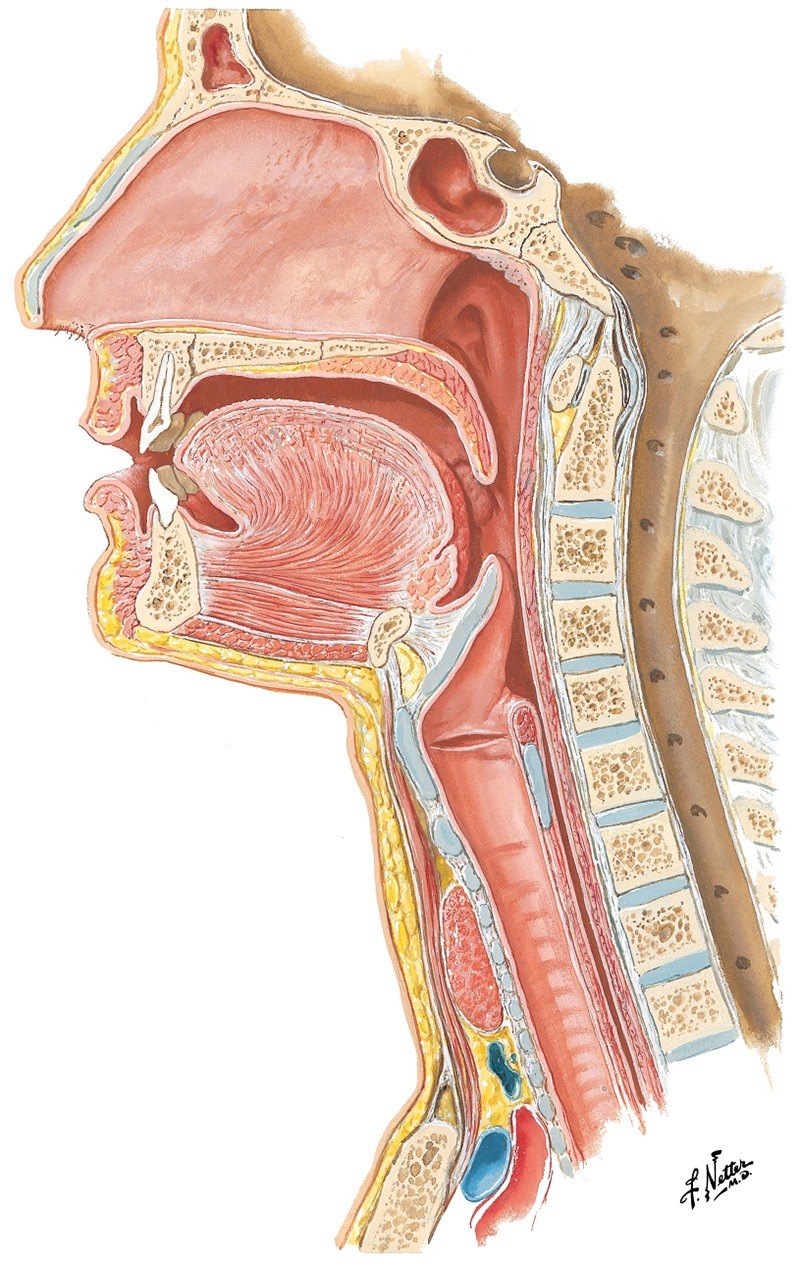
\includegraphics[width=6.4cm]{chapter2/netterVocalApparatus.jpg}};
        %\draw (0, 0) -- (8, 0);
        \draw (6.3, 5.8)--(3.4, 4.31);
        \node[align = center] at (7.5,5.8){nasal cavity};
        \draw (8.5,0)--(4.9, 0.27);
        \node[align = center] at (9.5,0){epiglottis};
        \draw (8.5,2)--(4.9, 2);
        \node[align = center] at (9.1,2){uvula};
        \draw (8.5,-2)--(4.8, -1.15);
        \node[align = center] at (9.5,-2){vocal fold};
        \draw (3.35,-2)--(5.25, -2);
        \node[align = center] at (2.6,-2){trachea};
        \draw (1, 5.8)--(2.8, 2.45);
        \node[align = center] at (0.5, 6){oral cavity};
        \draw (1.1,-1)--(3, 1.5);
        \node[align = center] at (1,-1.25){tongue};
        \draw (0.2, 0.2)--(1.8, 1.3);
        \node[align = center] at (0, 0){teeth};
        \draw (0.3, 2)--(1.2, 2.1);
        \node[align = center] at (0, 2){lip};
    \end{tikzpicture}
    \caption{Human vocal apparatus - adapted from \cite{netterAtlasHumanAnatomy2019}}
    \label{fig:vocalApparatus}
\end{figure}


\subsection{Subglottal Region}

The respiratory system, otherwise referred to as the subglottal region, comprises the lungs, diaphragm and the various airways that facilitate breathing. This system plays a crucial role with speech production by generating the airflow necessary for the vocal apparatus to produce sound. The airflow dynamics within the subglottal region are governed by both the anatomical structure of the respiratory tract and the physiological control mechanisms of breathing.

The lungs are the main part of this system, they're a pair of air-filled organs at each side of the thorax responsible for air exchange. Serving as a reservoir for air, their ability to expand and contract due to the elasticity of the lung tissue enables both the inhalation and exhalation processes. As one speaks, the controlled release of air from the lungs provides the energy source for speech, either exciting the vocal folds into vibration or just exciting the vocal tract (VT). The diaphragm, meanwhile, is a muscle located right below the lungs which contracts while inhaling, creating a vacuum that pulls air into the lungs. A similar function is also performed by the intercostal muscles which are located in between the ribs, by either expanding or contracting the rib cage \cite{zhangMechanicsHumanVoice2016}. 

\subsection{Larynx}

The larynx, often referred to as the voice box, is a crucial component of the phonatory system located in the neck atop the trachea. It is a keystone component of the apparatus, as it directs air towards the vocal folds housed within it, acting as a valve for modulating the airflow and the sound production. The larynx has a complex structure composed of connective tissues, cartilages and muscles which manipulate said cartilages, which allow for precise control over several aspects of the vocal folds such as their position, tension and length of the vocal folds. These, in turn are responsible for modulating the pitch, volume and quality of the speech.

Central to the larynx are two bands of muscle and connective tissue that stretch horizontally across the larynx, these are the vocal folds. The vocal folds are responsible for the production of voiced speech, as they vibrate when air is expelled from the lungs, creating a sound source that is then shaped by the vocal tract. The vocal folds are also responsible for the production of unvoiced speech, as they can be relaxed to allow air to pass through the larynx without any vibration. The glottis, meanwhile, is the space between the vocal folds, and it is responsible for the modulation of the airflow through the larynx.

\begin{figure}[H]
    \centering
    \begin{minipage}[H]{0.495\textwidth}
        \centering
        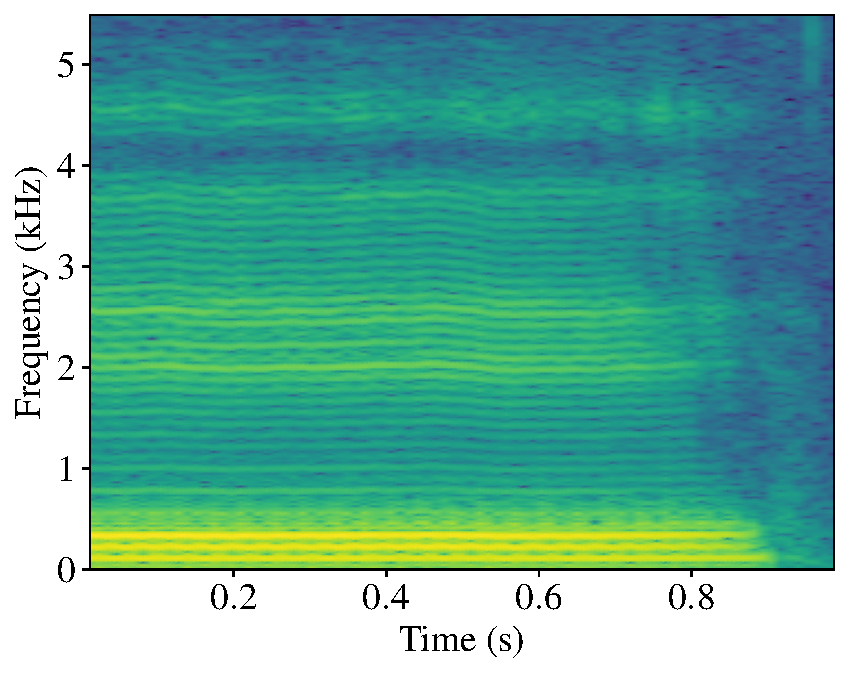
\includegraphics[width=\textwidth]{chapter2/voicedSpectrogram.pdf}
        \subcaption{}
    \end{minipage}
    \begin{minipage}[H]{0.495\textwidth}
        \centering
        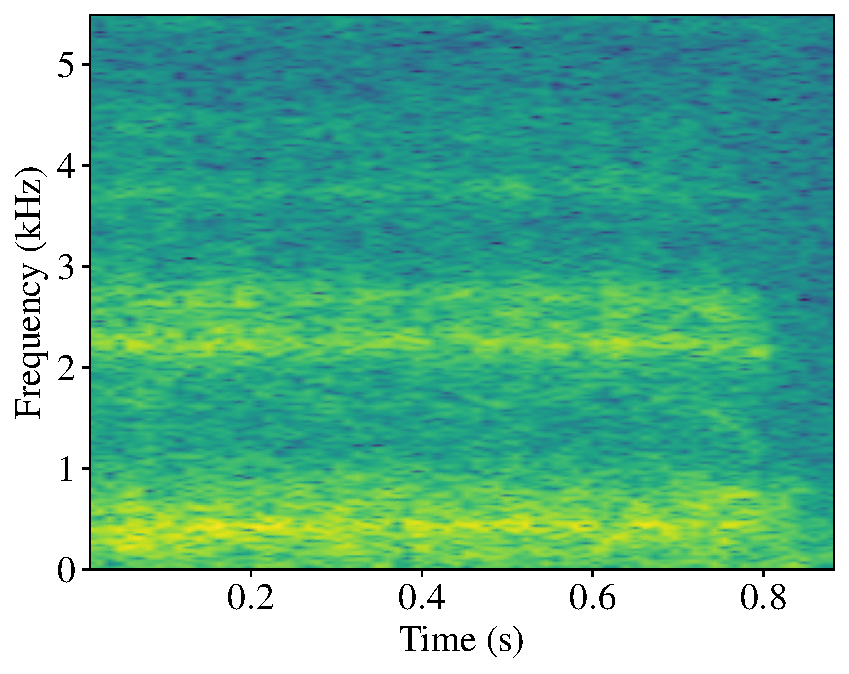
\includegraphics[width=\textwidth]{chapter2/whisperedSpectrogram.pdf}
        \subcaption{}
    \end{minipage}
    
    \caption{\centering Spectral differences between a voiced (left) and unvoiced (right) sustained vowel}
    \label{fig:voicedVsUnvoiced}
\end{figure}

Voiced speech is characterized by the presence of a fundamental frequency, which is the lowest frequency of the harmonic series produced by the vocal folds. This fundamental frequency is then responsible for the pitch of the speech signal, and it is the main difference between voiced and unvoiced speech. Unvoiced speech, on the other hand, is characterized by the lack of a fundamental frequency, as the vocal folds are relaxed and air is expelled through the open glottis. This way, the vocal tract shapes the sound spectrum in a way that the formants are still present, such that vowels are still identifiable, but without any discernable fundamental frequency, nor harmonic structure. Even so, it has been shown that whispered speech has a flatter power spectral density, this results in a noise-like sound that is then shaped by the vocal tract, as can be seen in Figure \ref{fig:voicedVsUnvoiced}.

\subsection{Supraglottal region}

The supraglottal region, encompassing the pharynx, oral cavity, and nasal cavities, forms the vocal tract, which plays a crucial role in shaping the sound produced by the vocal folds. This region acts as a resonating chamber, filtering and coloring the sound to create distinct timbre and articulation in speech. The pharynx, a muscular tube connecting the nasal and oral cavities to the larynx and esophagus, serves as a resonating cavity that amplifies and modifies sound \cite{sundbergFormantStructureArticulation2009}. The position and shape of the pharynx affects the resonant frequencies and quality of the sound produced.

Each of these structures contributes to the articulation and modulation of speech sounds. The lips alter sound by opening or closing, rounding or spreading, essential for producing various vowel and consonant sounds. The teeth provide points of contact for certain consonants, while the tongue, the most flexible articulator, shapes a wide range of speech sounds by touching or approaching different parts of the mouth. The hard palate serves as a surface for the tongue to press against, and the soft palate directs airflow through the oral or nasal cavity, crucial for producing nasal sounds \cite{mcloughlinSpeechAudioProcessing2016}.
 
The nasal cavities, air-filled spaces behind the nose, add unique resonance to the voice, especially for nasalized sounds. Airflow through the nasal cavities, controlled by the soft palate, creates nasal sounds, and the shape and size of these cavities contribute to the voice's overall resonance and quality. The supraglottal region functions as an acoustic filter, shaping the harmonic content of the sound from the vocal folds. This filtering process defines the resonant frequencies, or formants as shown later on, crucial for vowel sounds and speech intelligibility. Formants are influenced by the vocal tract's shape and length, altered by the movement of the tongue, lips, and other articulators \cite{sundbergFormantStructureArticulation2009}.


\section{Speech Modelling}

Having discussed the human vocal apparatus and its role in speech production, it is now important to discuss the models that are used to represent the speech signal, and the digital signal processing techniques that are used for speech analysis and synthesis.

\subsection{Source-Filter model}

%%
The source-filter model describes the human vocal system as a combination of sound sources and filters, relating the articulation of the speech sounds with the features of acoustic signals \cite{ferreiraComunicacoesAudiovisuaisTecnologias2009}. The original model proposed by Fant \cite{Fant1960AcousticTO} relies on the simplifying assumption that source and the filter are independent, i.e. it ignores coupling effects between these.

As per this model, there are two types of sound sources, a periodic and a non periodic one, representing the vocal folds vibration and turbulent air excitation, respectively. The filters represent the supraglottal system, namely the vocal tract, whose resonances represent the filter formants, and the radiation characteristics. A overview of this model can be seen in Figure \ref{fig:sourceFilterModel}.

\begin{figure}[H]

    \centering
    \begin{tikzpicture}
        % Outer box
        \draw (-4, -3) rectangle ++(5, 6);

        % Nodes
        \node (sum2) [draw, circle] {+};
        \node (pulse) [draw, rectangle, above left=of sum2, minimum width = 2cm, minimum height = 1cm] {Pulses};
        \node (noise) [draw, rectangle, below left=of sum2, minimum width = 2cm, minimum height = 1cm] {Noise};
        \node (vocalTract) [draw, rectangle, right= 2cm of sum2, align=center, minimum width = 2.5cm, minimum height = 1.5cm] {Vocal Tract \\ Filter $H(z)$};
        \node (lipRadiation) [draw, rectangle, right= 2cm of vocalTract, align=center, minimum width = 2.5cm, minimum height = 1.5cm] {Lip Radiation \\ Filter $L(z)$};

        % waveforms
        \node at (-0.25, 2.4) {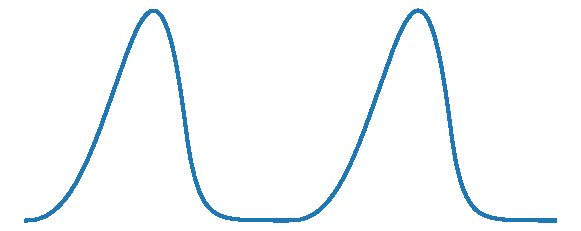
\includegraphics[width=1.5cm]{chapter2/sourceFilterDiagram/lfWave.pdf}};
        \node at (-0.25, -2.4) {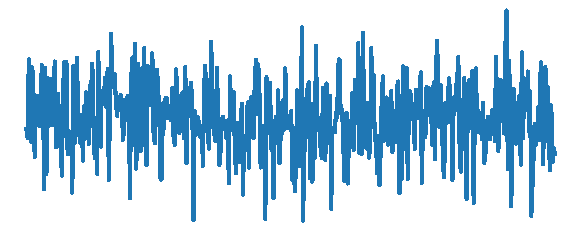
\includegraphics[width=1.5cm]{chapter2/sourceFilterDiagram/noise.pdf}};
        \node at (1.2, 0.3) {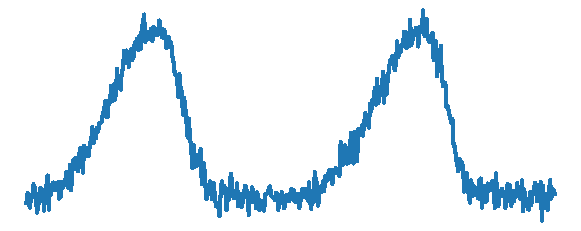
\includegraphics[width=1.5cm]{chapter2/sourceFilterDiagram/pulseNoise.pdf}};
        \node at (5.8, 0.3) {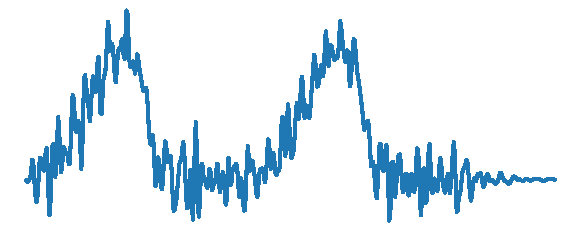
\includegraphics[width=1.5cm]{chapter2/sourceFilterDiagram/ZEROfiltered.pdf}};
        \node at (10.2, 0.3) {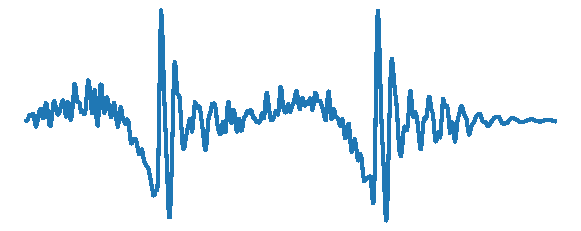
\includegraphics[width=1.5cm]{chapter2/sourceFilterDiagram/filtered.pdf}};
 
        % source/output circles
        \draw (pulse.east) ++(0.6cm, 0) circle (1mm);
        \draw (noise.east) ++(0.6cm, 0) circle (1mm);
        \draw (lipRadiation.east) ++(1.5cm, 0) circle (1mm);

        % Arrows
        \draw (pulse.east) -- ++(5mm, 0);
        \draw (noise.east) -- ++(5mm, 0);
        \draw (lipRadiation.east) -- ++(14mm, 0);
        \draw [-stealth] (sum2) -- ++(-0.6cm, 1.62cm);
        \draw [-stealth] (sum2) -- (vocalTract);
        \draw [-stealth] (vocalTract) -- (lipRadiation); 

    \end{tikzpicture}

    \caption{Source Filter Model of Voice Production}
    \label{fig:sourceFilterModel}
\end{figure}

\subsection{Glottal Flow}

Accurate and realistic estimation models of the glottal flow have been one of the most important aspects of speech synthesis and voice research. This is motivated by both the importance of the glottal flow in the speech production process and the need to understand the operational principles of the vocal folds, but also by the need to develop more efficient and realistic systems for speech synthesis or voice conversion. Here, a brief overview of some of the most important models for the glottal flow will be presented.

It is relevant to point out that the glottal flow is a measure of raw airflow through the glottis along time. However in most speech synthesis applications we are mostly concerned with the glottal flow derivative, as labial radiation can be approximated with a first order derivative filter \cite{doval:hal-00368131, Murphy2011DigitalSP}. Another important aspect of the glottal flow is that of spectral tilt, which is the difference in energy between the higher and lower frequencies of the glottal flow, which is an important aspect of voice quality and speech analysis \cite{ferreira2018on}.

%\textit{Devia explicar o spectral tilt aqui também?}


\subsubsection{Liljencrants-Fant model}

The Lijencrants-Fant (L-F) model \cite{fantFourparameterModelGlottal1985} is a five parameter mathematical model that was developed in order to represent the glottal flow during phonation, aiming to capture the physics behind the glottal flow, making it very widely used in speech synthesis and overall voice research. It is described as a piecewise mathematical function, as represented in Equation (\ref{eq:lfDerivative}), where the glottal flow derivative is described with one formula for first the opening phase, and another for the closing phase:

\begin{equation}
    g'_{LF}(t) = 
    \begin{cases}
        E_0 e^{\alpha t} \sin{\omega_g t} & , 0 \le t \le T_e \\
        - \frac{E_e}{\epsilon T_a} (e^{-\epsilon(t-T_0)} - e^{-\epsilon(T_0- T_e)}) & , T_e \le t \le T_c = T_0
    \end{cases}
    \label{eq:lfDerivative}
\end{equation}

One characteristic of the LF model is that its derivative complies with the condition that its integral across one complete period is null, this ensures that the glottal flow is volume-conserved \cite{fantFourparameterModelGlottal1985}. The glottal flow and the glottal source flow can be seen in Figure \ref{fig:lfModelGraph}. The model is defined by the parameters $E_0$ which is the maximum flow, $\alpha$ which is the damping factor, $\omega_g$ which is the angular frequency, $T_e$ which is the opening time, $E_e$ which is the end flow, $\epsilon$ which is the damping factor for the closing phase, $T_a$ which is the closing time, and $T_0$ which is the period of the glottal flow.

\begin{figure}[H]
    \centering

    \begin{minipage}[H]{0.495\textwidth}
        \centering
        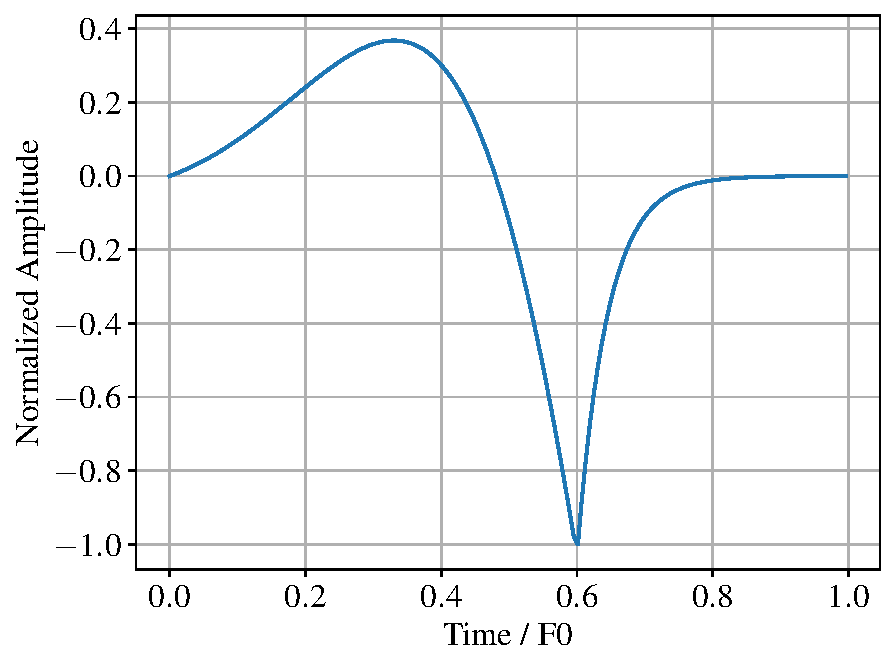
\includegraphics[width=\textwidth]{chapter2/lfFlowDerivative.pdf}
        \subcaption{}
    \end{minipage}
    \begin{minipage}[H]{0.495\textwidth}
        \centering
        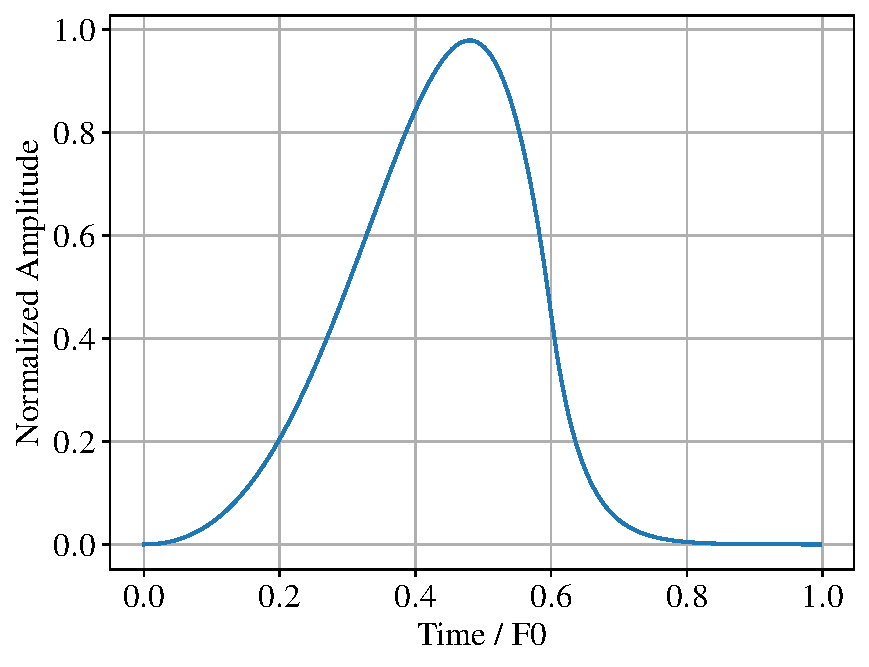
\includegraphics[width=\textwidth]{chapter2/lfFlow.pdf}
        \subcaption{}
    \end{minipage}

    \caption{\centering Lijencrants-Fant glottal flow model derivative (left) and\\corresponding glottal source flow (right)}
    \label{fig:lfModelGraph}
\end{figure}

\subsubsection{Rosenberg model}

Meanwhile, the model proposed by Rosenberg \cite{rosenbergEffectGlottalPulse1971} is a simpler model that is based on the LF model, but with a simpler mathematical representation, here shown in Equation (\ref{eq:rosenbergDerivative}). The model is composed of three parts, the first part is a sine wave that represents the opening phase, the second part is a sine wave that represents the closing phase and the third part is a null function that represents the closed phase. The glottal flow and the glottal source flow can be seen in Figure \ref{fig:rosenbergModelGraph}.

\begin{equation}
    g'_{ros}(t) = 
    \begin{cases}
        \frac{\pi A}{2T_p} \sin{\pi \frac{t}{T_p}} & 0 \le t \le T_p \\
        -\frac{\pi A}{2T_n} \sin{\frac{\pi}{2} \frac{t-T_p}{T_n}} & T_p \le t \le T_p + T_n \\
        0 & T_p + T_n \le t \le T_0
    \end{cases}
    \label{eq:rosenbergDerivative}
\end{equation}

\begin{figure}[H]
    \centering
    \begin{minipage}[H]{0.495\textwidth}
        \centering
        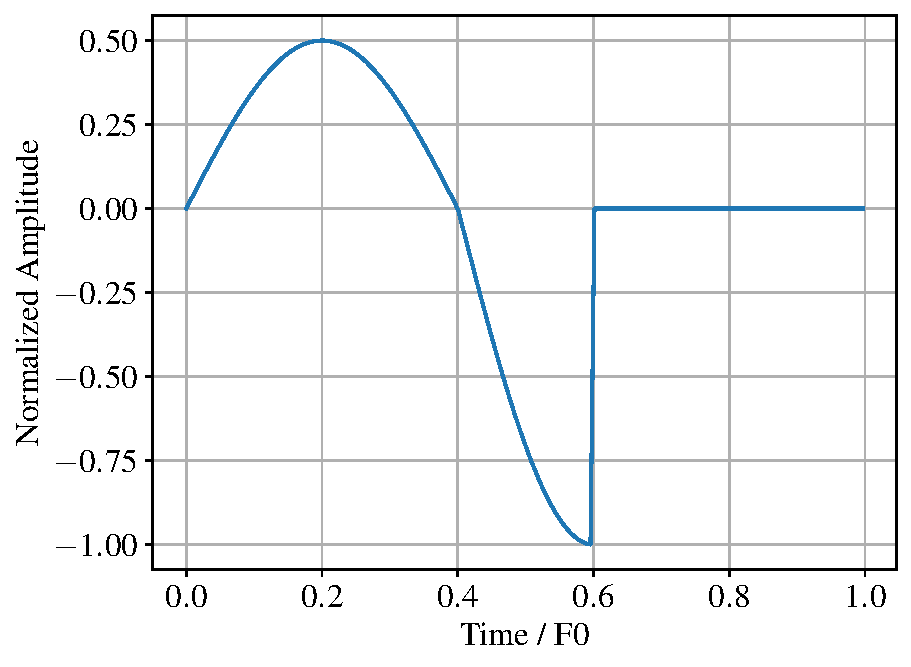
\includegraphics[width=\textwidth]{chapter2/rosenbergFlowDerivative.pdf}
        \subcaption{}
    \end{minipage}
    \begin{minipage}[H]{0.495\textwidth}
        \centering
        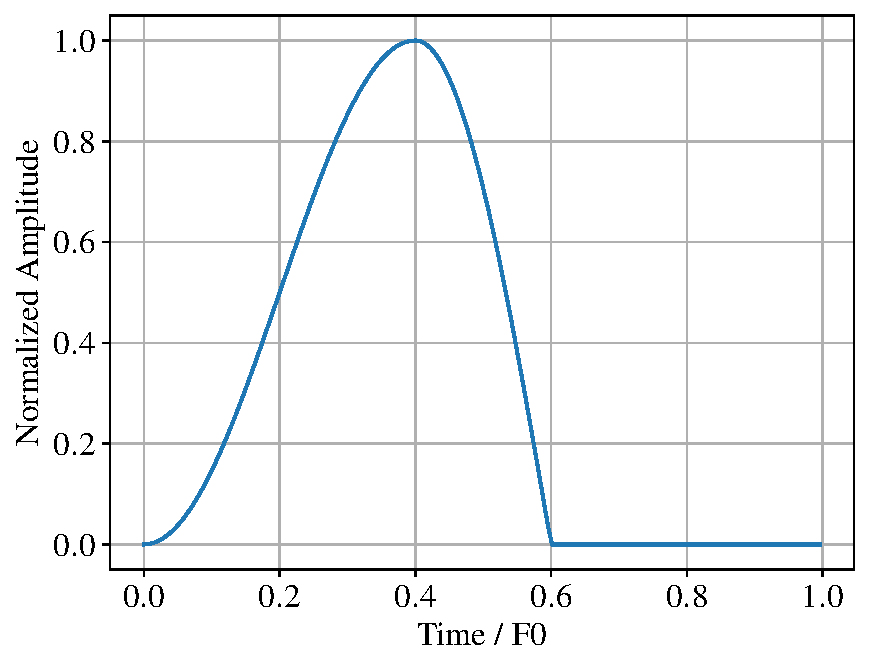
\includegraphics[width=\textwidth]{chapter2/rosenbergFlow.pdf}
        \subcaption{}
    \end{minipage}
    
    \caption{\centering Rosenberg glottal flow model derivative (left) and\\corresponding glottal source flow (right)}
    \label{fig:rosenbergModelGraph}
\end{figure}

\subsubsection{Other Glottal Flow Models}

Both the LF and Rosenberg models presented previously are just two of the many models that have been proposed to represent the glottal flow, and in this case they are both time domain models. These prove quite useful for most applications as the timing of glottal phases such as the opening time and the fundamental period are quite important for modelling the glottal flow \cite{doval:hal-00368131}. Other time domain models of the glottal flow include those proposed by Klatt and Fujisaki et. al \cite{klattAnalysisSynthesisPerception1990, 1169239}.

%Despite this, frequency-domain models are also of interest when concerning speech synthesis and processing. It has been shown that that some of the most relevant parameters for the description of voice quality are described in the frequency domain. 

\subsection{Vocal Tract Filter}

The filtering part of the source-filter model, as depicted in Figure \ref{fig:sourceFilterModel} represents the vocal tract, which is responsible for shaping the sound that is produced by the source part of the model, be it periodic glottal pulses or noisy excitation from the open glottis. This filter thus represents the joint contribution of the pharynx, the oral cavity and the nasal cavity, which are responsible for the resonances of the vocal tract, the formants \cite{doi:10.1044/jshr.3001.122}.

\subsubsection{Formants}

The different resonances and anti-resonances of the vocal tract, which result from the varying vocal tract shapes, define the frequency response of the VT filter and are known as formants. These formants are the peaks in the frequency response of the vocal tract filter, and they are responsible for the timbre of the speech signal, as they define the spectral envelope of the speech signal. 

The first three formants are generally regarded as the most contributive to the correct perception of different vowels, as they are the most prominent in the frequency response of the vocal tract filter \cite{mcloughlinSpeechAudioProcessing2016}. In fact, it is possible to synthesize direct formant frequencies in such a way as to convert a complex speech signal to just as little as 3 harmonics in what is referred to as sinewave speech \cite{Ellis2003_sws}, which can be decoded as actual speech despite sounding completely unintelligible at first. 

\begin{figure}[H]
    \centering
    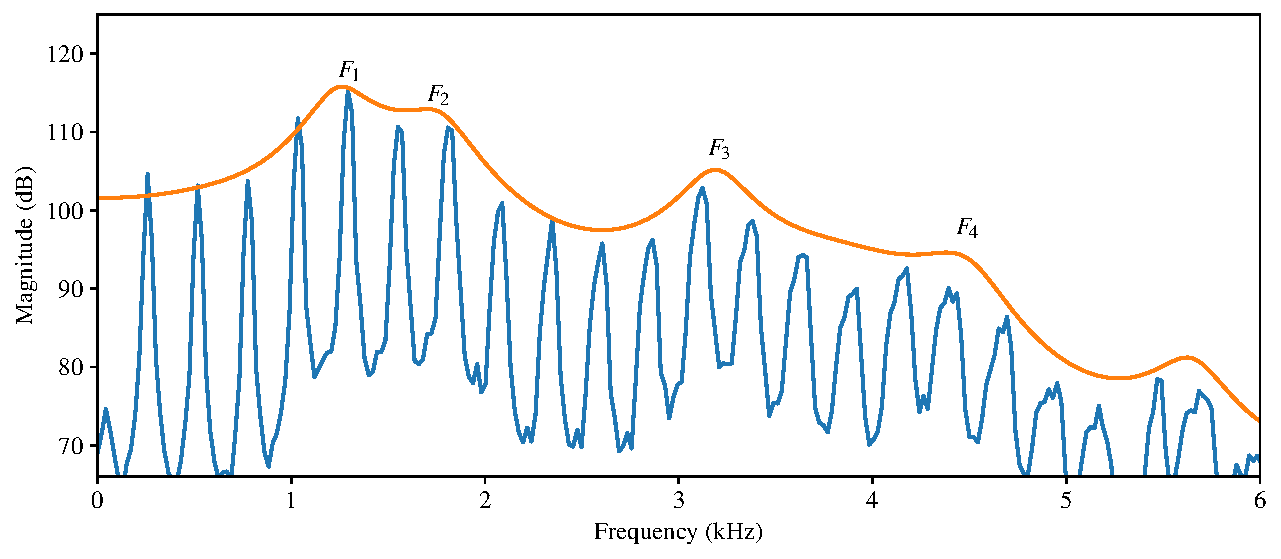
\includegraphics[width=\textwidth]{chapter2/formants.pdf}
    \caption{Formant frequencies, /a/ vowel}
    \label{fig:formants}
\end{figure}

Figure \ref{fig:formants} shows a representation of the spectral envelope (orange) for a given vowel, which was estimated from the original signal spectrum (blue) which has a clear periodic structure due to the period excitation that generated it. The formants are the peaks in the orange spectrum, and they are responsible for the timbre of the speech signal, as they define the spectral envelope of the speech signal. 

\subsubsection{Linear Predictive Coding}

Linear Predictive Coding (LPC) is possibly the most widely used method of estimating the spectral envelop, such as the one shown in Figure \ref{fig:formants}. LPC works through the assumption that an input speech signal can be approximated by a linear combination of its past samples, which is then used to estimate the filter coefficients of the vocal tract filter \cite{hayes1996statistical}. The result of LPC analysis results in a linear all-pole filter, as represented in the z-domain in Equation (\ref{eq:lpcFilter}), that best models the spectral envelope of the speech signal, which can then be used to synthesize speech signals. In fact, LPCs are most widely used in speech coding and synthesis, as they provide a good trade-off between complexity and accuracy \cite{mcloughlinSpeechAudioProcessing2016}. Often the process of estimating the filter coefficients from the spectral envelope is referred to as inverse filtering, as it is the inverse of the process of filtering the source signal with the vocal tract filter.

The process also allows for the spectral envelope of the signal to be removed, thus allowing for the residual signal to be analyzed such that the source signal can be coded into a more compact representation. This is the basis for many speech coding algorithms, such as the Mixed Excitation Linear Prediction (MELP) or Code-Excited Linear Prediction (CELP) algorithms \cite{LinearPredictionCoding2003}.

\begin{equation}
    H(z) = \frac{b_0}{1 - \sum_{i=1}^{p} a_i z^{-i}}
    \label{eq:lpcFilter}
\end{equation}

To calculate the LPC coefficients, several methods can be used but most commonly, the autocorrelation method is utilized in order to compute the $a_k$ filter denominator coefficients. As the name implies, it is based on the autocorrelation sequence $r(n)$ of the input signal $x(n)$, and can be formulated as shown in equation \ref{eq:yulewalker}. This set of equations is known as the Yule-Walker equations, and they can be solved using a least squares method, which is the most common method for estimating the LPC coefficients \cite{jackson1996digital}.

\begin{equation}
    \begin{bmatrix}
        r(0) & r(1)^* & \dots & r(N-1)^* \\
        r(1) & r(0) & \dots & \vdots \\
        \dots & \dots & \ddots & r(2)^* \\
        r(N-1) & r(N-2) & \dots & r(0) \\
    \end{bmatrix}
    \begin{bmatrix}
        a_1 \\
        a_2 \\
        \vdots \\
        a_N
    \end{bmatrix}
    =
    \begin{bmatrix}
        -r(2) \\
        -r(3) \\
        \vdots \\
        -r(N)
    \end{bmatrix}
    \label{eq:yulewalker}
\end{equation}

This being a Toeplitz system of equations, it can be solved efficiently using the Levinson-Durbin recursion \cite{hayes1996statistical}, which is an efficient algorithm that recursively estimates the filter coefficients by minimizing the prediction error. The filter coefficients are estimated by solving the Toeplitz system of equations, which is obtained from the autocorrelation function of the speech signal. In chapter \ref{chap:filt}, the implementation details of this algorithm and the computation of the autocorrelation coefficients are both discussed.

%\section{Phonetics}



\chapter{State of the Art} \label{chap:sota}

In this chapter, a brief review of the state of the art regarding whispered speech conversion  is provided, focusing on the techniques that have been previously employed to tackle the problem and their respective results and conclusions. Two main categories of whispered to normal voice conversion techniques exist: rule-based and machine learning-based approaches \cite{perrotinGlottalFlowSynthesis2020}.

\section{Rule-based}

Firstly, rule-based approaches work by modeling specific aspects of speech production in order to add voicing to the whispered signals, by defining deterministic transformation rules. These can be obtained either by empirical analysis or statistical data regarding the acoustical differences between voiced and unvoiced speech, although the simplicity of these models has an impact in both speech naturalness and quality \cite{lianWhisperNormalSpeech2019}. This can be done in several ways, as shown further in this section, but this is mostly implemented by identifying and segmenting the input whispered speech according to whether they represent potentially voiced or unvoiced segments and then adding said voicing components.

As pointed out by Perrotin et.al. \cite{perrotinGlottalFlowSynthesis2020}, these frameworks usually first decompose whisper, using linear prediction in order to estimate a parametric filter representing the spectral speech envelope, and then inverting said filter to obtain and excitation signal. Modification of the filter parameters is done afterwards, while also determining the vocalized source excitation parameters, which are then used to excite said filter and thus generate the enhanced speech.

\subsection{MELP}

One relevant work that is important to point out is that of Morris and Clement \cite{morrisReconstructionSpeechWhispers2002a}, in which a modified MELP model is employed. This is a standard way of modeling speech production, utilizing LPC to model the vocal tract, as was mentioned in Chapter \ref{chap:back}. MELP is based on mixed excitation, meaning that both periodic pulses and noise are used as excitation signals for the voiced and unvoiced/whispered sections, respectively. Both components are then mixed dynamically according to what is often referred to in literature as the aperiodicity coefficient \cite{perrotinGlottalFlowSynthesis2020}, resulting from the analysis of each signal segment, in order to produce a more natural sound. 

In \cite{morrisReconstructionSpeechWhispers2002a}, the MELP model is built upon by injecting a synthesized periodic wave to the source excitation signal, which in turn adds voicing to whispered signal, although no mention is made about the pulse shape that is used. In order to provide user feedback control, the fundamental frequency of this synthesized signal is then controlled by the sound intensity. The filter part of MELP is first modified through the implementation of a long-term, minimum phase filter, which is intended to compensate for the differences between the voiced and unvoiced signal spectrums. After the initial filtering, a correction of the formant frequencies and their bandwidth is performed, shifting them and narrowing their bands. This method does not perform any speech segmentation and instead applies permanent voicing to the low-end frequencies up to 3kHz and aperiodic excitation to the higher frequencies up to 4kHz. 

The results do show that the quality of the voice signal predicted from the whispered one is good and that the method works reasonably well, and further research \cite{huangReconstructionWhisperChinese2012} has also shown that good intelligibility can be achieved with this method. Yet, as pointed out in \cite{mcloughlinReconstructionContinuousVoiced2013,ferreiraImplantationVoicingWhispered2016}, the system is not suitable to operate in real-time applications, depending on the smoothing filter that is utilized. Furthermore, this solution does require original voice samples to be available for generating the excitation for the MELP analysis, which are not available in most practical cases.

\subsection{CELP}

Another speech codec based alternative is proposed by McLoughlin et.al. \cite{mcloughlinReconstructionPhonatedSpeech2015} using excitation codebooks with Code Excited Linear Prediction (CELP). This codec operates by first doing short-time predictions with an LPC model, thus modelling the spectral content of the speech segment, followed by an Long-term Prediction (LTP) which in turn detects the pitch. The excitations are then determined from a codebook of random Gaussian sequences using an analysis-by-synthesis approach to minimize the residual error.

This paper describes how the model is expanded upon, first by implementing formant modification and artificial glottal modulation. The formant frequencies and their amplitudes are estimated in a novel way to avoid implausible formants inferred from the noise-like nature of whisper. Preprocessing is applied to the whispered signal, firstly by identifying wether the current segment under analysis is unvoiced or not through the use of a modified G.729 detector \cite{beritelliPerformanceEvaluationComparison2002}, using both signal power and zero crossing rate to determine this. This stage is followed by a whispered phoneme classifier that analyses the spectrum for each speech segment comparing the power distribution across different bands, resulting in a classification into either plosives, fricatives or vowels. This preprocessing is then followed by a spectral enhancement stage that is applied to the whispered segments that are classified into vowels, as these are the parts where any formant imperfections do become apparent to listeners \cite{klattAnalysisSynthesisPerception1990}.



\subsection{Glottal Flow synthesis}

Perrotin et.al \cite{perrotinGlottalFlowSynthesis2020} propose a new parametric approach for converting whispered speech into natural sounding voiced speech, through the use of a sophisticated deterministic model that attempts to accurately parameterize both the glottal pulse excitation and the vocal tract. This is slightly different in function from the previously presented solutions as the authors claim that this approach is voice-based, meaning that the source model does not consider only the excitation but also the glottis filter and the lip radiation. This is opposed to the previous methods which would fall into the DSP-based category of modelling, where the source is just the excitation while the filtering is a result of the glottis, VT and the lips.

The proposed method synthesizes an excitation source based on a pulse train combination of harmonic frequencies, whose frequencies are based on a fundamental frequency multiplied by a random factor above a certain $F_{VUV}$ frequency. The phase is also slightly randomized for each harmonic as to introduce natural sounding roughness. This is done after the whispered signal goes through a preprocessing stage, where inverse filtering is done to first obtain both vocal tract and glottis filter coefficients, in this case using GFM-IAIF \cite{alkuGlottalWaveAnalysis1992} to estimate both from the whispered signal. A new glottis filter is then synthesized based on configurable parameters which allow the user to indicate the range of effort and tension \cite{feugereCantorDigitalisChironomic2017} for the synthesized signal. The synthesized excitation is then filtered through the newly synthesized filter and mixed with the original glottal flow derivative according to whether the current segment is voiced or unvoiced. Finally, the original VT filter filters these segments. Another important aspect that is introduced in this work is the use of the spectral centre of gravity in order to determine the voiced/unvoiced decision, which is then used to determine the amount of voicing and noise that is added to the signal, an idea that also inspires our work, as detailed in Chapter \ref{chap:overlapAdd}.

The authors then go on to evaluate this method through subjective and objective tests to measure the naturalness of synthesized speech and the accuracy of voiced/unvoiced (V/UV) decisions, using a MUSHRA \cite{internationaltelecommunicationunionBS15343Method2015} perceptual testing environment. The subjective experiment involved comparing the proposed glottal source model against the baseline pulse train method and natural speech sources using the wTIMIT database, which contains pairs of phonetically balanced sentences. The new glottal source significantly outperformed the baseline pulse train method in terms of naturalness, receiving higher median scores. The accuracy of V/UV decisions revealed a total V/UV error rate of 17.7\%, with a significant negative correlation between the UV-to-V error rate and naturalness scores. Sentences with fewer unvoiced consonants received higher scores, indicating sensitivity to V/UV decisions.


\subsection{Other Speech Conversion Approaches}

Toda et. al. \cite{todaStatisticalVoiceConversion2012} explore advanced methods to enhance body-conducted unvoiced speech for silent speech communication using a nonaudible murmur (NAM) microphone. This type of microphone captures very soft unvoiced speech, such as NAM or whispered voices, while keeping emitted sounds almost inaudible to those around the speaker. The main challenge addressed in the article is the unnatural and less intelligible quality of body-conducted unvoiced speech due to acoustic changes caused by body conduction.

To tackle this issue, the authors propose two primary voice conversion methods. The first method, NAM-to-Speech, aims to convert NAM to normal speech to improve intelligibility. However, this method often results in degraded naturalness because it is challenging to estimate natural fundamental frequency contours from unvoiced speech. The second method, NAM-to-Whisper, converts NAM to a whispered voice, which is a familiar form of unvoiced speech and thus easier to convert accurately. This method significantly enhances both the intelligibility and naturalness of the converted speech compared to NAM-to-Speech. The conversion process relies on Gaussian mixture models (GMMs) to probabilistically transform the acoustic features of body-conducted unvoiced speech into those of natural voices.

Experimental evaluations demonstrate the effectiveness of these proposed methods. NAM-to-Whisper outperforms NAM-to-Speech in both intelligibility and naturalness, making it a more promising solution for enhancing body-conducted unvoiced speech. Additionally, the methods are extended to handle both NAM and body-conducted whispered voice (BCW), improving the versatility and robustness of the system. The article underscores the potential of these statistical voice conversion techniques to overcome the inherent problems of silent speech communication, paving the way for more universal and private speech communication methods.

%Non-audible nurmurs\dots
%
%Statistical Voice Conversion Techniques for Body-Conducted Unvoiced Speech Enhancement \cite{todaStatisticalVoiceConversion2012}
%
%Some have also studied using ingressive speech in order to \dots

\section{Machine Learning Approaches}

As opposed to rule-based, ML approaches rely on learning algorithms to reconstruct voiced speech from whispers. These algorithms are trained on matched data points of natural and whispered speech, requiring a specially curated dataset although some approaches avoid this necessity through non-parallel training models. Recent advancements have introduced a variety of machine learning frameworks to tackle the challenges imposed by WSC, namely the intricate task of estimating the fundamental frequency $F_0$ contour \cite{oliveiraMachineLearningApproaches2022}, and the automated segmentation of speech, both crucial for the prosody characteristics of natural speech. 

Examples of ML approaches in this field are mostly based on Deep Neural Network (DNN) architectures, including Generative Adversarial Networks, Autoencoder, Bidirectional Long Short-Term Memory and Transformer frameworks. One main issue of most of the papers analyzed in \cite{oliveiraMachineLearningApproaches2022} is that most apporaches did not do any sort of perceptual testing and opt to utilize other objective metrics to evaluate the performance of their systems, such as utilizing speech recognition technologies for this purpose. In the following sections, a non-exhaustive review of the most relevant works in this field is presented. It is important to note that the field of WSC can be seen as a niche within a niche in research, as the amount of deep learning audio research, although growing, is still relatively small when compared to other fields such as image processing or natural language processing.

\subsection{Long Short-Term Memory}

In \cite{lianWhisperNormalSpeech2019}, a sequence-to-sequence model is proposed for whispered speech conversion. The Seq2Seq model used is based on a LSTM architecture \cite{cho2014learningphraserepresentationsusing}, which was a pioneering architecture that has been utilized successfully in many natural language processing applications. This proposed model is trained on a dataset of whispered and normal speech pairs, and is capable of generating natural sounding speech from whispered input. The model is composed of two main components, an encoder and a decoder, which are both based on Long Short-Term Memory (LSTM) networks. The encoder is responsible for encoding the input whispered speech, while the decoder generates the normal speech from the encoded representation. The model is trained using a combination of the mean squared error loss and the mel-cepstral distortion loss, which is a measure of the difference between the mel-cepstral coefficients of the generated and target speech.

Experimental results validate the effectiveness of the proposed method which exhibits superior performance across different metrics, such as Mel Cepstral Distance (CD) and Short-Time objective Intelligibility (STOI) when compared to other state-of-the-art methods. The authors also conducted a subjective evaluation of the generated speech, which showed that the proposed method outperformed other methods such as Gaussian Mixture Models (GMM) and Bidirectional LSTMs \cite{todaNAMtospeechConversionGaussian2005, meenakshiWhisperedSpeechNeutral2018} in terms of naturalness and intelligibility.

\subsection{Generative Adversarial Networks}

Parmar et.al. \cite{parmarEffectivenessCrossdomainArchitectures2019} investigated the application of Generative Adversarial Networks (GANs) to model the intricate differences between whispered and normal speech. Two main architectures are focused on, the first being a CycleGAN \cite{zhu2020unpairedimagetoimagetranslationusing} based model and the second being a modified DiscoGAN \cite{shahNovelMMSEDiscoGAN2018}, which are both trained on a dataset of whispered and normal speech pairs. Both models aim to learn the cross-domain relationships, i.e. the mapping between whispered and normal speech enhancing the quality and naturalness.

The authors conducted comprehensive experiments using the whispered TIMIT (wTIMIT) database, training and evaluating their models on parallel datasets of whispered and normal speech. Objective measures such as Mel Cepstral Distortion (MCD) and Root Mean Square Error (RMSE) of log(F0) were used to assess the performance of the conversion systems. The results demonstrated that both DiscoGAN and CycleGAN significantly outperformed traditional GAN models in reducing MCD and RMSE. Interestingly, while DiscoGAN yielded better objective results, CycleGAN was preferred in subjective evaluations for its naturalness, where this preference is attributed to the differences in their loss functions. Findings indicate that these models can produce more natural-sounding normal speech from whispered input, with CycleGAN being particularly favored for its subjective performance. The authors suggest that further improvements can be achieved by exploring high-quality vocoders such as WaveNet \cite{oord2017parallelwavenetfasthighfidelity} to enhance the voice quality of the converted speech.

Another GAN based architecture as been deployed by Patel et. al. \cite{patelCinCGANEffectiveF02021} to improve the conversion of whispered speech to normal speech by predicting the fundamental frequency (F0). The authors introduce the Cycle-in-Cycle GAN (CinC-GAN), an advanced version of CycleGAN, designed to enhance the accuracy of F0 prediction without compromising the mapping of Mel Cepstral Coefficients (MCC). This is crucial because traditional CycleGAN methods, which rely on separate models for MCC mapping and F0 prediction, often introduce significant non-linear noise in the predicted F0 due to the non-linear DNN layers at the network's output.

This CinC-GAN architecture introduces a joint training methodology that concurrently trains for MCC mapping and F0 prediction. This holistic approach has been shown to reduce the non-linear noise that typically affects the output of sequentially trained models. Finally the paper reports that CinC-GAN significantly outperforms the baseline CycleGAN in both objective and subjective evaluations. Objective metrics, such as Mel Cepstral Distortion (MCD) and Root Mean Square Error (RMSE) of log(F0) also show substantial improvements. Additionally, subjective evaluations reveal that CinC-GAN delivers superior naturalness scores across both seen and unseen speakers, underscoring its effectiveness in generating more natural-sounding speech.z 

\subsection{Transformer Networks}

Transformer networks have more recently been widely used for many natural language processing applications, as their attention mechanisms allow for more efficient handling of sequential data, such as text information or audio signals, on sequence-to-sequence tasks when compared to traditional RNNs (Recurrent Neural Networks) and CNNs (Convolutional Neural Networks). First introduced in the paper by \cite{vaswani2023attention}, the key components of the transformer are it's attention mechanism, which allow the networks to weigh different input tokens in a sequence when encoding each token, and the positional encoding, which allows the network to understand the order of the tokens in the sequence.

Nirajan et al. \cite{niranjanEndtoEndWhisperNatural2021} propose an {\it end-to-end} approach to WSC by adapting a conventional transformer network. This method incorporates three key components, first the standard encoder and decoder found in transformer architectures, along with an additional encoder designed to predict triphones, which are sequences of three phonemes. Their implementation involves two distinct networks; one processes Mel-frequency Cepstral Coefficients (MFCCs), and the other processes smooth spectral features. Although no perceptual tests were conducted, the findings indicate a generally lower word error rate in automatic speech recognition (ASR) systems when using the MFCC-based network.

On the other hand, more recent work conducted by Rekimoto \cite{rekimotoWESPERZeroshotRealtime2023} takes advantage of transformer networks in order to perform speech conversion in what is claimed to be real-time. The system architecture proposed consists on a Speech-to-Unit encoder network that trained on both whispered and normal speech, and it is essentially a modified version of BERT that learns to map both types of data samples to common speech units in a self-supervised manner. Then a separate decoder network based on a simplified version of Microsoft's Fastspeech II \cite{ren2022fastspeech2fasthighquality} handles the conversion of the individual units to mel-spectrograms, which are then converted back to audio using Hifi-GAN \cite{kong2020hifigangenerativeadversarialnetworks}. 

The results of the WESPER system, as detailed in the study, indicate a significant improvement in the perceptual quality of whispered speech when converted to normal speech. Evaluations using Mean Opinion Score (MOS) and MUSHRA \cite{internationaltelecommunicationunionBS15343Method2015} methodologies demonstrated that the converted voices scored higher than whispered voices in terms of quality, naturalness, and prosody preservation. Specifically, the converted speech showed statistically significant improvements in perceived naturalness and reduced hoarseness. Additionally, for individuals with Vocal Fold Polyps (VFP), Spasmodic Dysphonia (SD), and hearing impairments, the converted speech exhibited enhanced intelligibility and naturalness. The study concludes that WESPER offers an arguably real-time solution for effectively converting whispered speech, without compromising on the natural prosody of the original speech.



%\section{Research at FEUP}



\chapter{Glottal Pulse Generation}
\label{chap:pulseGen}

In this section the synthesis mechanism of the glottal pulse is described, as it serves as the basis for the type of speech reconstruction framework that is built upon in the following sections. As mentioned in chapter \ref{chap:back}, the glottal pulse is the voiced excitation signal for the vocal tract model, which gets mixed with noise in order to replicate actual voicing. %The glottal pulse is generated by the glottal source model, which is a simplified model of the human vocal folds. 

The main goal of the proposed solution is to perform the filtering of the source glottal waveform on a pulse-by-pulse basis, in order to achieve a more natural sounding synthetic voice signal, without any hard filter changes that occur in some LPC codecs. The mechanism behind this is explained in further sections, as in this one we are just concerned with the modelling of each individual pulse waveform.

\section{Processing and development platform}

Besides this main last topic, this chapter also goes through the implementation of the glottal pulse generation in real-time, utilizing an STM32 based board. Also, a Python based environment was used in order to validate the functionality and the performance of the algorithms as a baseline to the real-time implementation using the STM32 platform. During previous work on the DyNaVoiceR project \cite{goncalvesVozeamentoSinteticoVoz2023}, the STM32-F746G discovery kit \cite{stmicroelectronicsSTM32F746NGDiscoveryKit} has also been utilized in order to preform real-time voice conversion, as it includes not only several key hardware features that facilitate audio processing such as the Direct Memory Access (DMA) controller and the built-in audio codec, but also a wide range of libraries meant for signal processing applications. As such, this development board was chosen as the platform for the real-time implementation of the voice conversion system.

One important requirement for real-time audio processing is that of latency, as it has been shown that humans are quite sensitive to the delay between audio signals. This is called the precedence effect, where it has been shown that short delays from 5 to 30 ms are perceived as a single sound source \cite{Litovsky1999ThePE}. It is also the reason why we can perceive the direction of a sound source even when the sound reaches one ear ever so slightly before the other. Another important aspect is that of the delay between the audio signal and the visual signal, which is known as the lip-sync effect, and is also quite noticeable when the delay between the two is greater than 100 ms \dots

\subsection{Python Development Environment}

The Python environment used for the development of the pulse generation algorithm was mainly based on the NumPy \cite{2020NumPy-Array} library for numerical computation, and SciPy \cite{2020SciPy-NMeth} for most signal processing functions. The main advantage of using Python for this task is that it is a high-level language and allowed for rapid prototyping of the algorithms, and it has a wide range of libraries that can be used for signal processing applications. The main disadvantage of using Python for this task is that its interpreter is quite slow, and it is not suitable for unoptimized real-time audio processing applications such as the ones that were run during prototyping. PyAudio has also been considered for real-time audio processing, as it is essentially a wrapper for PortAudio. This ended up not working, as the processing delay as been found to be too high even for the simple applications. Other libraries that were utilized included Matplotlib for plotting the results and librosa for some audio processing functions such as resample and fundamental pitch tracking.

\subsection{STM32 Development Environment}

For the development of the realtime implementation of the system the Arm Keil MDK uVision IDE was utilized as the sole development environment, as it includes all the tooling needed for writing, compiling and flashing code to the STM32 board. Also several libraries are available which include ready made methods for the STM32 board such as Fast Fourier Transforms and complex number arithmetic. Furthermore, extensive code examples for the Discovery kits are available, which were used as a starting point for using the DMA controller and the audio codec. Figure \ref{fig:stm32testEnv} shows the development and testing environment for the STM32 board along with the audio interface that was used as both input and output for the system.

\begin{figure}[H]
    \centering
    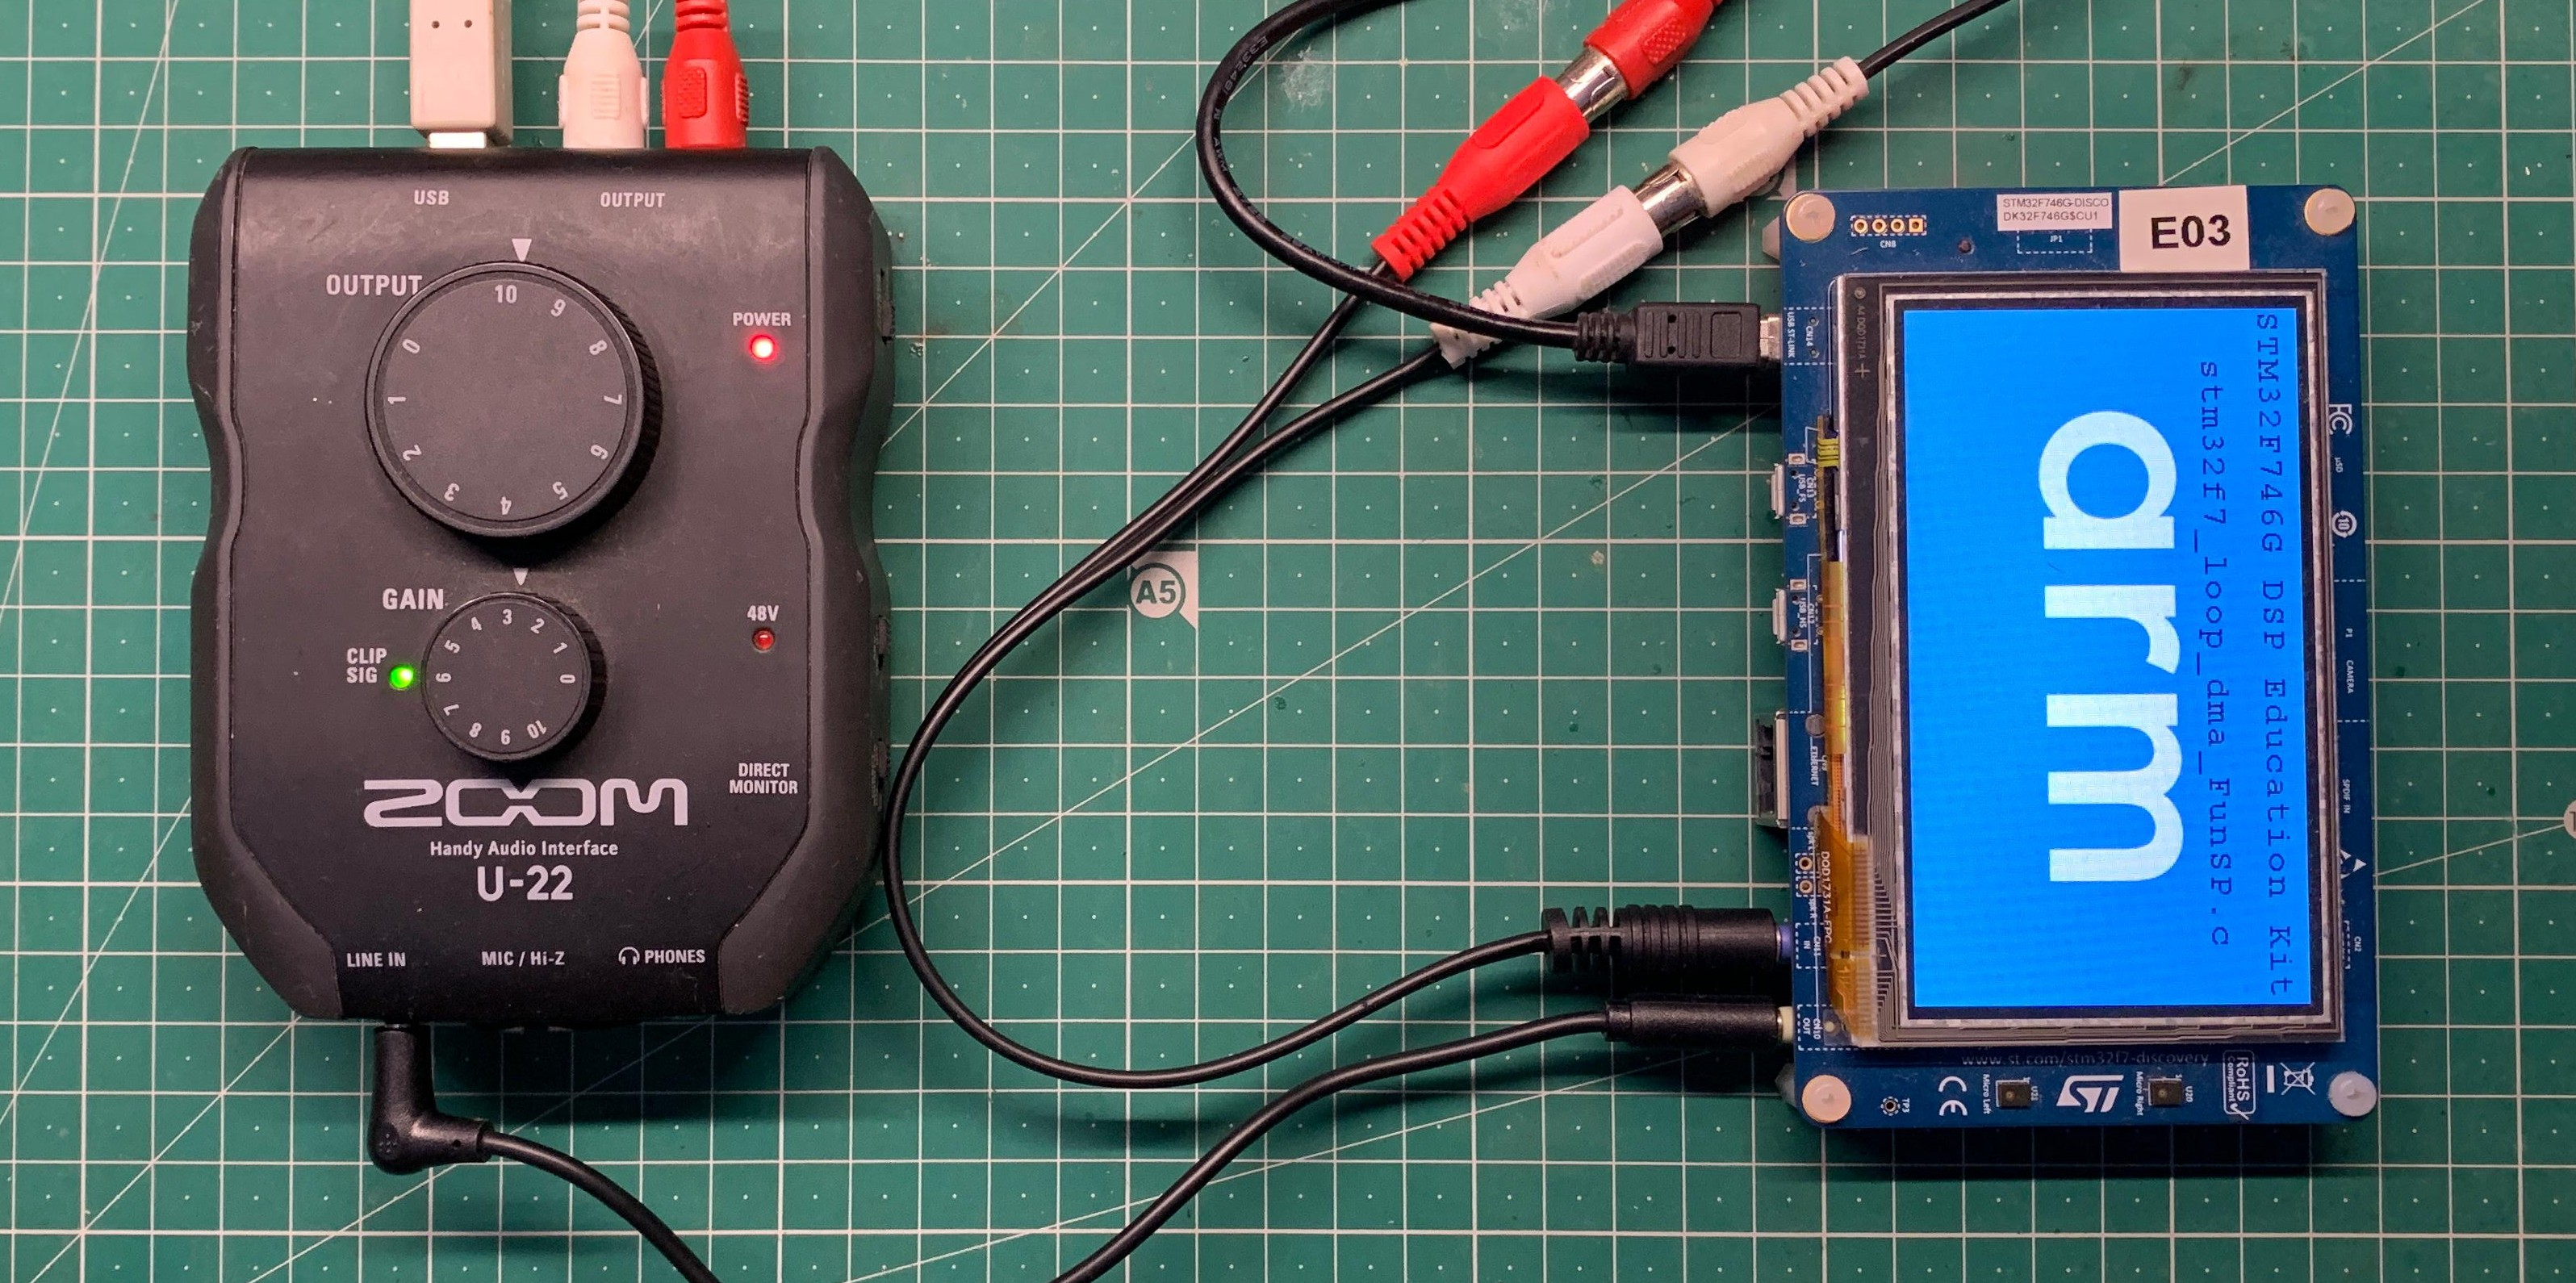
\includegraphics[width = 0.7\textwidth]{chapter4/testing.jpeg}
    \caption{STM32 development and testing environment}
    \label{fig:stm32testEnv}
\end{figure}


In \cite{goncalvesVozeamentoSinteticoVoz2023} it was then determined that the STM32 should be setup to operate at a sampling frequency of 22050Hz and utilizing DMA input and output buffers of 512 samples each. This had been measured to result in a minimum DMA processing latency of about $47.9$ ms.

\section{Pulse Template Generation}

As was discussed in chapter \ref{chap:back}, the glottal pulse (and for that matter, the glottal pulse derivate) are the basis of voiced speech, and a good implementation of this is key to having natural sounding synthetic speech. The LF-model \cite{fantFourparameterModelGlottal1985} is a obvious choice for this, and can be modelled by Equations (\ref{eq:lfDerivative}). For the purposes of this work, the implementation that is provided in the VOICEBOX Matlab library \cite{brooksVOICEBOXSpeechProcessing2018}, has been adapted to work in Python using NumPy in \texttt{v\_glotlf()}, as is shown in Listing \ref{lst:lfPulse}.

% secalhar passo isto para o anexo não? 
\begin{lstlisting}[language=Python, caption={LF glottal flow derivate method - \texttt{v\_glotlf()}}, label={lst:lfPulse}, style=mystyle]
def v_glotlf(t):
    p = np.array([0.6, 0.1, 0.2]) # [T_e, E_0/E_e, 1 - t_p/t_e]

    tt = t - np.floor(t)  # only interested in the fractional part of t

    te = p[0]
    mtc = te - 1
    e0 = 1
    wa = np.pi / (te * (1 - p[2]))
    a = -np.log(-p[1] * np.sin(wa * te)) / te
    inta = e0 * ((wa / np.tan(wa * te) - a) / p[1] + wa) / (a**2 + wa**2)

    rb0 = p[1] * inta
    rb = rb0
    for _ in range(4):
        kk = 1 - np.exp(mtc / rb)
        err = rb + mtc * (1 / kk - 1) - rb0
        derr = 1 - (1 - kk) * (mtc / rb / kk)**2
        rb = rb - err / derr

    e1 = 1 / (p[1] * (1 - np.exp(mtc / rb)))
    ta = tt < te
    tb = ~ta

    u = np.zeros_like(tt)
    u[ta] = e0 * np.exp(a * tt[ta]) * np.sin(wa * tt[ta])
    u[tb] = e1 * (np.exp(mtc / rb) - np.exp((te - tt[tb]) / rb))

    return u
\end{lstlisting}

This code defines the default LF-model parameters \cite{brooksVOICEBOXSpeechProcessing2018} as the following: $E_0 = 0.1$, $E_e = 1.0$, $T_e = 0.6T_0$ and $T_e = 0.48T_0$, which provide a good baseline from which we can model the glottal pulse from. These prove to be sufficiently accurate for the intended application as we will demonstrate on during the perceptual testing. In Figure \ref{fig:lfGFD} the resulting pulse waveform is shown, indicating the two time points that define the LF curve, and from which all other parameters are computed from.

\begin{figure}[H]
    \centering
    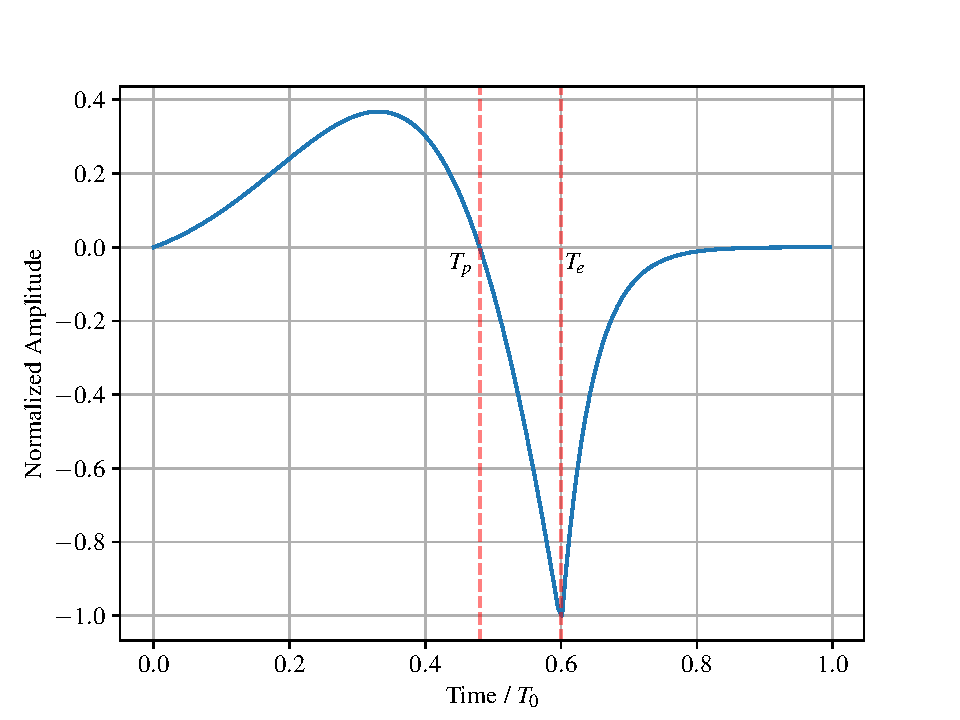
\includegraphics[width = 0.8\textwidth]{chapter4/lfDerivative.pdf}
    \caption{LF Glottal Flow Derivative model}
    \label{fig:lfGFD}
\end{figure}

\subsection{Harmonic Analysis}

Since we have to generate the glottal pulse in real-time, we need to have a way to generate the pulse waveform in a computationally efficient manner. One way to do this is to expand the waveform into its Fourier series \cite{hsu2010schaum}, and summing the resulting harmonic frequencies as shown in Equation (\ref{eq:lfFourier}), where $\text{Mag}_i$ and $\phi_i$ represent the magnitude and the phase of the i-th harmonic respectively.

\begin{equation}
    \hat{g}_{LF}(t) = \sum_{i=0}^{N_{harm}} \text{Mag}_i \sin \left (2\pi F_0 t + \phi_i \right )
    \label{eq:lfFourier}
\end{equation}

The magnitude and phase of each harmonic can be computed using Equations (\ref{eq:fourierSeries}), where $a_i$ and $b_i$ are the coefficients of the Fourier series, and $\text{Mag}_i$ and $\phi_i$ are the magnitude and phase of the i-th harmonic respectively. 

\begin{equation}
    \begin{cases}
        a_i = 2 F_0 \sum_{i=1}^{N_{harm}} LF(t) \cos \left (2\pi i F_0 t \right ) \\
        b_i = 2 F_0 \sum_{i=1}^{N_{harm}} LF(t) \sin \left (2\pi i F_0 t \right ) \\
        \text{Mag}_i = \sqrt{a_i^2 + b_i^2}\\
        \phi_i = \arctan{\left (\frac{b_i}{a_i} \right )}
    \end{cases}
    \label{eq:fourierSeries}
\end{equation}

One important aspect is that enough harmonics are generated in order to fill the entire frequency spectrum, such that when they are filtered by the vocal tract model, the entire spectrum is coloured. As such, the number of necessary harmonics can be determined by

\begin{equation}
    N_{harm} = \frac{F_s}{2F_0} \text{,}
    \label{eq:harmonics}
\end{equation}

\noindent where $F_s$ is the sampling frequency of the signal, and $F_0$ is the fundamental frequency of the signal. Assuming the worst possible case of $F_0 = 60Hz$, in the case of a very low pitched voice, then $N_{harm} \ge 186$. This is a good rule of thumb for determining the number of harmonics that need to be generated in order to have a good representation of the pulse waveform, that is coloured through the entire Nyquist band.

Another way to represent the phase is using each harmonics' Normalized Relative Delay (NRD) coefficients \cite{ferreira2018holistic}, which are defined as the phase of each harmonic relative to that of the fundamental frequency. It has been shown that the glottal pulse NRDs are fairly linear as the harmonic number increases, which simplifies the code. Thus we can just compute the first 20 harmonics and then extrapolate the rest. The NRD coefficients for a periodic wave can be determined by the following equation:

\begin{equation}
    \text{NRD}_i = \frac{\phi_i- i\phi_0}{2\pi} \text{.}
    \label{eq:nrd}
\end{equation}

From this, the pulse generation can be done in real-time, by computing the magnitude and NRD of each harmonic \cite{ferreiraImpactShiftInvariantHarmonic2020}, and then summing them for the duration of a single period $T$ in order to generate the pulse waveform, as is shown in Equation (\ref{eq:nrdLfgfd}). This is done in the following subsection.

\begin{equation}
    g'_f(t) = \sum_{l=1}^L \frac{\text{Mag}_l}{l} \sin \left (\frac{2\pi}{T}lt + \text{NRD}_l \right )
    \label{eq:nrdLfgfd}
\end{equation}

\subsection{Real-time Pulse Generation}

As the STM32 board is being setup to operate using DMA processing, the pulse generation is done in real-time, as opposed to pre-generating the pulses and storing them in memory. This is done by utilizing the DMA controller to continuously process the audio buffer, and generate the glottal pulse on the fly. The flowchart for the pulse generation is shown in Figure \ref{fig:pulseGenFlow}, and the code for the pulse generation in C is shown in listing \ref{lst:genPulse}.

\begin{lstlisting}[language=C, caption={Pulse generation function.}, label={lst:genPulse}]
uint16_t genPulse(float32_t fs, float32_t f0, float32_t * pulseBuff, float32_t gain){
    float32_t T0 = 1/f0;
    float32_t Ts = 1/fs;

    uint16_t outLen = getPulseLen(fs, f0); // compute the output length
    float32_t max = 0;

    // zero out the pulse buffer before writing to it
    memset(pulseBuff, 0.0f, MAX_PULSE_BUFFER);

    float32_t magn, phase, argsin;
    for (int32_t i = 0; i < Lharm; i++){ // Compute and accumulate each harmonic
        magn = mag[i]; 
        phase = 2 * PI * nrd[i];
        argsin = (i+1) * 2 * PI * f0 * Ts;

        for (int j = 0; j < outLen; j++) // generate entire waveform
            pulseBuff[j] += magn * sin(argsin * j + phase); 
    }
    
    // Determine max sample for normalization
    float32_t sample;
    for (int32_t i = 0; i < outLen; i++){
        sample = (float32_t) fabs((double) pulseBuff[i]);
        
        if(sample > max) max = sample; 
    }
    
    // normalize
    float32_t scale = gain * (INT16_MAX) / max;
    for (int32_t i = 0; i < outLen; i++)
        pulseBuff[i] = scale * pulseBuff[i];
    
    return outLen;
}
\end{lstlisting}

The DMA processing in this case works by means of a double buffering method, where the DMA controller is set to transfer both the input and output to one of two buffer sets, either PING or PONG, while the CPU is free to do processing on the data from the other set. In this case, the mechanism is set on the \texttt{process\_buffer()} function, as can be seen in listing \ref{lst:processBuffer}, where the input is copied directly to the right input channel for validation, while the output is set from the first half of the \texttt{mainBuff} vector.

In this case, \texttt{mainBuff} is the buffer that is used to store the pulse waveform that is twice as long as the output audio buffer (i.e. 1024 samples long). This is done in order to allow the pulse generation to overlap between the two halves of the buffer, and to allow the pulse generation to be continuous across subsequent frames. 

\begin{figure}[H]
    \centering
    \resizebox{0.4\textwidth}{!}{
    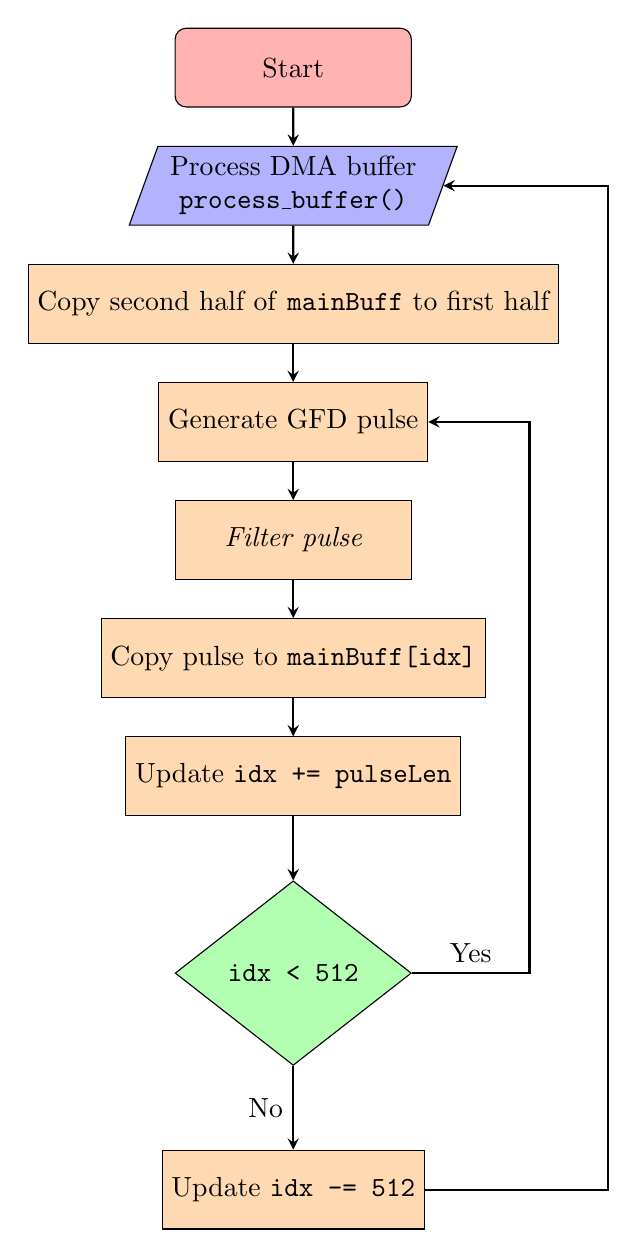
\begin{tikzpicture}[auto, node distance=1.5cm, >=latex']
        \node (start) [startstop] {Start};
        \node (in1) [io, below of=start, align=center] {Process DMA buffer \\ \texttt{process\_buffer()}};
        \node (copy) [process, below of=in1] {Copy second half of \texttt{mainBuff} to first half};
        \node (pulseGen) [process, below of=copy] {Generate GFD pulse};
        \node (pulseFilt) [process, below of=pulseGen] {\it Filter pulse};
        \node (pulsePlacement) [process, below of=pulseFilt] {Copy pulse to \texttt{mainBuff[idx]}};
        \node (indexUpdate) [process, below of=pulsePlacement] {Update \texttt{idx += pulseLen}};
        \node (pulseEnd) [decision, below of=indexUpdate, yshift=-1cm] {\texttt{idx < 512}}; % < 512 samples
        \node (indexDecrement) [process, below of=pulseEnd, yshift=-1.25cm] {Update \texttt{idx -= 512}};

        \draw [arrow] (start) -- (in1);
        \draw [arrow] (in1) -- (copy);
        \draw [arrow] (copy) -- (pulseGen);
        \draw [arrow] (pulseGen) -- (pulseFilt);
        \draw [arrow] (pulseFilt) -- (pulsePlacement);
        \draw [arrow] (pulsePlacement) -- (indexUpdate);
        \draw [arrow] (indexUpdate) -- (pulseEnd);
        \draw [arrow] (pulseEnd) -- node[anchor=east] {No} (indexDecrement);
        \draw [arrow] (pulseEnd) -- node[anchor=south] {Yes} ++(3,0) |- (pulseGen);
        \draw [arrow] (indexDecrement) -- ++(4, 0) |- (in1);
    \end{tikzpicture}
    }
    \caption{Flowchart of the pulse generation algorithm.}
    \label{fig:pulseGenFlow}
\end{figure}

The pulse generation function is then called in order to generate the glottal pulse waveform, which is then copied to the main buffer, and then the index is updated in order to generate the next pulse. This process is repeated until the entire buffer is processed, and then the DMA controller is set to transfer the main buffer back to the audio buffer, and the audio signal is then output to the audio codec. The code responsible for this can be found in listing \ref{lst:mainPulseGen}.


It is worth noting that the pulse generation algorithm that is shown in Figure \ref{fig:pulseGenFlow} includes the filtering operation after the pulse generation, which was not present in this case as it was unimplemented at the time.

\subsubsection{Real-time Pulse Generation Results} 

In order to validate not only the realtime pulse generation algorithm, but all the other algorithms on the STM32 platform, the setup from Figure \ref{fig:stm32testEnv} was utilized. This testing environment consisted of the following:

\begin{itemize}
    \item {\it Audio Interface: } Zoom U22
    \item {\it Software: } Ableton Live Suite 11.3.1
    \item {\it IDE:} Arm Keil MDK uVision 5
    \item {\it DSP: } STM32F746G Discovery Kit
\end{itemize}

The output of the STM32 kit was connected directly to the stereo line input of the audio interface, which is routed to a stereo return track within Ableton Live. Meanwhile, the stereo line output of the interface was connected to the line input of the board, which is then routed to a send track on Ableton, from which the audio signal is sent to the board. The advantage of doing this is twofold, as it allows for audio samples to be played at the board input directly from Ableton, but it also allows for microphones to be connected to the kit. All of this while being able to record the audio. The audio interface was configured using the ASIO driver to record at a sampling frequency of 96kHz with a buffer size of 128 samples, resulting in a total latency of 1.33ms, disregarding Live's delay compensation.  

When implementing the filtering mechanism in realtime on the STM32 board, it quickly became apparent that the board was not powerful enough to compute all the necessary harmonics. This did become apparent by the results shown Figure \ref{fig:pulseFail}, where it can be seen that the pulse generation algorithm was not able to calculate the waveform in real-time, leading to the DMA controller interrupting the process and causing the pulse waveform to be incomplete. 

\begin{figure}[H]
    \centering
    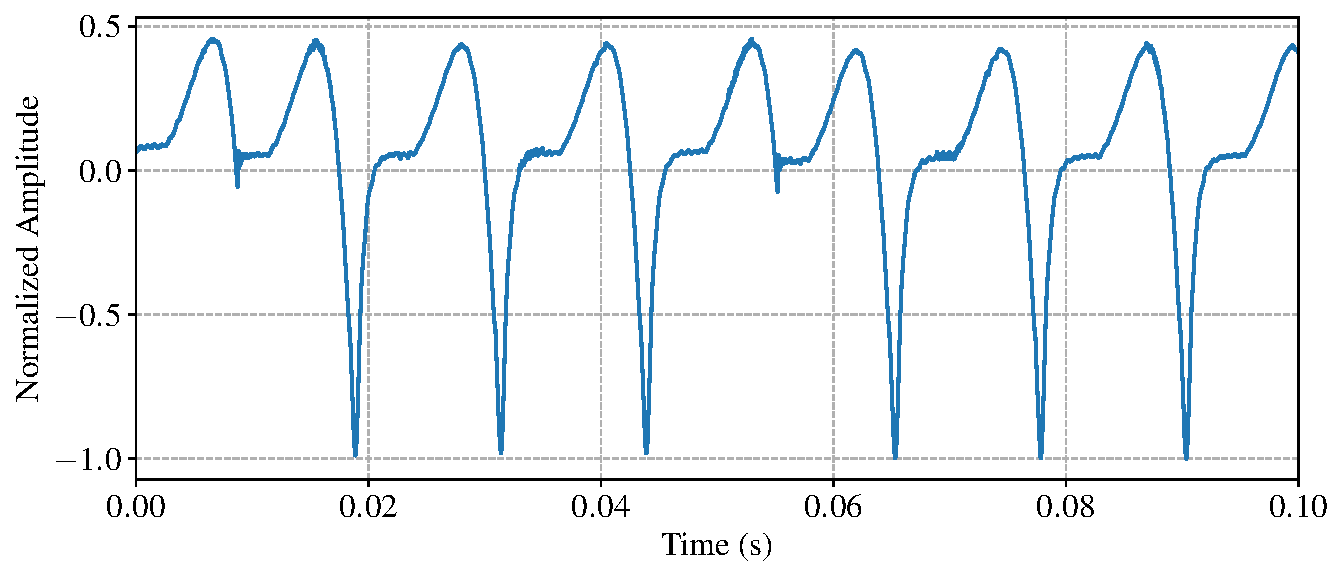
\includegraphics[width = \textwidth]{chapter4/pulseFail.pdf}
    \caption{Failed pulse generation on the STM32 board - 20 harmonics}
    \label{fig:pulseFail}
\end{figure}

Given this, the pulse generation algorithm was then simplified to only compute the pulse waveform once. This was done by calculating a single pulse waveform for a single slightly shorter period than $F_0$ before the main pulse generation loop, and then storing it in memory. The pulse waveform was then copied to the main buffer, and then the index was updated in order to generate the next pulse. This process was repeated until the entire buffer was processed, and then the DMA controller was set to transfer the main buffer back to the audio buffer. This process was repeated until the entire audio buffer was processed, and the audio signal was then output to the audio codec. This process is then the same as shown in Figure \ref{fig:pulseGenFlow}.

\begin{figure}[H]
    \centering
    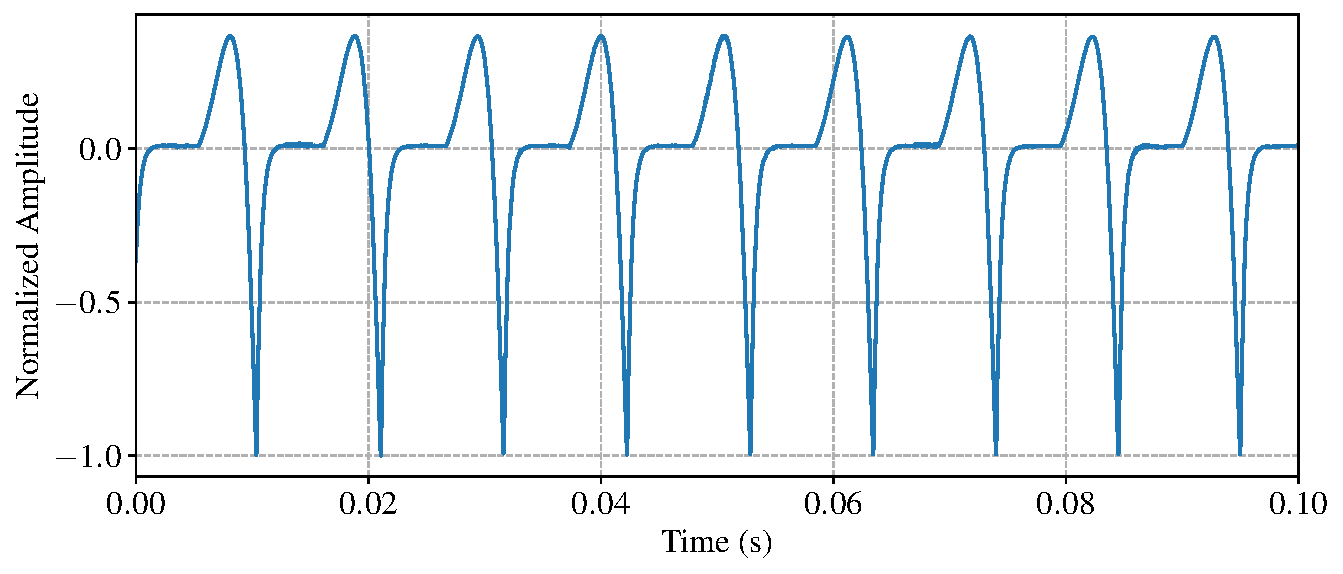
\includegraphics[width=\textwidth]{chapter4/pulseSuccess.pdf}
    \caption{Successful pulse generation on the STM32 board - 200 harmonics}
    \label{fig:pulseSuccess}
\end{figure}

This does come with the disadvantage of having a fixed period pulse waveform, which gets effectively zero-padded according to the desired frequency, and is not an accurate representation of how the glottal flow but does sound natural enough for demonstrating the algorithms shown later on in this work. As mentioned, it also allows for the pulse to be placed at different times, thus varying the pitch of the generated speech signal.

Both results did show however that there were some noises present in the pulse waveform, which were not present in the Python validation results. These were mainly due to the low quality of the audio interface used, which despite having better performance than the one that is found in most desktop motherboards and laptops, did pick up some noise from the power supply. The STM32 also did show some power supply coupling effects that were absent while testing the realtime board on another system.

\section{Fundamental Frequency Envelope}

As is mentioned in Chapters \ref{chap:back} and \ref{chap:sota}, one of the main issues of converting whispered to natural speech is not only the lack of voicing itself, but also the estimation of the fundamental frequency of the speech signal. A fairly realistic method of adding convincing enough prosody to whispered speech is proposed in \cite{ferreiraImplantationVoicingWhispered2016}, where an average fundamental frequency contour was inferred from measuring the average $F_0$ pattern of a portuguese TV journalist at the start of the voiced speech segments.

For the purpose of this work, the function that was used to model the $F_0$ contour was adapted, as shown in Equation (\ref{eq:f0Contour}). In the original paper this curve was defined on a frame-by-frame basis, but for the purposes of this work, the $F_0$ contour is defined as a continuous function of time.

\begin{equation}
    F_0(t) = \phi \left [\hat{F_0} (1 - \alpha t) e^{-\beta t} \sin{\left (\gamma t - \frac{\pi}{3} \right )} - \theta t + \hat{F_0} \right ]
    \label{eq:f0Contour}
\end{equation}

The values for each parameter were then empirically determined in order to have a $F_0$ that sound subtle and natural, as shown in Figure \ref{fig:f0Contour}. The values for each parameter are as follows: $\hat{F_0} = 250$ Hz, $\alpha = 0.13$, $\beta = 0.6$, $\gamma = \pi$, $\theta = 5$ and $\phi = 0.01$. In subsequent, sections this $F_0$ contour will be used to generate the voiced speech signal, and its performance evaluated in the subjective testing.

\begin{figure}[H]
    \centering
    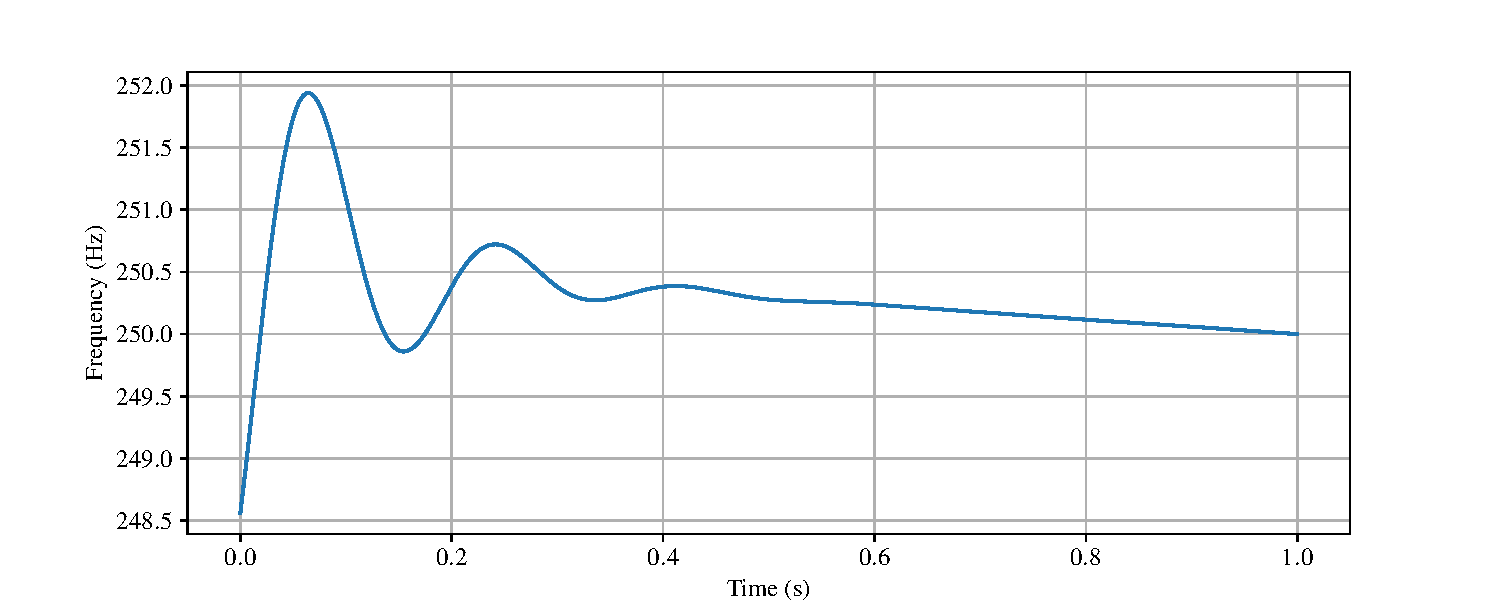
\includegraphics[width=\textwidth]{chapter4/f0Contour.pdf}
    \caption{$F_0$ contour for $\hat{F_0} = 250$ Hz}
    \label{fig:f0Contour}
\end{figure}

While varying the pulse frequency throughout the waveform, it quickly became apparent that the pulse waveform and the way it sounds is quite dependent on the micro-frequency changes that occur within each audio segment. If we only generate each pulse according to the contour's fundamental period at the start of the pulse, even though the length of the pulse is correct, the pulse waveform itself is not. This effect is shown in figure \ref{fig:pulseSpectrum}, where the spectrogram of the pulse waveform is shown for both, to what we'll be referring to as the discrete and continuous $F_0$ frequency pulse generation methods. 

%The discrete pulse generation method is the one where the pulse is generated according to the fundamental frequency at the start of the pulse, and the continuous pulse generation method is the one where the pulse is generated according to the fundamental frequency at each individual sample. It can be seen that the discrete pulse generation method has a lot of spectral leakage, and the pulse waveform spectrum is not as clean as the continuous pulse generation method. This is why the continuous pulse generation method was chosen for the validation implementation of the pulse generation algorithm.

\begin{figure}[H]
    \centering
    \begin{minipage}[H]{0.495\textwidth}
        \centering
        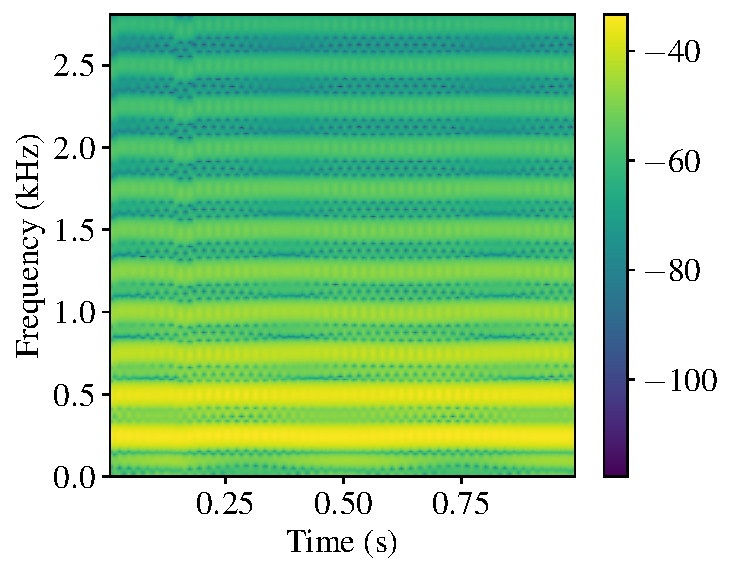
\includegraphics[width=\textwidth]{chapter4/discreteLFspec.pdf}
        \subcaption{}
    \end{minipage}
    \begin{minipage}[H]{0.495\textwidth}
        \centering
        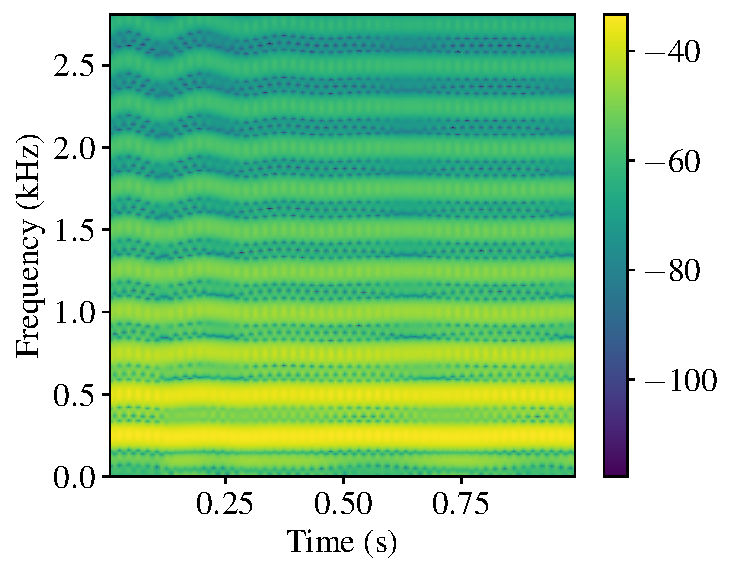
\includegraphics[width=\textwidth]{chapter4/continuousLFspec.pdf}
        \subcaption{}
    \end{minipage}
    
    \caption{LF Pulse spectrogram for a) Discrete pulse $F_0$ b) Continuous pulse $F_0$}
    \label{fig:pulseSpectrum}
\end{figure}

Despite the clear spectral differences between the two methods, and the fact that this difference is audibly perceivable, the discrete pulse generation method was chosen for the real-time implementation, as it is computationally less expensive than the continuous pulse generation method. Moving forward, the discrete pulse generation method will be used for the real-time implementation, and the continuous pulse generation method will be used for the validation of the pulse generation algorithm.

\vfill

\pagebreak


\chapter{Filter Modelling} \label{chap:filt}

After defining the glottal pulse shape and the way it is generated, the next logical step is to model the vocal tract. The vocal tract is modeled as an All-Pole Infinite Impulse Response (IIR) filter, which is used to model the spectral envelope of the speech signal. The filter coefficients are estimated using the Linear Predictive Coding (LPC) analysis, which is a method used to model the spectral envelope of the speech signal. The filter coefficients are then used to synthesize the speech signal by exciting the IIR filter with the pulses. These coefficients are estimated using the autocorrelation method, which first estimates the autocorrelation function of the speech signal using the Weiner-Khintchine theorem, and the coefficients are then estimated using the Levinson-Durbin recursion, which is an efficient algorithm that recursively estimates the filter. 

The filter coefficients are then used to synthesize the speech signal using the IIR filter, which is implemented using the direct form II realization. The filter is then used to synthesize the speech signal using the pulse train generated in the previous chapter, on a pulse-by-pulse basis. This meaning that each pulse is used to excite the filter individually before being concatenated as shown in Chapter \ref{chap:pulseGen}.


\section{LPC Analysis}

As introduced previously in Chapter \ref{chap:back}, the Linear Predictive Coding (LPC) analysis is a method used to model the spectral envelope of a signal. For the purpose of this work, the LPC analysis is used to estimate the filter coefficients of an All-Pole Infinite Impulse Response (IIR) filter that models the vocal tract of the speaker. The LPC analysis is performed on the speech signal $x(n)$, which is divided into overlapping frames of length $N_{\text{frame}} = 512$. The LPC analysis is performed on each frame of the speech signal, and the filter coefficients are estimated for each frame. The filter coefficients are then used to synthesize the speech signal using the IIR filter \cite{hayes1996statistical}.

The LPC analysis is performed using the autocorrelation method, which is depicted in Figure \ref{fig:lpcAnalysis}. The autocorrelation method estimates the autocorrelation function of the speech signal through means of the Weiner-Khintchine theorem.

\begin{figure}[H]
    \centering
    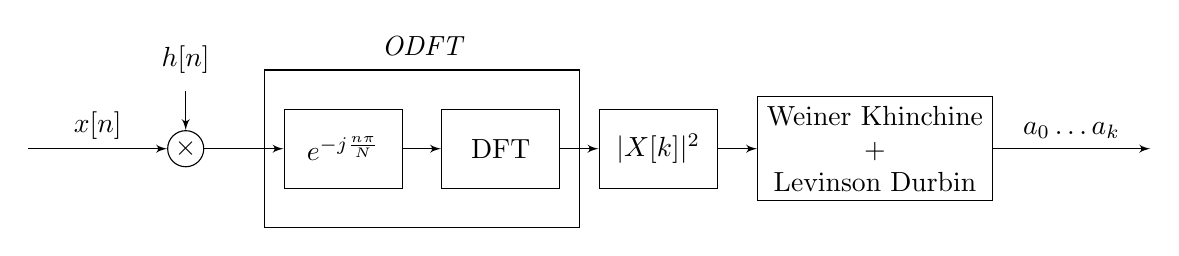
\begin{tikzpicture}[auto, node distance=2cm, >=latex']
        \tikzset{
            block/.style = {draw, rectangle, minimum height=3em, minimum width=3em},
            sum/.style = {draw, circle, node distance=1cm},
            input/.style = {coordinate},
            output/.style = {coordinate},
            pinstyle/.style = {pin edge={to-,thin,black}}
        }
        % ODFT 
        \draw (3,-1) rectangle ++(4, 2);
        \node at (5, 1.3) {\it ODFT};

        \node [coordinate] (input) {};
        \node [circle, draw, inner sep = 1pt, right of=input] (mult) {$\times$};
        \node [coordinate, above =0.5cm of mult] (win) {};
        \node [above = 0.1cm of win] (window) {$h[n]$};
        \node [rectangle, minimum width = 1.5cm, minimum height = 1cm,draw, right of = mult] (exp) {$e^{-j\frac{n\pi}{N}}$};
        \node [rectangle, minimum width = 1.5cm, minimum height = 1cm, draw, right of = exp] (dft) {DFT};
        \node [rectangle, minimum width = 1.5cm, minimum height = 1cm, draw, right of = dft] (psd) {$|X[k]|^2$};
        \node [rectangle, minimum width = 1.5cm, minimum height = 1cm, draw, align=center, right = 0.5cm of psd] (lev) {Weiner Khinchine \\ + \\ Levinson Durbin};
        \node [coordinate, right = 2cm of lev] (output) {};
        
        \draw [->] (input) -- node {$x[n]$} (mult);
        \draw [->] (win) -- (mult);
        \draw [->] (mult) -- (exp);
        \draw [->] (exp) -- (dft);
        \draw [->] (dft) -- (psd);
        \draw [->] (psd) -- (lev);
        \draw [->] (lev) -- node {$a_0 \dots a_k$} (output);
    \end{tikzpicture}
    \caption{LPC Analysis Signal Flow Graph}
    \label{fig:lpcAnalysis}
\end{figure}

\subsection{ODFT}

As the filter coefficients are determined in the frequency domain, by means of the Odd Discrete Fourier Transform (ODFT) \cite{ferreiraAccurateEstimationODFT2001}. The Odd Fourier transform is what is referred to as a partial transform, which takes advantage of the property that for a given signal $x(n)$ the Nth order DFT of the signal is real and even, i.e. $X(k) = X(N-k)$, and thus it is only necessary to compute the odd part of the DFT \cite{bellanger2024digital}.

This property is used to both reduce the computational complexity of the DFT algorithm, by only computing the odd part of the DFT of the signal and to achieve perfect signal reconstruction \cite{ferreiraAccurateEstimationODFT2001} when no processing is done between the input and output. Firstly, the transform is computed by multiplying the signal $x(n)$ by a window function $h(n)$, in this case a shifted Sinusoidal window, as shown in Equation \ref{eq:windowFunc}.

\begin{equation}
    h[n] = \sin \left ( \frac{\pi(n+0.5)}{N} \right )
    \label{eq:windowFunc}
\end{equation}

Next, this operation is followed by then multiplying the result by the exponential function $e^{-j\frac{n\pi}{N}}$. The ODFT is then finally computed using a standard FFT algorithm, and the power spectral density of the speech signal is estimated resulting in what is sometimes referred to as the Power ODFT \cite{goncalvesVozeamentoSinteticoVoz2023}.



%The ODFT is a method used to estimate the Discrete Fourier Transform (DFT) of a signal using the autocorrelation function of the signal. The ODFT is used to estimate the DFT of the speech signal $x(n)$, which is then used to estimate the filter coefficients of the IIR filter. The ODFT is performed on the speech signal $x(n)$, which is multiplied by a window function $sinW(n)$, and then multiplied by the exponential function $e^{-j\frac{n\pi}{N}}$. The ODFT is then computed using the DFT algorithm, and the power spectral density of the speech signal is estimated. The Weiner-Khintchine theorem is then used to estimate the autocorrelation function of the speech signal, which is then used to estimate the filter coefficients using the Levinson-Durbin recursion.

\subsection{Levinson-Durbin algorithm}

The Levinson-Durbin recursion is an efficient algorithm that recursively estimates the filter coefficients by minimizing the prediction error \cite{yuMultistageLevinsonDurbinAlgorithm2002}. The filter coefficients are estimated by solving the Toeplitz system of Equations (\ref{eq:yulewalker}) presented in Chapter \ref{chap:back}, which require the autocorrelation coefficients of the speech signal to first be determined by means of the Weiner-Khintchine theorem. The algorithm has a time complexity of $O(n^2)$ \cite{hayes1996statistical}, whereas other methods of solving the required system of equations, say through a least squares approach, would have a time complexity of $O(n^3)$. 
\begin{comment}
A general description of the Levinson-Durbin recursion is as follows \cite{yuMultistageLevinsonDurbinAlgorithm2002}:

\begin{enumerate}
    \item Determine the autocorrelation sequence \( r[\tau] \)
    \item Initialize \( E_0 = r[0] \), \( a_0 = 1 \)
    \item For \( i = 1, 2, \ldots, p \):
    \begin{enumerate}
        \item Calculate the reflection coefficient (also known as the Parcor coefficient):
        \[
        k_i = \frac{r[i] - \sum_{j=1}^{i-1} a_j^{(i-1)} r[i-j]}{E_{i-1}}
        \]
        \item Update the prediction error:
        \[
        E_i = (1 - k_i^2) E_{i-1}
        \]
        \item Update the coefficients:
        \[
        a_i = a_{i-1}^{(i-1)} + k_i \left( 1 - \sum_{j=1}^{i-1} a_j^{(i-1)} \right)
        \]
        \item For \( j = 1, 2, \ldots, i-1 \):
        \[
        a_j^{(i)} = a_j^{(i-1)} - k_i a_{i-j}^{(i-1)}
        \]
    \end{enumerate}
\end{enumerate}
\end{comment}

The Levinson-Durbin recursion is implemented in Python in listing \ref{lst:levinsonPy}, and is written taking advantage of the vector and matrix processing capabilities that are provided by NumPy. The function \texttt{levinson()} takes as input the autocorrelation coefficients $r$ of the speech signal and the filter order $N$, and returns the filter coefficients $a[k]$, the prediction error $E$, and the reflection coefficients $k$.

Besides the calculation of the $a_k$ filter denominator coefficient, another important metric is that of the $b_0$ filter gain coefficient. This coefficient is calculated as the square root of the prediction error $E$. This is called the autocorrelation matching property, and it is used to ensure that the energy of input signal is the same as the energy of the filter which is given by its first autocorrelation coefficient \cite{hayes1996statistical}.

\begin{lstlisting}[language=Python, style=mystyle, caption={Levinson Durbin Recursion in Python}, label={lst:levinsonPy}]
    def levinson(r, N):
        k = np.zeros(N+1) # Reflection coefficients
        A = np.zeros(N+1) # Prediction filter coefficients
        A[0] = 1.0
        E = np.real(r[0]) # Prediction error
    
        # Levinson-Durbin recursion
        for i in range(1, N+1):
            lambda_ = -np.dot(r[1:i+1], A[i-1::-1]) / E
            A[1:i+1] += lambda_ * A[i-1::-1]
            E *= (1.0 - lambda_ * lambda_)
            k[i] = -lambda_  # Reflection coefficient is the negation of lambda_
        
        return A, E, k[1:]
    \end{lstlisting}

Before applying the Levinson-Durbin algorithm for the estimation of the filter coefficients, the autocorrelation coefficients of the speech signal must be estimated. The autocorrelation coefficients are estimated using the Weiner-Khintchine theorem, which states that the autocorrelation function of a signal is the inverse Fourier transform of the power spectral density of the signal \cite{hayes1996statistical, engelberg2006random}. The power spectral density of the speech signal is estimated using the ODFT, and the autocorrelation coefficients are then estimated using the inverse Fourier transform of the power spectral density. For an input signal $x[n]$ with a corresponding ODFT of $X[k]$, the autocorrelation coefficients $r[\tau]$ are estimated using the Weiner-Khintchine theorem as shown in Equation \ref{eq:wienerkhintchine}, where $\mathcal{F}^{-1}$ represents the inverse ODFT operation and $PSD[k]$ is the Power Spectral Density corresponding to signal $x[n]$.

\begin{equation}
    r[\tau] = \mathcal{F}^{-1}\{|X[k]|^2\} = \mathcal{F}^{-1}\{PSD[k]\}
    \label{eq:wienerkhintchine}
\end{equation}

\subsubsection{Realtime Implementation}

The Levinson-Durbin recursion is implemented in C in listing \ref{lst:levinsonC}. The function \texttt{levinson()} takes as input the autocorrelation coefficients $r$ of the speech signal and the filter order \texttt{n}, and returns the filter coefficients \texttt{a}, the prediction error \texttt{e}, and the reflection coefficients \texttt{k}.

\begin{lstlisting}[language=C, caption={Levinson Recursion in C}, label={lst:levinsonC}]
void levinson(float32_t* r, uint16_t n_len, float32_t* a, float32_t* e){
    float32_t lambda[n_len + 1];
    a[0] = 1.0;
    *e = r[0];

    float32_t lambdaSum, temp;
    for (size_t i = 1; i <= N; i++){
        lambdaSum = 0.0f;

        for (size_t j = 1; j <= i; j++)
            lambdaSum += a[j] * r[i - j];

        lambda[i] = -lambdaSum / (*e);

        for (size_t j = 1; j <= i / 2; j++){
            temp = a[j] + lambda[i] * a[i - j];
            a[i - j] += lambda[i] * a[j];
            a[j] = temp;
        }

        a[i] = lambda[i];
        (*e) = (*e) * (1 - lambda[i] * lambda[i]);
    }

    return;
}
\end{lstlisting}


\section{Filter Realization}

The standard formula for the IIR filter response in the z-domain is given by Equation (\ref{eq:typeIIfilter}). The filter coefficients $a_k$ and $b_0$ are determined by the LPC analysis, and the filter order $N$ is determined by the number of poles in the LPC analysis.

\begin{equation}
    H(z) = \frac{B(z)}{A(z)} = \frac{b_0 + \sum_{k=1}^{N}b_k z^{-k}}{1 + \sum_{k=1}^{N}a_k z^{-k}}
    \label{eq:typeIIfilter}
\end{equation}

In order to implement the IIR filter, we need to choose a realization structure. The direct form II realization is chosen for its simplicity and ease of implementation, as only single delay line $w(n)$ is needed and no reflection coefficients need to be computed \cite{jackson1996digital}. The signal flow chart for this type of realization is shown in Figure \ref{fig:directTypeII} for a second order system. Considering the input signal $x(n)$ and the output signal $y(n)$, the direct form II realization of the IIR filter can be described by the following difference equations in \ref{eq:directTypeII}.

\begin{equation}
    \begin{cases}
        w(n) = x(n) - \sum_{k=1}^{N} a_k w(n-k) \\
        y(n) = \sum_{k=0}^{N} b_k w(n-k) = b_0 w(n)
    \end{cases}
    \label{eq:directTypeII}
\end{equation}


\begin{figure}[H]
    \centering    

    % direct type II IIR realization tikz picture
    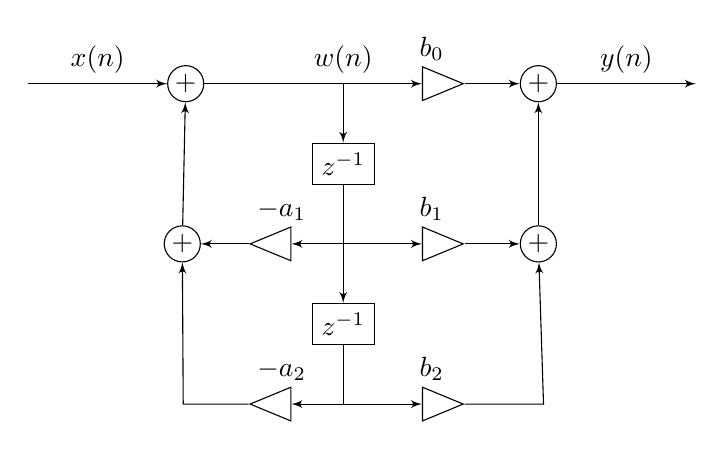
\begin{tikzpicture}[auto, node distance=2cm,>=latex']
        % Nodes
        \node [coordinate] (input) {};
        \node [circle, draw, inner sep=1pt, right of=input] (sum1) {$+$};
        \node [coordinate, right of=sum1, label = above:$w(n)$] (delay0) {};
        \node [rectangle, draw, below = 0.75cm of delay0] (delayLine1) {$z^{-1}$};
        \node [coordinate, below=0.75cm of delayLine1] (delay1) {};
        \node [rectangle, draw, below= 0.75cm of delay1] (delayLine2) {$z^{-1}$};
        \node [coordinate, below=0.75cm of delayLine2] (delay2) {};    
        \node [isosceles triangle, draw, right=1cm of delay0, label = above:$b_0$] (b0) {};
        \node [isosceles triangle, draw, right=1cm of delay1, label = above:$b_1$] (b1) {};
        \node [isosceles triangle, draw, right=1cm of delay2, label = above:$b_2$] (b2) {};
        \node [isosceles triangle, rotate=180, draw, left=1.2cm of delay2, label = below:$-a_2$] (a2) {};
        \node [isosceles triangle, rotate=180, draw, left=1.2cm of delay1, label = below:$-a_1$] (a1) {};
        \node [circle, draw, inner sep=1pt, left=1.15cm of a1] (sum2) {$+$};
        \node [circle, draw, inner sep=1pt, right=0.7cm of b1] (sum3) {$+$};
        \node [circle, draw, inner sep=1pt, right=0.7cm of b0] (sum4) {$+$};
        \node [coordinate, right of = sum4] (output) {};

        % Connections
        \draw [->] (input) -- node {$x(n)$} (sum1);
        \draw [-] (sum1) -- (delay0);
        \draw [->] (delay0) -- (delayLine1);
        \draw [->] (delay0) -- (b0);
        \draw [-] (delayLine1) -- (delay1);
        \draw [->] (delay1) -- (b1);
        \draw [->] (delay1) -- (a1);
        \draw [->] (delay1) -- (delayLine2);
        \draw [-] (delay2) -- (delayLine2);
        \draw [->] (a1) -- (sum2);
        \draw [->] (a2) -- ++(-1.25cm, 0) -- (sum2);
        \draw [->] (delay2) -- (a2);
        \draw [->] (delay2) -- (b2);
        \draw [->] (sum2) -- (sum1);
        \draw [->] (b0) -- (sum4);
        \draw [->] (b1) -- (sum3);
        \draw [->] (sum4) -- node {$y(n)$} (output);
        \draw [->] (sum3) -- (sum4);
        \draw [->] (b2) -- ++(1.42cm, 0) -- (sum3);
    \end{tikzpicture}
    
    \caption{Direct-Type-II IIR Filter Signal Flow Graph - 2nd order}
    \label{fig:directTypeII}
\end{figure}

\subsection{Realtime Implementation}

The structure represented in figure \ref{fig:directTypeII} is, obviously, simplified and in our implementation its order is determined by the number of poles in the LPC analysis. It is also worth to note that all filter numerator coefficients besides $b_0$ are all null. Therefore, there is room to reduce the computational complexity of the filter.

\begin{lstlisting}[language=C, style=mystyle]
void iirDirectTypeII(float32_t* in, float32_t* out, int len, float32_t b0, float32_t* a, int coeffLen){
    // set output to all zeros
    memset(out, 0.0f, len);
    
    // variable length arrays are allowed in C99
    float32_t w[coeffLen]; // delay line initialized to all zeros
    memset(w, 0.0f, coeffLen);

    for (int32_t i = 0; i < len; i++){
        // First difference equation is to determine w[n] from the denominator
        w[0] = in[i];
        for(int32_t j = 1; j < coeffLen; j++) // compute the output delay line
            w[0] -= a[j] * w[j];

        // Second difference equation is simplified as there is only b0
        out[i] = b0 * w[0];

        // Shift delay line
        for (int32_t j = coeffLen - 1; j > 0; j--)
            w[j] = w[j - 1];
    }

    return;
}    
\end{lstlisting}


\section{Spectral Tilt Compensation}

One important aspect of the vocal tract filter model is that of the spectral tilt compensation. Tilt compensation is a technique used to adjust the gain of the filter in order to compensate for what is called the spectral tilt of the speech signal \cite{ferreira2018on}. The spectral tilt of the speech signal is a characteristic of the speech signal that is related to the power spectral density of the glottal source signal across the frequency spectrum. It is an important characteristic of the speech signal that can affect the perceived naturalness and quality of the synthesized speech signal. Thus, compensation is required in order to adjust the frequency response of the filter that is inferred from the whispered signal as to improve the quality of the synthesized speech signal.

Using the LF glottal derivate model harmonics that were obtained in Chapter \ref{chap:pulseGen}, the spectral tilt of the glottal pulse can be estimated for any given fundamental frequency. This spectral tilt of the glottal pulse is then used to estimate the spectral tilt of the synthesized speech signal, given the target fundamental frequency. In Figure \ref{fig:tiltGain} we can see the magnitude of the glottal pulse frequency response and how it can be seen rolling off in the higher frequencies. 

\begin{figure}[H]
    \centering
    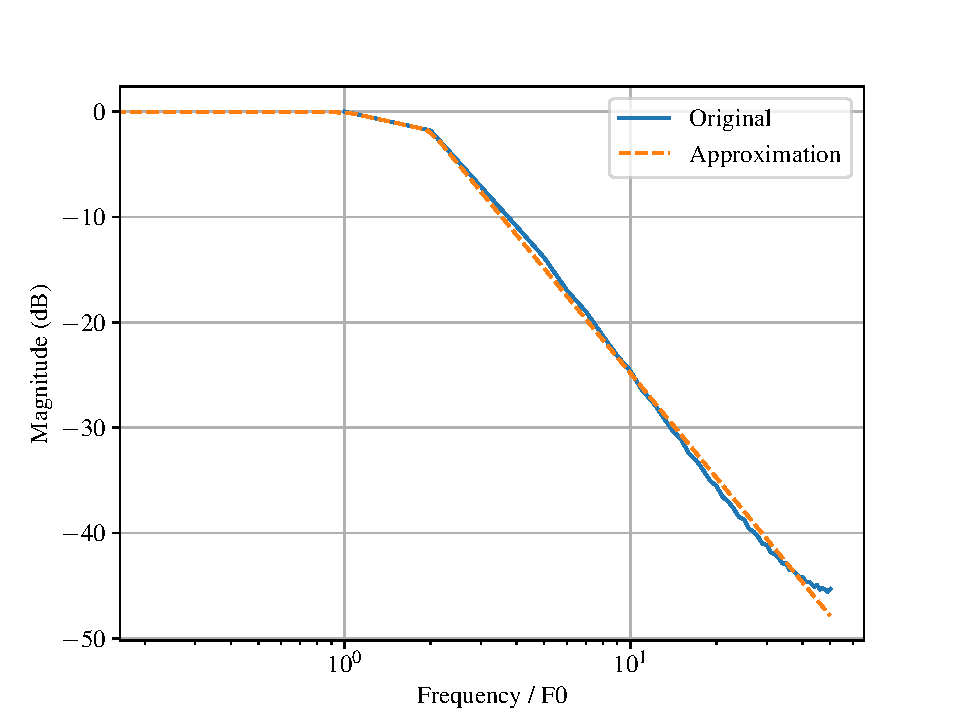
\includegraphics[width = 0.8\textwidth]{chapter5/glottalPulseTiltGain.pdf}
    \caption{Glottal Pulse Spectral Tilt}
    \label{fig:tiltGain}
\end{figure}

In \cite{ferreira2018on}, Ferreira establishes that the spectral tilt compensation can be approximated by a piecewise function consisting of 3 linear segments in the log-frequency domain. The first segment is a flat response, the second segment is a linear increase in gain, and the third segment is a further linear decrease in gain. In this case, the pulse gain is modelled in the following way:

\begin{equation}
    \begin{cases}
        1.0 & \text{if } f < f_0 \\
        b_1 - m_1f & \text{if } f/f_0 \in [1, 2] \\
        b_2 - m_2f & \text{otherwise}
    \end{cases}
\end{equation}

These values are then precomputed at the start of the program and stored in an array that is multiplied to each PSD before doing the IODFT and the Levinson-Durbin recursion. This is done in order to avoid having to do the same calculations over and over for each frame of the speech signal. It is relevant to point out that this function does obviously vary with the fundamental frequency of the glottal pulses, as can be seen in Figure \ref{fig:tiltCompensation}. This effect is noticeable for large variations of $F_0$, but it was deemed as small enough for the microvariations of $F_0$ which most likely do not warrant for this compensation to be computed individually for each pulse period.

\begin{figure}[H]
    \centering
    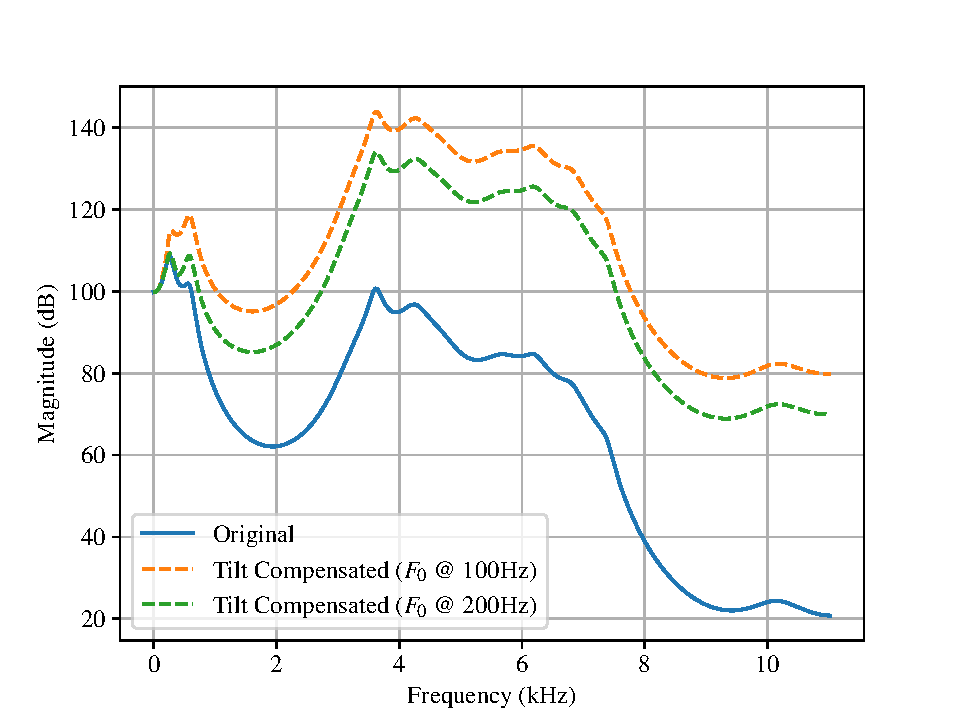
\includegraphics[width = 0.8\textwidth]{chapter5/vowelTiltCompensation.pdf}
    \caption{Comparison of uncompensated and tilt compensated spectral envelopes}
    \label{fig:tiltCompensation}
\end{figure}

\section{Vowel Synthesis}

In order to both validate the filter realization and the tilt compensation, synthetic vowels were generated from a set of vowel spectral envelopes that were determined in a similar fashion to \cite{ferreiraMismatchPhaseStructure2024}, which in turn is based on the LPC estimation mechanism of Figure \ref{fig:lpcAnalysis}. These were inferred before from voiced samples of a very high pitch female voice.

Utilizing the LPC modelling mechanism along with the tilt compensation, filters were generated from each of the vowel spectral envelopes, which were then excited using the LF pulse train generated in Chapter \ref{chap:pulseGen}, following the $F_0$ contour that was established in the same chapter in Equation (\ref{eq:f0Contour}). As determined in previous research on the DyNaVoiceR project \cite{oliveiraModelizacaoFiltroTrato2020} the filter order that was utilized for modelling the vocal tract was $N_{LPC} = 22$, which allows for up to 11 formant frequencies to be represented. Figure \ref{fig:vowelTemplates} shows the spectral envelopes of each of the tonic vowels of European Portuguese, which were used to generate the synthetic vowels.

\begin{figure}[H]
    \centering
    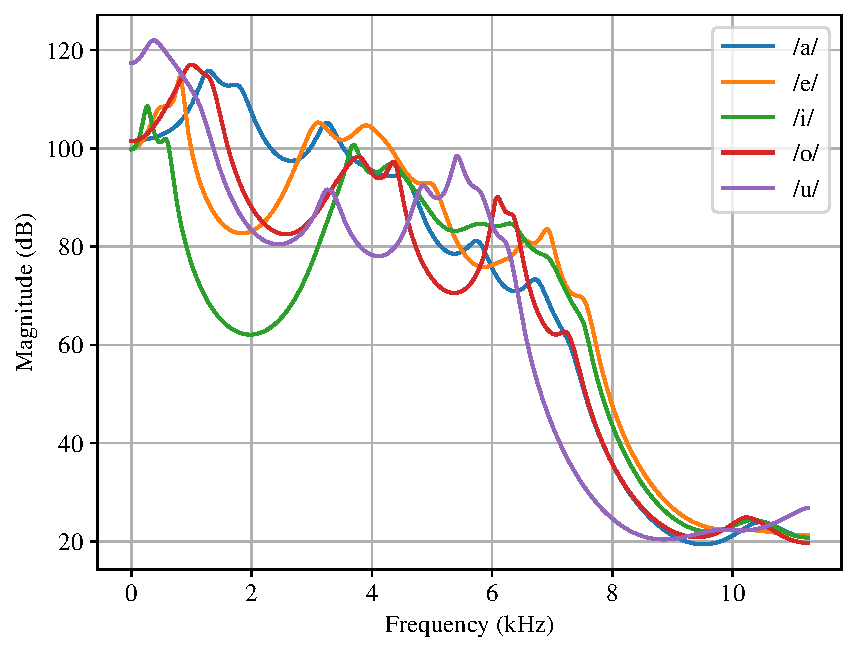
\includegraphics[width=0.7\textwidth]{chapter5/vowelsTemplates.pdf}
    \caption{Spectral envelopes for each tonic vowel of EP}
    \label{fig:vowelTemplates}
\end{figure}

From these spectral envelopes the models are generated using the same LPC analysis mechanism in the previous sections of this chapter. The filters are then excited using a pulse train generated from the LF glottal pulse model that is shown in Chapter (\ref{chap:pulseGen}). The implementation in C can be seen in listing \ref{lst:vowelSynth}, where CMSIS function are taken advantage of in order to speed up not only the computations, as they are optimized for the ARM Cortex-M7 core Neon instructions, but also speed up the development process. 

Regarding the code snippet in \ref{lst:vowelSynth}, the PSD of each vowel was already in memory in the variable \texttt{psd} such that the IODFT can be computed directly, and then Levinson-Durbin recursion is then applied to the reflection coefficients, without analyzing any of the input signal frames coming from the DMA. This is done just for the sake of simplicity, as the main goal of this chapter is to show the filter realization and the tilt compensation mechanism. Figure \ref{fig:vowelPulses} shows the filtered pulses that were obtained in real-time using the spectral envelopes template of the /a/ vowel. 

\mybreak 

\begin{figure}[H]
    \centering
    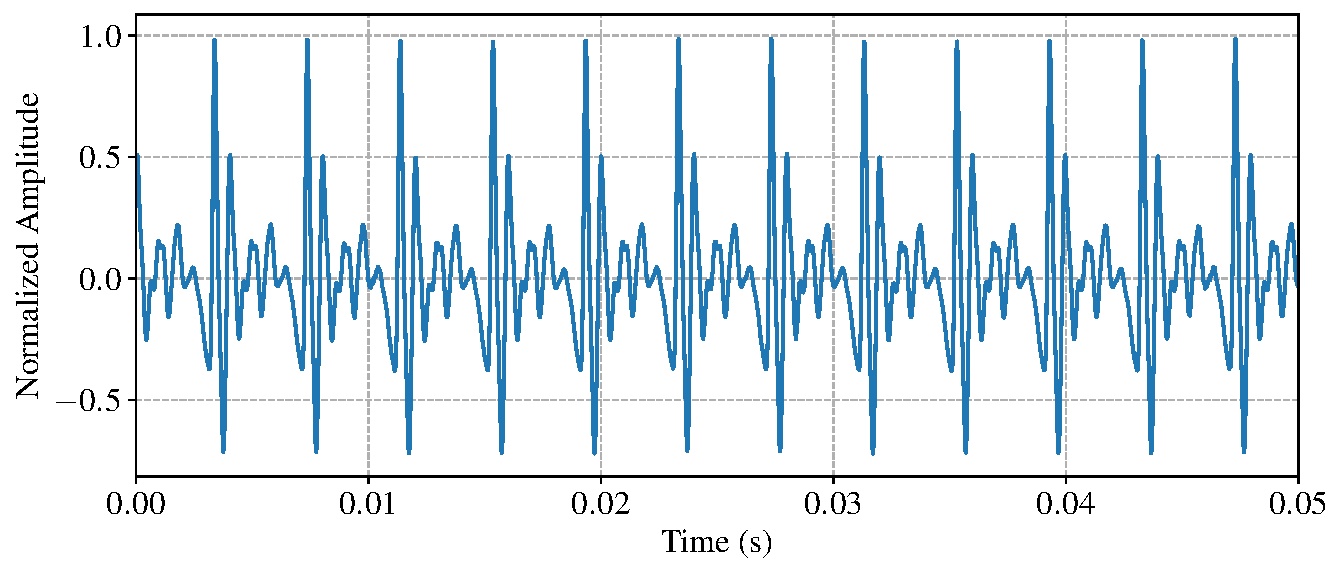
\includegraphics[width=0.9\textwidth]{chapter5/filteredPulses.pdf}
    \caption{Filtered Pulses in realtime}
    \label{fig:vowelPulses}
\end{figure}

Furthermore, the spectral envelopes of the synthetic vowels were also analyzed in order to validate the filter realization and the tilt compensation, in both the Python and realtime environments. Figure \ref{fig:vowelSpectrum} shows the spectral envelope of the ideal synthesized vowel and the synthetic vowel generated using the filter realization and the tilt compensation. The synthetic vowel closely resembles the ideal vowel, which validates the filter realization and the tilt compensation mechanism. 

It becomes clear although that the STM32 is not able to generate the same quality of the synthetic vowels as the Python implementation, which is expected due to not only the computational limitations of the microcontroller that have been exposed in the previous chapter, but also due to the fact that there is a real noise floor on the microcontroller's audio output which is obviously not present in the validation environment.

\begin{figure}[H]
    \centering
    \begin{minipage}[H]{0.495\textwidth}
        \centering
        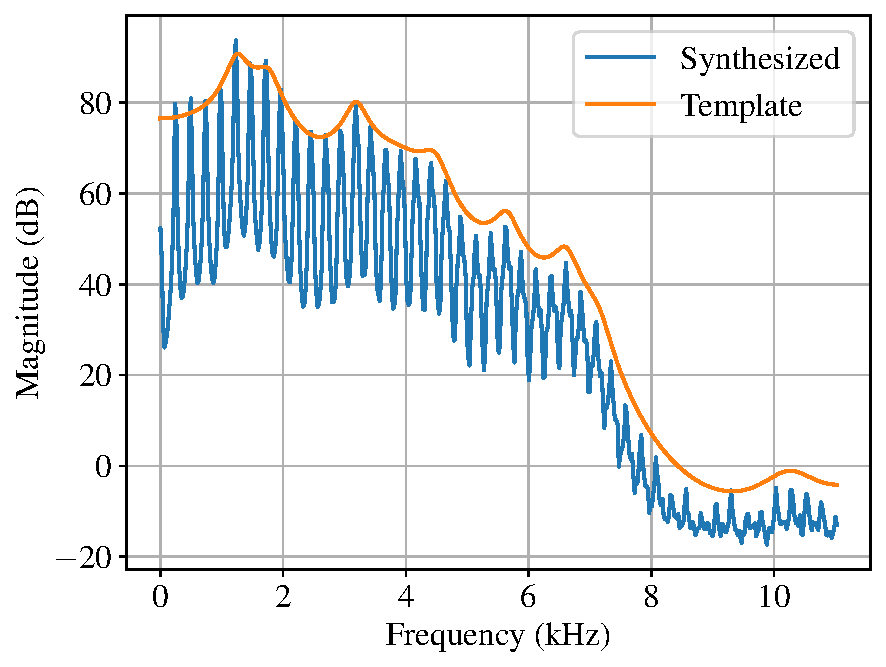
\includegraphics[width=\textwidth]{chapter5/idealSpectrum.pdf}
        \subcaption{}
    \end{minipage}
    \begin{minipage}[H]{0.495\textwidth}
        \centering
        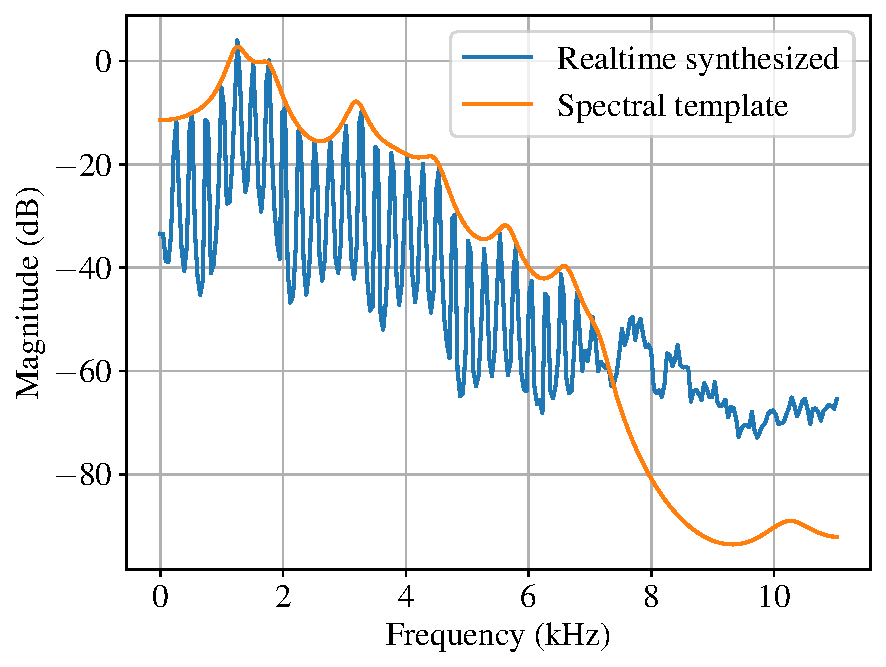
\includegraphics[width=\textwidth]{chapter5/realtimeSpectrum.pdf}
        \subcaption{}
    \end{minipage}
    \caption{Spectral envelope of the ideally synthesized vowel (a) and the realtime synthesized vowel (b)}
    \label{fig:vowelSpectrum}
\end{figure}



%\vspace*{12mm}

\chapter{Overlap Add Reconstruction of Voiced Speech} \label{chap:overlapAdd}

In this next chapter, we will describe and discuss the proposed system architecture for the overlap add reconstruction of voiced speech. Besides that, both the whisper activity detection and speech segmentation algorithms that are used in the proposed system for silence detection and Voiced/Unvoiced decisions are introduced and discussed.

The system is meant to take in whispered speech as input, and output a reconstructed voiced speech signal, by first utilizing the LPC filtering mechanism presented in Chapter \ref{chap:filt}, and exciting that with both synthetic pulses, for the case of voiced speech segments and noise in the case of unvoiced regions. 

\section{Proposed System Architecture}

The diagram for the complete system architecture can be seen in Figure \ref{fig:systemDiagram}. It works by first taking in input frames which are 512 samples long, and then applying a 50\% overlap to these frames, along with the previous frame in order to obtain a 1024 sample windowed frame. Then the PSD of this frame is computed through the ODFT, as shown in the previous chapter, which gets mixed with PSD that was obtained in the previous frame. This is done in order to obtain a smooth transition between filters across frames. This mechanism can be visualized in Figure \ref{fig:pulseMap}, where according to the relative position of each pulse within the current frame $\alpha_k$, a new filter is created by mixing the current frame's PSD with the one obtained in the previous frame. This is done by means of a linear interpolation between the two PSDs, as shown in Equation (\ref{eq:psdInterpolation}).

\begin{equation}
    PSD_{pulse}[k] = (1-\alpha_k) PSD_{j-1}[k] + \alpha_k PSD_j[k]
    \label{eq:psdInterpolation}
\end{equation}

From this new PSD, and using the same LPC analysis mechanism as in the previous chapter, a new filter $H_j[k]$ is obtained, that is only used for the pulse in question. This newly generated filter is then used to filter the pulse in the time domain, and the result is then added to the output at \texttt{mainBuff[n]}, using the same overlap logic that was used in Chapter \ref{chap:pulseGen} for the pulse generation and concatenation. 

For mixing the PSDs of the current and previous frames, the mixing factor $\alpha_k$ is defined as shown in Equation (\ref{eq:alphaDef}), where $lastPulsePos$ is the current sample number and $N_2$ is the total number of samples in the frame.

\begin{equation}
    \alpha_k = \frac{\text{lastPulsePos}}{N_2}
    \label{eq:alphaDef}
\end{equation}

Before computing the filter, tilt compensation is applied to the PSD, as per the method described in the previous chapter. This tilt factor is precomputed beforehand at startup and is applied equally to all interpolated PSDs, as the changes in the generated pulse frequencies are not significant enough to warrant a per-pulse tilt compensation. 

\begin{figure}[H]
    \centering
    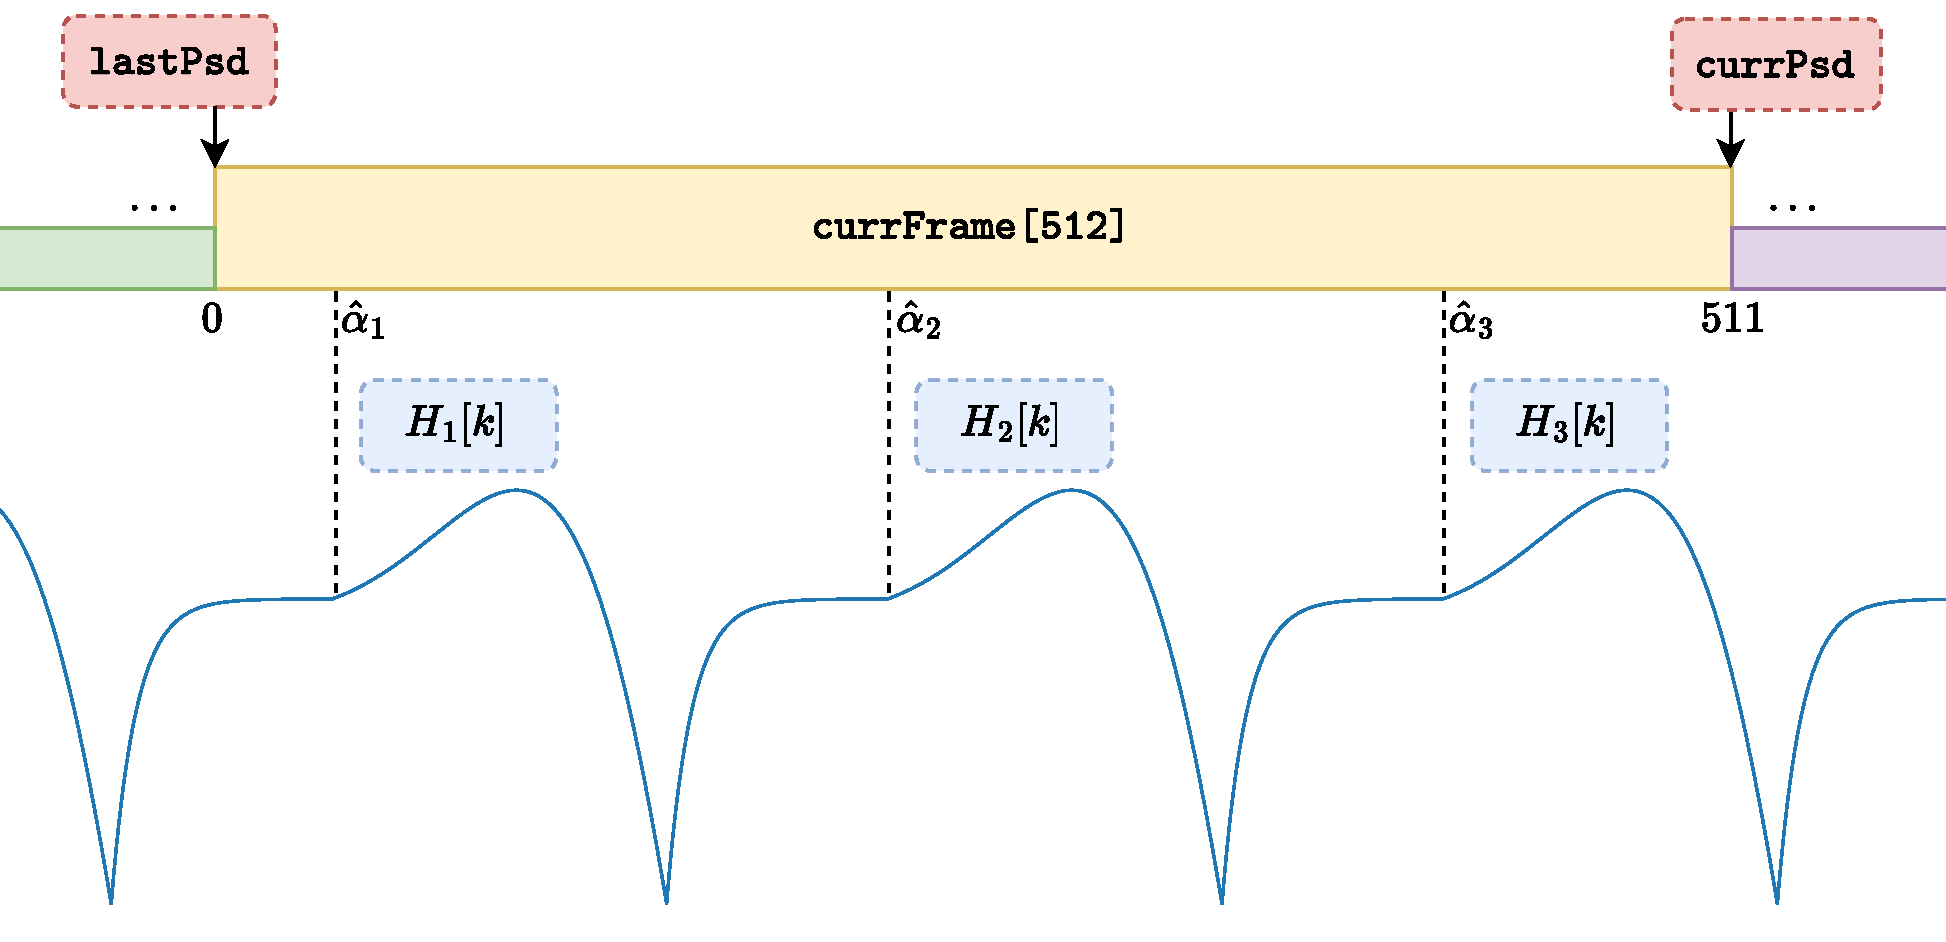
\includegraphics[width=0.9\textwidth]{chapter6/pulseMap.pdf}
    \caption{Individual pulse filtering mechanism}
    \label{fig:pulseMap}
\end{figure}

The system also includes a mechanism for whispered activity detection and another for speech segmentation, which are used to determine the activity of the signal and how to treat each frame in terms of whether it is voiced or unvoiced. These two mechanisms are also used to determine the fundamental frequency of the voiced segments of the signal, by triggering the $f_0(t)$ contour to be applied to the voiced segments of the signal. This contour is also reset whenever there are either silent or unvoiced speech segments. Hopefully this approach improves the prosody of the synthesized speech.

In order to mix both the LF pulse and noise excitation sources in the time domain, a $\beta$ factor is used to determine the relative gain of each source. This factor is determined by the mapping of the centre of gravity to a value between 0 and 1, as we will show in the next sections.

\begin{figure}[H]
    \centering
    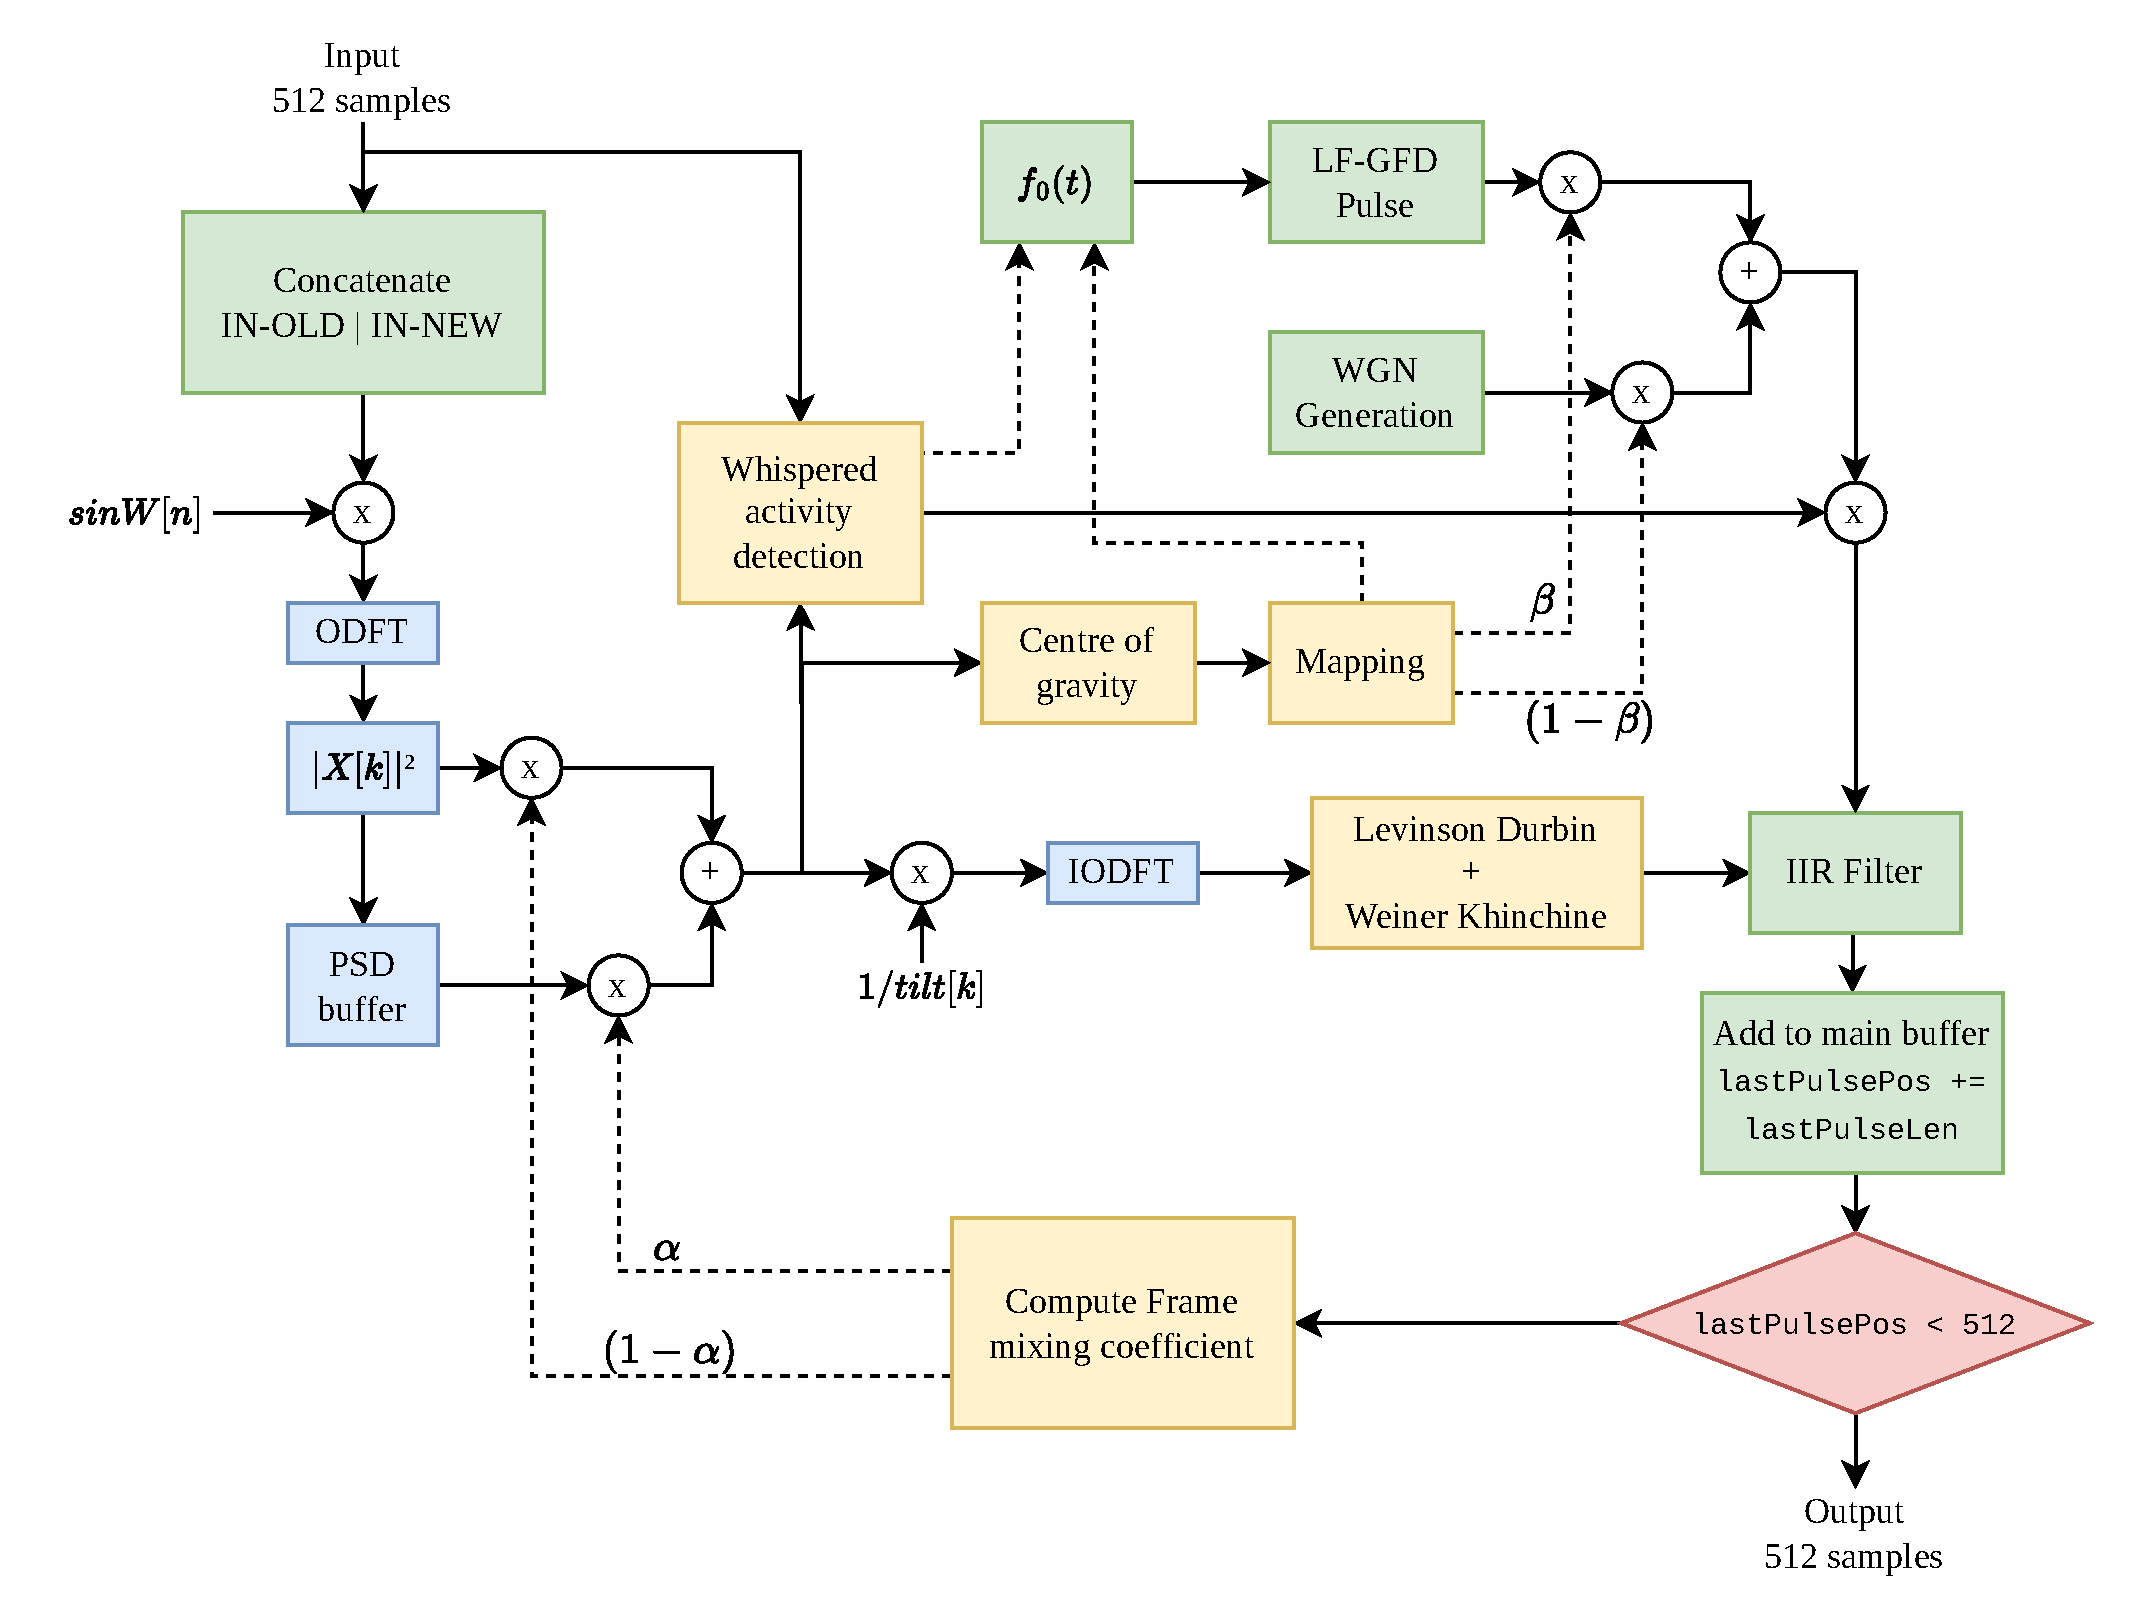
\includegraphics[width=1.0\textwidth]{chapter6/systemDiagram.pdf}
    \caption{Complete System Diagram}
    \label{fig:systemDiagram}
\end{figure}


\section{Whisper Activity Detection}

Similarly to what as proposed by Sharifzadeh et.al in \cite{sharifzadehReconstructionNormalSounding2010}, a modified version of the G.729 whisper activity detection algorithm, as shown in \cite{beritelliPerformanceEvaluationComparison2002}, was utilized for the detection of actual whispered speech in the input signal. This is of course necessary such that the $F_0$ contour can be properly applied to the voiced segments of the signal and such that the voicing decisions are only done on the segments that have actual speech.

In this case, each speech segment is determined as active or idling, by means of both its energy and its zero crossing rate. Three thresholds $\zeta_1$, $\zeta_2$ and $\zeta_{zcr}$, are used to determine the activity of the signal, and the algorithm is as follows, where the energy for a given frame $x[n]$ is given by $E$ and its zero crossing rate is given by $\gamma$:

\begin{equation}
    \text{Activity} = 
    \begin{cases}
        1.0 & \text{if } E > \zeta_2 \\
        0.0 & \text{if } E < \zeta_1 \\
        \frac{\text{sign}{(\gamma - \zeta_{zcr})} + 1}{2} & \text{otherwise}
    \end{cases}
\end{equation}

In the original paper, it is mentioned that the 3 thresholds are adaptive although no reference is made to the way in which these are adapted. As such, it was established that the thresholds would be set empirically on a speaker-by-speaker basis. The way these were set will be discussed in the next section where the results are taken. Figure \ref{fig:g279detection} shows the whispered activity algorithm in action upon a whispered signal.

\begin{figure}[H]
    \centering
    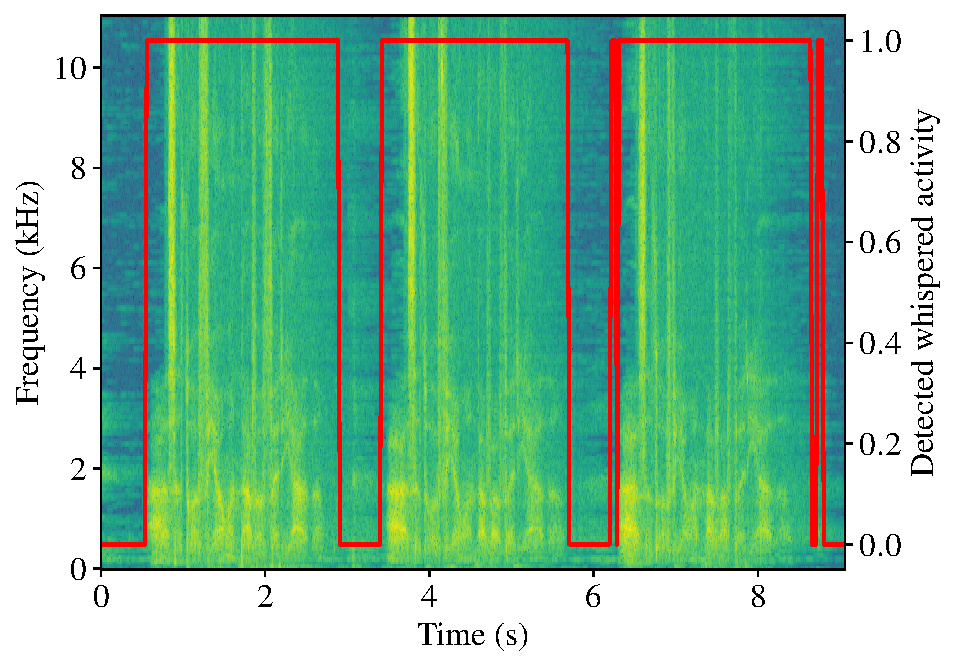
\includegraphics[width=0.8\textwidth]{chapter6/g279detection.pdf}
    \caption{\centering Whispered Detection algorithm applied to a whispered signal - {\it "A asa do avião andava avariada"}}
    \label{fig:g279detection}
\end{figure}

It is worth noting that the previous figure constitutes a best case scenario where all the thresholds are manually set to minimize false activity detection, it is although apparent that the algorithm is not perfect and that there are still some false positives and negatives, particularly when breathing sounds become particularly loud in between whispered utterances. This is to be expected as the algorithm is quite simple and does not take into account the actual content of the signal, only its energy and zero crossing rate.

\section{Speech Segmentation}

As was mentioned in Chapter \ref{chap:sota}, one particular area of research is that of the segmentation or identification of speech segments in whispered speech. This is, determining whether a given segment of whispered speech should be treated as voiced or unvoiced, and if it is voiced, determining the fundamental frequency. 

\subsection{Centre of Gravity}

In the literature review, Chapter \ref{chap:sota}, it has been mentioned that Perrotin et.al. \cite{perrotinGlottalFlowSynthesis2020} identify a simple feature in order to classify each whispered speech into two categories: purely unvoiced sounds, and vocalic unvoiced sounds. Examples of the latter are vowels and voiced consonants. The feature in question is the spectral centre of gravity, otherwise referred to as the spectral centroid \cite{peetersLargeSetAudio2004}, and it is defined as is shown in Equation (\ref{eq:centreOfGravity}), where $S(f)$ is the spectrum of a given whispered speech segment.

\begin{equation}
    \text{Centre of gravity} = \frac{\int_{0}^{Fs/2}f |S(f)|^2 df}{\int_{0}^{Fs/2}|S(f)|^2 df}
    \label{eq:centreOfGravity}
\end{equation}

For the discrete case, we can consider the power spectrum $PSD[k]$ of a given whispered input frame $x[n]$ as the squared magnitude of the ODFT of the frame, and the centre of gravity can be calculated as shown in Equation (\ref{eq:cogDiscrete}), where F[k] is defined as the mean frequency of the k-th frequency bin. This function is effectively the weighted average of the frequency bins of the power spectrum, and can thus provide a good indication of where the energy of the signal is concentrated.

\begin{equation}
    \text{CoG} = \frac{\sum_{0}^{N/2}PSD[k]F[k]}{\sum_{0}^{N/2}PSD[k]}
    \label{eq:cogDiscrete}
\end{equation}

Figure \ref{fig:centreOfGravity} shows how the centre of gravity changes throughout the signal. It is to be noted that the centre of gravity is generally lower for voiced segments of the signal, and higher for unvoiced segments. This is due to the fact that the energy of the signal is concentrated in the lower frequencies for voiced segments due to the formants, and in the higher frequencies for unvoiced segments.

\begin{figure}[H]
    \centering
    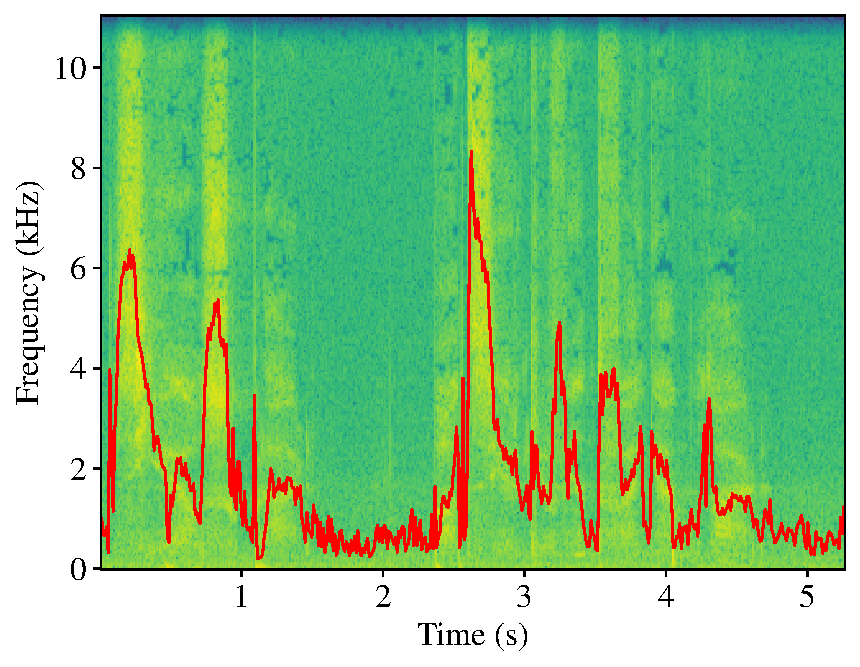
\includegraphics[width = 0.7\textwidth]{chapter6/centreOfGravity.pdf}
    \caption{\centering Spectral centre of gravity for a whispered signal - \\ {\it "Se eu soprar pode ser que o vento venha a mudar"}}
    \label{fig:centreOfGravity}
\end{figure}

\subsection{Feature Mapping}

Also in similar fashion to the work of Perrotin et.al. \cite{perrotinGlottalFlowSynthesis2020}, a sigmoid function was used to map the centre of gravity to a value between 0 and 1, but in this case defining the curve in respect to linear frequency. The sigmoid function is defined as shown in Equation (\ref{eq:cogmapping}), where $F_{vuv}$ and $F_{uv}$ are the two thresholds used to classify the signal as vocalic or unvoiced, and $\lambda$ is the slope of the sigmoid function at the geometric mean of these two frequencies. 

\begin{equation}
    \sigma(f) = \frac{1}{1-\exp\{-(f-\sqrt{F_{vuv}F_{uv}})/\lambda\}}
    \label{eq:cogmapping}
\end{equation}

Figure \ref{fig:sigmoid} shows the sigmoid curve for mapping the centre of gravity to a value between 0 and 1. The curve is defined such that the centre of gravity is mapped to 0 when it is below the unvoiced threshold, and to 1 when it is above the vocalic threshold. The slope of the curve is defined such that the curve is steepest at the geometric mean of the two thresholds, and it is set to 0.5 in this case. The slope of the curve at the average frequency $f_x = \sqrt{F_{vuv}F_{uv}}$ is given by the derivative of the sigmoid function at this point, as shown in the following equations:

\begin{equation}
    \frac{d}{df} \sigma(f) = \frac{\lambda e^{ -\lambda(f-f_x)} }{\left(e^{ -\lambda(f-f_x)} + 1 \right)^2} \text{,}
    \label{eq:sigmoidSlope}
\end{equation}

\begin{equation}
    \frac{d}{df} \sigma(f_x) = \frac{\lambda}{4} \text{.}
\end{equation}

\begin{figure}[H]
    \centering
    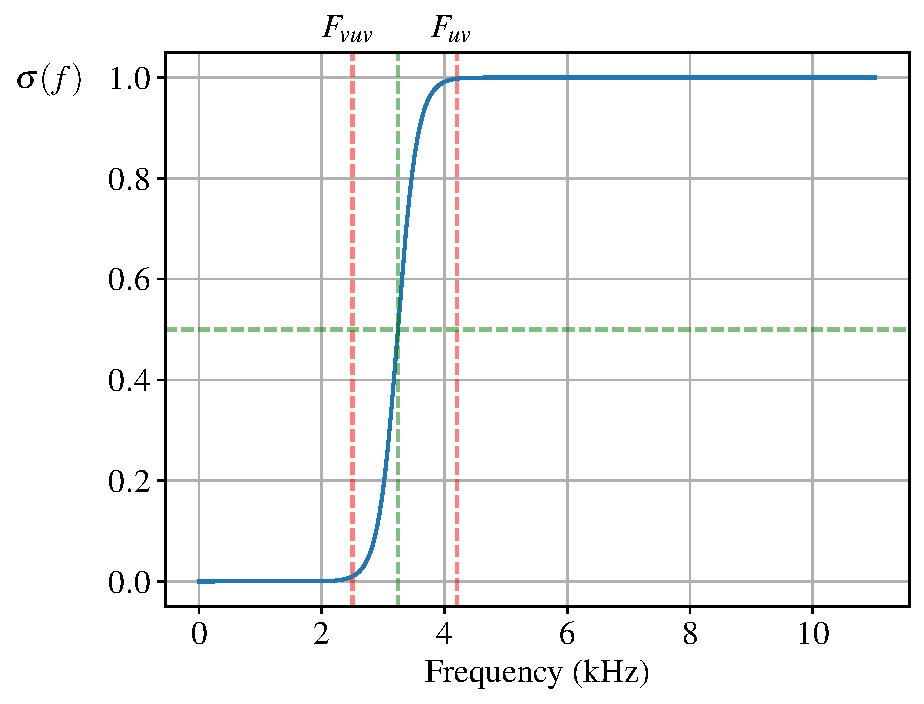
\includegraphics[width = 0.7\textwidth]{chapter6/mapping.pdf}
    \caption{Sigmoid curve for mapping the centre of gravity - $F_{vuv} = 2.5 \text{kHz}$ and $F_{uv} = 4.2 \text{kHz}$}
    \label{fig:sigmoid}
\end{figure}

The slope parameter $\lambda$ can be further parameterized in terms of the two thresholds and a new parameter $\tau$ that defines how much of space between the two points is occupied by the curve, as shown by Equation (\ref{eq:slopeParametrization}) which is adapted from \cite{perrotinGlottalFlowSynthesis2020}.

\begin{equation}
    \lambda = \frac{2}{F_{vuv}- F_{uv}} \log \left (\frac{1+\tau}{1-\tau} \right )
    \label{eq:slopeParametrization}
\end{equation}

Figure \ref{fig:mappedCoG} shows the mapped centre of gravity for the same whispered signal as in \ref{fig:centreOfGravity}, where the signal is classified as fully vocalic when the mapped value is above $F_{vuv}$, and as fully unvoiced when it is below $F_{uv}$. This is used to determine the voicing of the signal, and to trigger the $f_0(t)$ contour to be applied to the voiced segments of the signal.


\begin{figure}[H]
    \centering
    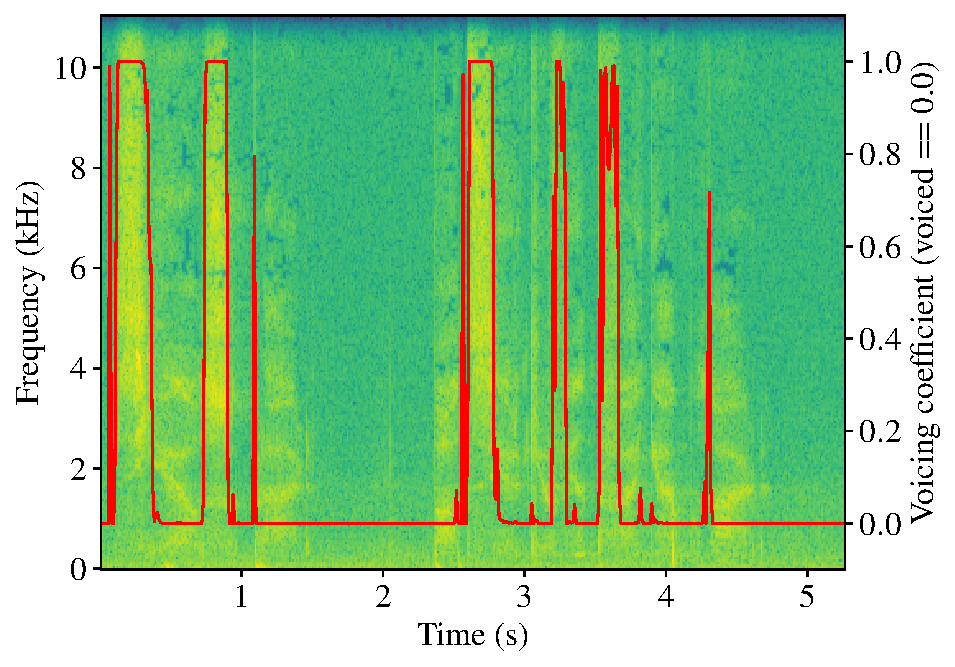
\includegraphics[width=0.7\textwidth]{chapter6/mappedCoG.pdf}
    \caption{\centering Mapped CoG for a whispered signal - {\it "Se eu soprar pode ser que o vento venha a mudar"}}
    \label{fig:mappedCoG}
\end{figure}

In reality, we actually want to always have some noise in the source excitation signal in order to avoid the presence of a purely voiced component as this can still sound unnatural. As such, in the actual system the mapping curve is scaled and shifted by a small constant factor to ensure that some level of noise is added even in purely voiced/vocalic segments. This value has been determined empirically in order to maximize the perceived naturalness of the synthesized speech.

\section{Implementation}

The first implementation of the overlap add reconstruction of voiced speech is presented in listing \ref{lst:pythonConversion}, where the system is implemented in Python for the sake of validation, as was done in the previous chapters. The results that were extracted for perceptual testing and evaluation were taken from the Python implementation, as proven in Chapters \ref{chap:pulseGen} and \ref{chap:filt}, this model has lower noise levels than the realtime physical system, and better representation of microfrequency changes to the fundamental frequency.

The system processes the input whispered speech in overlapping frames of 512 samples each. This overlap ensures continuity and smooth transitions between frames. Each input frame is windowed using the Hanning sine window, as shown in Equation (\ref{eq:windowFunc}), to reduce spectral leakage. The concatenated input frames are then subjected to the ODFT to obtain the PSD of the current frame.  In parallel, the system determines whether each frame contains voiced or unvoiced speech using the spectral centre of gravity presented previously, which gets mapped through a sigmoid function. The WAD algorithm further refines this classification by considering the energy and zero-crossing rate of the frame, ensuring that only segments with actual speech activity are processed for voicing.

Once the voiced/unvoiced decision is made, the system generates excitation signals accordingly, based on the method proposed in Figure \ref{fig:pulseGenFlow}. For voiced segments, a glottal pulse is synthesized based on the $F_0$ contour. For unvoiced segments, white noise of the same length is generated.  These excitation signals are then filtered using an LPC filter designed from the interpolated PSD of the current and previous frames. In fact, for the results presented in the next chapter, both individual pulse filtering and frame-wise filtering were used, in order to compare the impact that the smoother filter transitions have on the naturalness of the final output. %The filtered excitation signals are then added to the output buffer directly in the time domain, overlapping over top of each other. This method ensures that each frame contributes smoothly to the final output signal, maintaining continuity and naturalness. The reconstructed speech is normalized to the 16-bit PCM range to match the typical audio format used in digital systems. This step-by-step approach, combining spectral analysis, excitation generation, and LPC filtering, effectively transforms whispered speech into a more intelligible and natural-sounding voiced speech signal.

Figure \ref{fig:frameFilteringWaveform} shows the results of the individual pulse filtering and frame-wise filtering mechanisms for a given frame of whispered speech. It is to be noted that the pulse-by-pulse filtering results in a visually smoother waveform, which can be beneficial for the naturalness of the final output. The results of the perceptual testing and evaluation of the system are presented in the next chapter.

\begin{figure}[H]
    \centering
    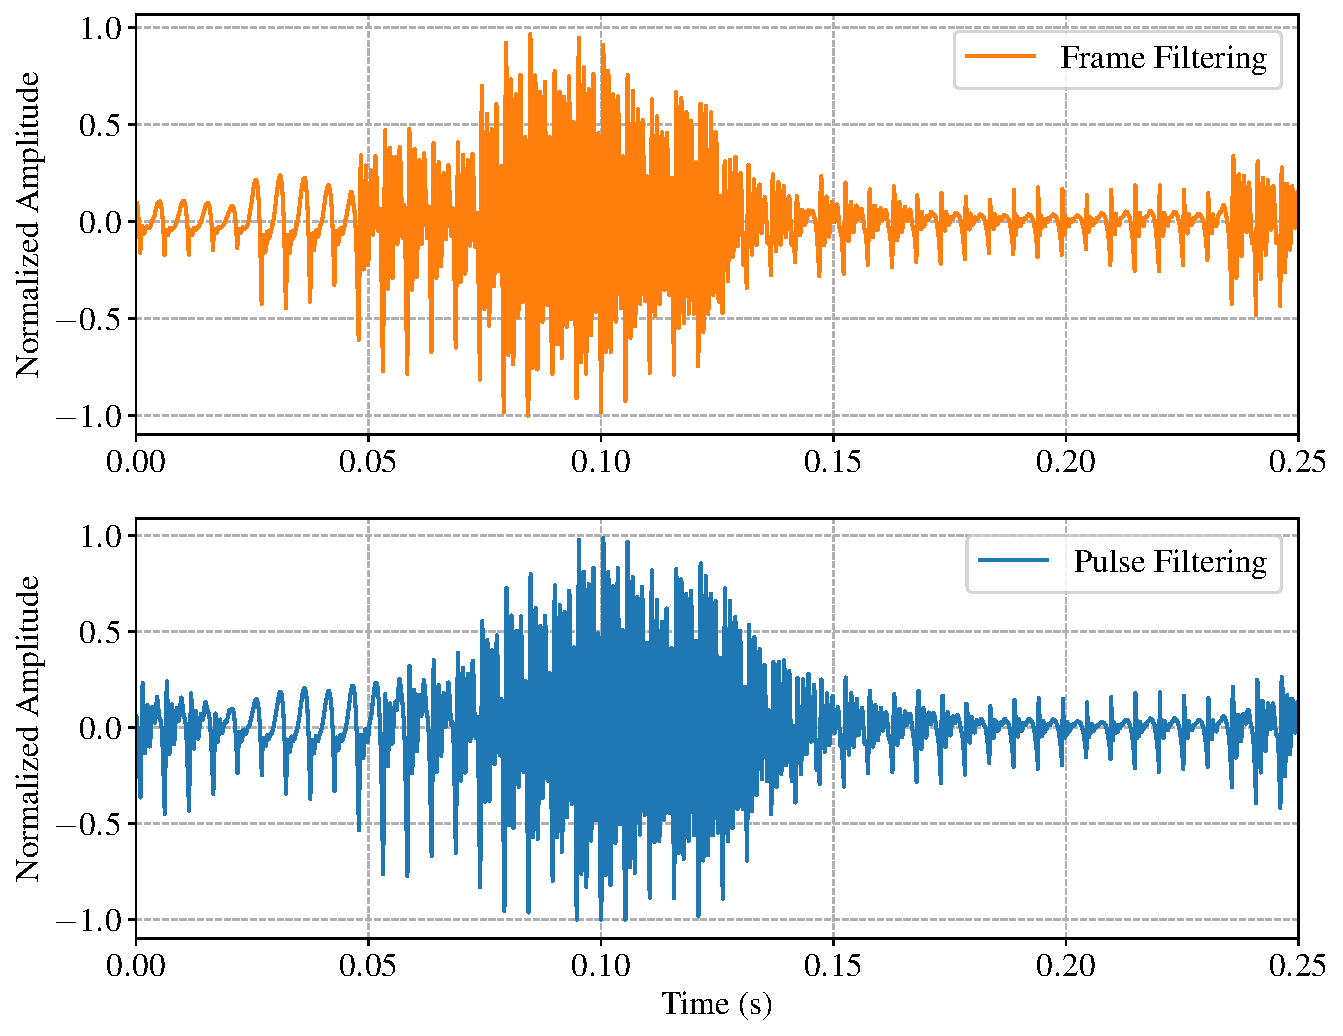
\includegraphics[width = 0.9\textwidth]{chapter6/electrolarynx.pdf}
    \caption{Frame filtered (above) and individually filtered (below) pulses}
    \label{fig:frameFilteringWaveform}
\end{figure}

Meanwhile, Figure \ref{fig:segmentedWaveform} shows the results of the whispered speech segmentation algorithm, where the unsegmented whispered speech is shown above, and the segmented whispered speech is shown below. It is to be noted that the segmentation algorithm is able to detect the voiced and unvoiced segments of the signal, which is crucial for the proper application of the $F_0$ contour and the generation of the excitation signals. The figure makes it clear that the unvoiced segments when identified are then excited by noise, and the voiced segments are excited by the glottal pulses generated by the $F_0$ contour, mixed with a lower level of noise.

\begin{figure}[H]
    \centering
    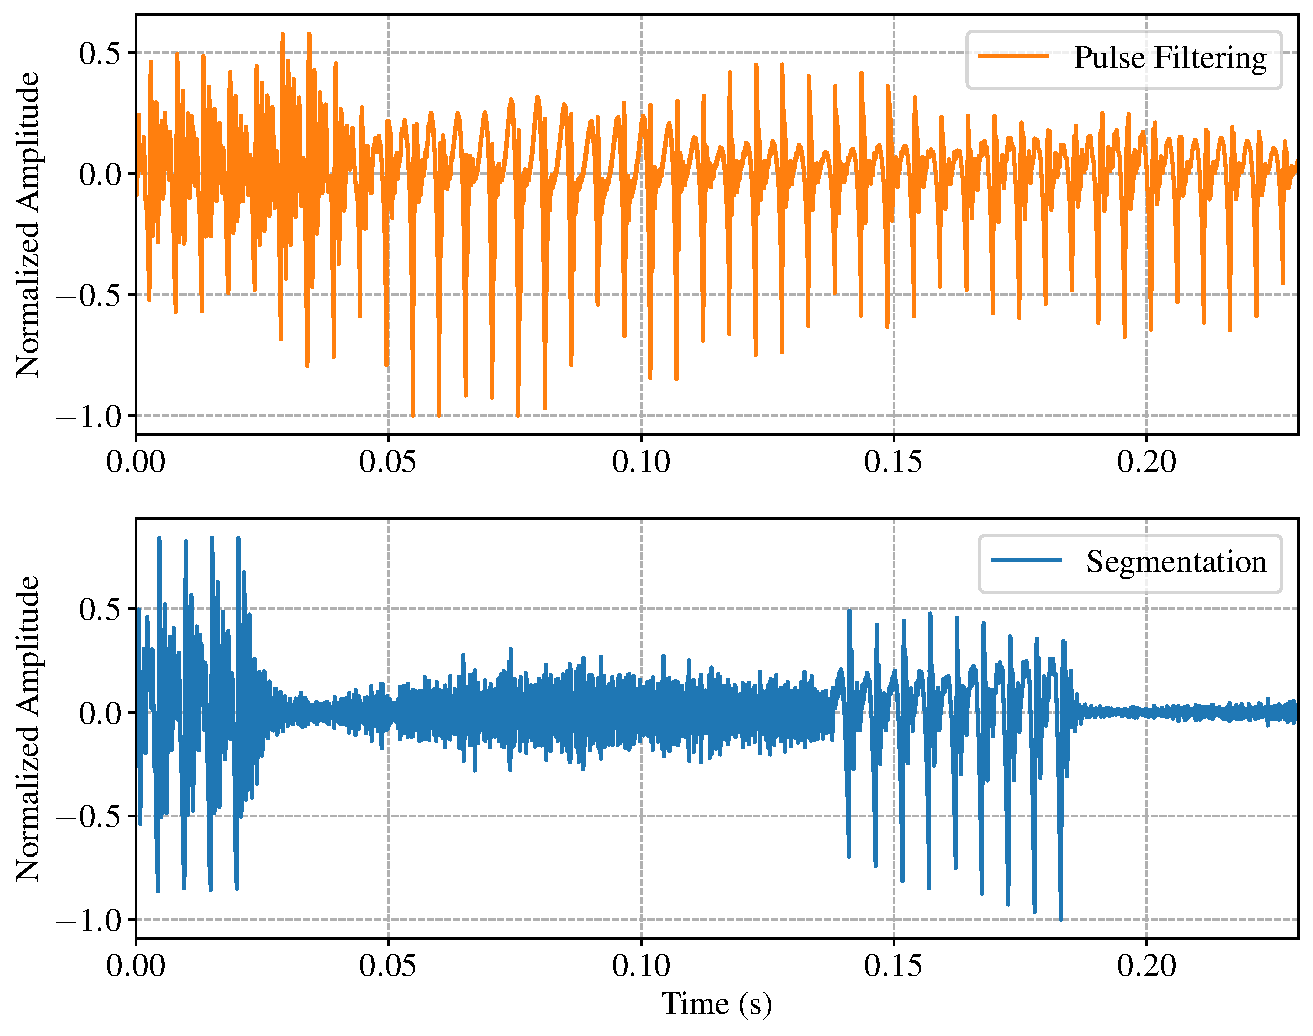
\includegraphics[width = 0.9\textwidth]{chapter6/segmentation.pdf}
    \caption{Unsegmented (above) and segmented (below) whispered speech}
    \label{fig:segmentedWaveform}
\end{figure}

%\vspace*{12mm}

\subsection{Realtime Implementation}

The system was also implemented in the STM32 environment for realtime operation. As we're using the same LPC filter as in chapter \ref{chap:filt}, the system works in the same way, with the only differences being that for each pulse the PSD is interpolated between the current and previous frames, and that the pulse is filtered in the time domain by the LPC filter. Listing \ref{lst:segmentationC} shows the implementation of the conversion algorithm in C, that was developed on top of the main function shown in listing \ref{lst:pythonConversion}.

Another relevant aspect that is worth mentioning is that of the noise signal generation. Where as in python the noise signal was generated using a normal distribution, in the STM32 environment the noise signal is generated using a simpler pseudo-random number generator. The STM32F746ng does feature the RNG peripheral, but it was decided that the use of this peripheral would be overkill for the purposes of this project, and that a much simpler Linear Congruential Generator (LCG) \cite{Iserles_1989} would suffice. The generator is implemented as shown in listing \ref{lst:noiseGenC}, and it is used to generate the noise signal that is used to excite the unvoiced segments of the signal.

\begin{lstlisting}[language=C, caption={LCG implementation in C}, label={lst:noiseGenC}]
static uint32_t seed = 1337;
#define LCG_A 1664525       // LCG multiplier
#define LCG_C 1013904223    // LCG increment
#define LCG_M 0xFFFFFFFF    // LCG modulus 2^32 - 1

/// @brief Generate a pseudo-random integer using a Linear Congruential Generator
/// @return Random integer
uint32_t randInt(){
    seed = (LCG_A * seed + LCG_C) % LCG_M;
    return seed;
}

/// @brief Generate a pseudo-random float
/// @return Random 32bit float
float32_t randFloat(){
    return 2.0f * ((float32_t) randInt() / (float32_t) LCG_M) - 1.0f;
}
\end{lstlisting}

The computation of the centre of gravity and it's mapping are also done in the STM32 environment, essentially in the same fashion as in the Python validation. As the operation is effectively a simple weighted average of the power spectrum, and the code is shown in listing \ref{lst:cogC}.

\begin{lstlisting}[language=C, caption={Centre of Gravity computation in C}, label={lst:cogC}]
/// @brief Compute the spectral centre of gravity from a frame's PSD
/// @param psd Power Spectral Density
/// @param n Total number of samples (1024)
/// @param fs Sampling Frequency
/// @return Spectral Centre of Gravity
float32_t centreOfGravity(float32_t* psd, int n, float32_t fs){
    float32_t num = 0, dem = 0;

    for (size_t i = 0; i < n / 2; i++){
        dem += psd[i];
        num += (i * fs / n) * psd[i];
    }

    return num / dem;
}

/// @brief Mapping sigmoid for computing the centre of gravity
/// @param cog Centre of gravity frequency
/// @param Fvuv Vocalic whispered threshold
/// @param Fuv Unvoiced frequency threshold
/// @param tau Sharpness coefficient (0.99)
/// @return mapped mixing coefficient
float32_t mapping(float32_t cog, float32_t Fvuv, float32_t Fuv, float32_t tau){
    float32_t k = (cog - sqrtf(Fvuv*Fuv)) * 2/(Fuv - Fvuv) * log10((1+tau)/(1-tau));    
    
    return 1/(1 + exp(-k));
}
\end{lstlisting}

One component of the system that wasn't included in the STM32 implementation shown in listing \ref{lst:segmentationC} was the whisper activity detection algorithm from previous subsections. This is due to the high computational demand of determining the zero crossing rate and energy of the signal for each frame, which made the audio produced by the STM32 stutter and fail to run in realtime. As such, the system was run in a continuous voiced mode, without the $F_0$ contour that had been established previously, which lead to some loss in perceived prosody. Despite this, the code for the whisper activity detection method is shown in listing \ref{lst:wadC}.

Due to time constraints and the effect that the board noise has on the quality of the conversion algorithm output, the results shown in the following section were taken from the Python implementation. The STM32 implementation was used to validate the conversion algorithm and to ensure that the system could run in real-time, but the results were not used for the perceptual testing and evaluation.
\chapter{System configuration and assessment} \label{chap:results}

With the complete system running, it is now possible to discuss the results of the proposed system. In this chapter, we will discuss not only the results obtained, but also the preprocessing steps that were taken in order to obtain them, and the testing methodology that was used in order to conduct the perceptual tests. The results will be discussed in the context of the proposed system architecture, and the whisper activity detection and speech segmentation algorithms that were used in the proposed system for silence detection and Voiced/Unvoiced decisions.

\section{Dataset and Preprocessing}

For the data, the original DyNaVoiceR dataset \cite{JESUS2023101223} was utilized, which is a matched dataset of both voiced and whispered speech utterances that were recorded within a controlled environment in a soundproof room and high quality recording equipment \cite{castilho2019fct}. The database consisted of 13 sustained sounds, i.e. vowels and sibilants from european portuguese, 28 words, 6 short phrases and a small text. These were uttered by 30 speakers, with an equal representation of male and female genders. From this, a smaller subset of just 4 samples of two phrases from different speakers was done, in order to test the proposed system.

\begin{table}[H]
    \centering
    \begin{tabular}{cc}
        \hline
        Test Phrase & Speaker \\
        \hline \hline
        \multirow{2}*{\textit{A asa do avião andava avariada}} & SPF05 \\
        & SPM18 \\
        \hline
        \multirow{2}*{\textit{O tiago comeu quatro pêras}} & SPF12 \\
        & SPM14 \\
        \hline
    \end{tabular}
    \caption{Samples user for testing}
    \label{tab:dataset}
\end{table}

\subsection{Fundamental Frequency Analysis}

In order to maximize the quality of the comparisons between converted whispered speech and the reference samples, the fundamental frequency of the reference samples was analyzed in order to obtain the average fundamental frequency of each sample. This was achieved by means of the probabilist Yin algorithm \cite{mauchPYINFundamentalFrequency2014}, which is a robust and efficient algorithm for monophonic fundamental frequency estimation. Librosa provides this algorithm as a function \texttt{pyin()} \cite{mcfee_2024_11192913}, which was used to analyze the fundamental frequency of the reference samples, the results of which are shown in Figure \ref{fig:f0analysis}.

\begin{figure}[H]
    \centering
    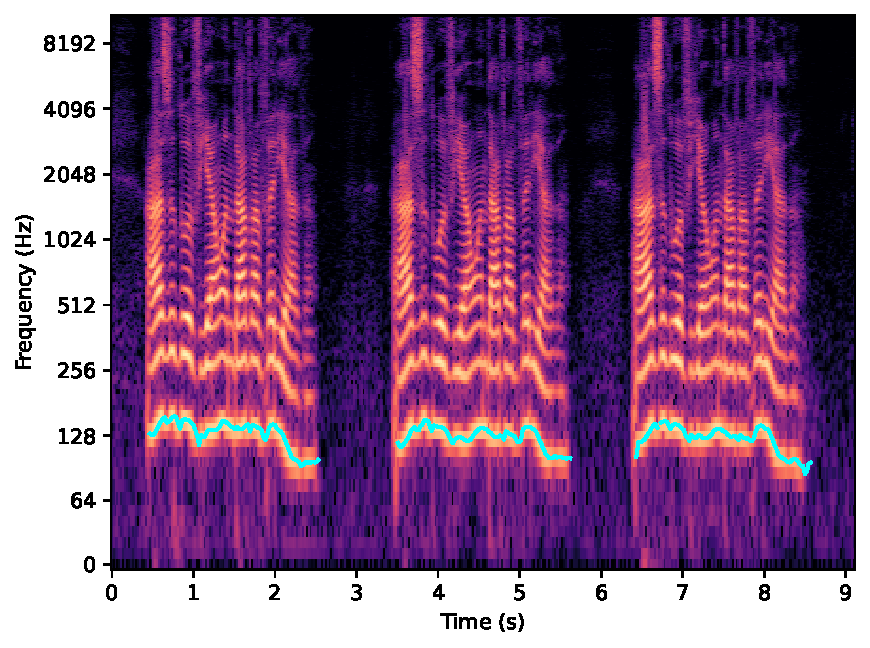
\includegraphics[width=0.75\textwidth]{chapter7/f0analysis.pdf}
    \caption{Fundamental frequency analysis of a voiced reference sample - Subject SPM18}
    \label{fig:f0analysis}
\end{figure}

\subsection{Noise Removal and Audio Restoration}

Due to the nature of the dataset and the recording methodology chosen, the whispered speech was recorded with a much higher gain than the voiced speech, which made it necessary to preprocess all whispered samples in order to remove background noise. Also, due to the higher gain, the whispered samples had much more clicking and slight popping sounds, due to lips and tongue smacking, which also had to be removed. For this, Adobe Audition 2024 was used to attenuate both of these.

First the noise was removed using the noise reduction effect, by first selecting a portion of the audio that was just noise (i.e. no whispered speech nor breathing) and then applying the noise reduction effect with the automatic settings. These proved to be quite effective at removing most of the noise that interfered with the whispered speech detection and segmentation algorithms. After this, the clicking sounds were removed with the Click/Pop Eliminator process \cite{adobe_audition_noise_reduction}, with the settings set empirically on a sample-by-sample basis, in order to remove the clicking sounds without affecting the whispered speech.

Besides this, the audio was normalized to not exceed -12dB, in order to avoid clipping and to ensure that the converted audio samples would remain in the same loudness range in relation to the reference and each other. For this, Ableton Live 11 was used, with a limiter applied to all audio samples with a gain of +6dB and a ceiling of -12dB, using automatic lookahead and release settings. 

\section{Testing Environment}

In order to gather the perceptual data for the proposed system, a MUSHRA listening test was conducted with responses from 17 volunteers, with ages ranging from 22 to 61. Multiple Stimuli with Hidden Reference and Anchor (MUSHRA) \cite{internationaltelecommunicationunionBS15343Method2015} is a testing methodology that is widely used in audio and speech quality assessment, where listeners are asked to rate and compare the quality of different audio samples. It works by presenting the listener with a set of audio samples, where one of them is a reference sample, and the listener is asked to rate the quality of other samples in relation to the reference.

Considering this, a testing environment was deployed using the open source platform webMUSHRA platform \cite{schoefflerWebMUSHRAComprehensiveFramework2018}. This was in turn deployed using PyMushra which is yet another open-source project that is meant to simplify the deployment of the webMUSHRA framework, by providing a simple Flask web server and a tinydb database for the storage of the results. This last python package also supports exporting the data results directly to a python environment as a Pandas dataframe, allowing for quick statistical analysis using SciPy and visualization using Seaborn.


\subsection{Whispered-to-Speech Conversion}

As mentioned in the previous chapter, the tests that are conducted in terms of whispered to speech conversion are first implemented using individual pulse filtering as per the scheme in Figure \ref{fig:pulseMap} and another one by computing one filter per frame, so as to obtain an idea of the improvement that the filter interpolation mechanism brings to the system. In comparison, we will have the complete system using the activity detection, speech segmentation and $F_0$ contour, in order to evaluate the improvement in prosody and overall quality that these mechanisms contribute in terms of conversion. The parameters that were used for the whispered-to-speech conversion are shown in table \ref{tab:w2cSettings}.


\begin{table}[H]
    \centering
    \begin{tabular}{cccc}
        \hline
        Speaker & $F_{vuv}$ (Hz) & $F_{uv}$ (Hz) & Avg. $F_0$ (Hz)\\
        \hline \hline
        SPF05 & 2400 & 3400 & 191.65 \\ \hline 
        SPF12 & 2400 & 3400 & 165.33 \\ \hline
        SPM14 & 1800 & 2400 & 111.30 \\ \hline
        SPM18 & 1800 & 2400 & 127.60 \\ \hline
    \end{tabular}
    \caption{\centering Centre of gravity thresholds and average fundamental frequency \\ for each of the converted samples}
    \label{tab:w2cSettings}
\end{table}

The testing page is shown in Figure \ref{fig:mushraW2C}, where the user is presented with the reference sample, the converted sample and a feedback form. Here, the test subject is presented with the reference voiced audio and 5 randomized stimuli samples. These are: the hidden reference, the original whispered audio, the full system conversion and the two intermediary steps of individual pulse filtering and frame-by-frame filtering. The latter is presented as representation of the EL, which is compared with the individual pulse filtering and the segmented conversion. Table \ref{tab:w2cConditions} provides a brief description of the test conditions that were used for the whispered-to-speech conversion tests.

\begin{table}[H]
    \centering
    \begin{tabular}{p{0.2\textwidth}p{0.6\textwidth}}
        \hline 
        Test Condition & Description \\
        \hline \hline
        Reference & Voiced reference sample \\
        Whispered & Original whispered sample \\
        Frame Filtering & WSC using a single filter for each audio segment \\
        Pulse Filtering & WSC using filtering for each individual glottal pulse\\
        Complete System & WSC using pulse filtering, along with the $F_0$ contour, silence detection using WAD and segmentation with V/UV decisions \\
        \hline
    \end{tabular}
    \caption{Whispered-to-Speech conversion test conditions}
    \label{tab:w2cConditions}
\end{table}
    
The user is then asked to rate the samples in terms of how intelligible and natural it sounds, and how good the audio samples are in terms of overall quality. A scale is provided where the scores are labeled in the following manner: 0-20 is bad, 20-40 poor, 40-60 fair, 60-80 good and 80-100 is excellent.

\subsection{Vowel synthesis}

Another test was conducted in order to evaluate how natural the pulse generation and the filtering mechanisms presented in Chapters \ref{chap:pulseGen} and \ref{chap:filt}, respectively, are in terms of vowel synthesis. Here the reference is the original voiced vowel, and the stimuli are the completely synthesized vowels along with the reference. In the former case, two types of vowels are generated, one with a constant $F_0$ frequency and the other following the $F_0$ contour that was established in Chapter \ref{chap:pulseGen}.

All five vowels were then concatenated into a single audio file for each stimuli, and the user was asked to rate the samples in the same manner as the whispered-to-speech conversion test. The testing page is shown in Figure \ref{fig:mushraVowel}.  

\section{Results and Discussion}

The results of all tests are presented in the following subsections. For all tests, all recorded data points were used, and the results were analyzed using the mean, variance and the bilateral 95\% confidence interval. Also paired t-tests were conducted in order to determine if the differences between the results were statistically significant, with a significance level (p-value) of 0.05.

\subsection{Whispered-to-Speech Conversion}

Figures \ref{fig:w2sTiago} and \ref{fig:w2sAviao} show the results of the whispered-to-speech conversion tests for the phrases \textit{"O Tiago comeu quatro pêras"} and \textit{"A asa do avião andava avariada"}, respectively, presented in a box and whisker plot indicating the distribution of each quartile of data. All data points are also shown in the plot as the gray dots, along with white circles that indicate outliers. The other results from statistical analysis are presented in Table \ref{tab:w2s}.

\begin{figure}[H]
    \centering
    \begin{minipage}[H]{0.495\textwidth}
        \centering
        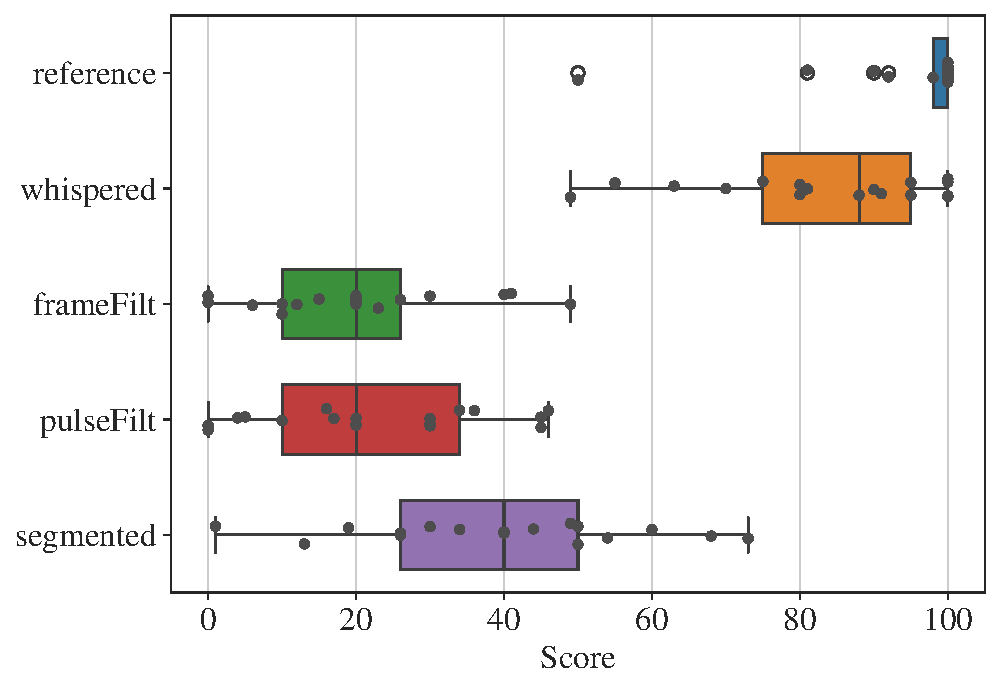
\includegraphics[width=\textwidth]{chapter7/SPF05_aviao.pdf}
        \subcaption{SPF05}
    \end{minipage}
    \begin{minipage}[H]{0.495\textwidth}
        \centering
        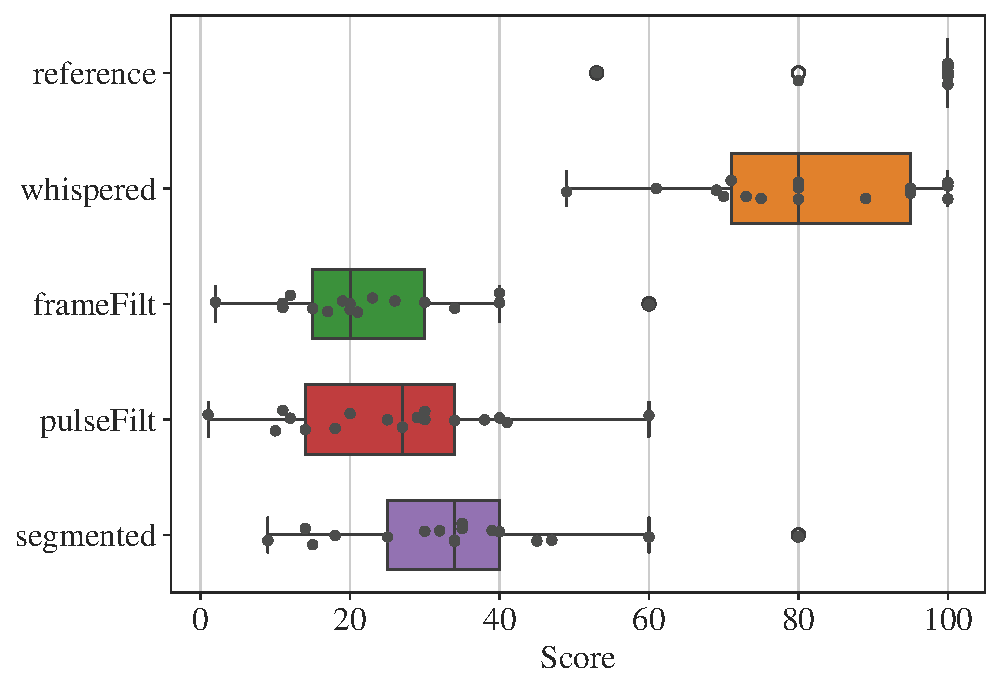
\includegraphics[width=\textwidth]{chapter7/SPM14_tiago.pdf}
        \subcaption{SPM14}
    \end{minipage}
    
    \caption{\centering Whispered-to-Speech conversion results - \\ \textit{"O Tiago comeu quatro pêras"}}
    \label{fig:w2sTiago}
\end{figure}

\begin{figure}[H]
    \centering
    \begin{minipage}[H]{0.495\textwidth}
        \centering
        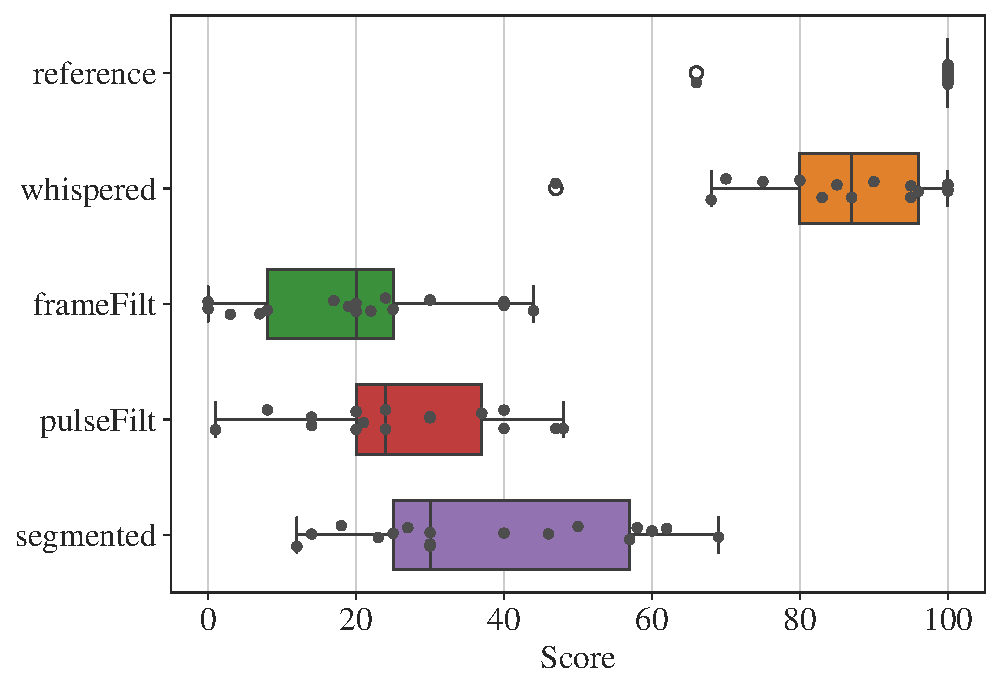
\includegraphics[width=\textwidth]{chapter7/SPF12_tiago.pdf}
        \subcaption{SPF12}
    \end{minipage}
    \begin{minipage}[H]{0.495\textwidth}
        \centering
        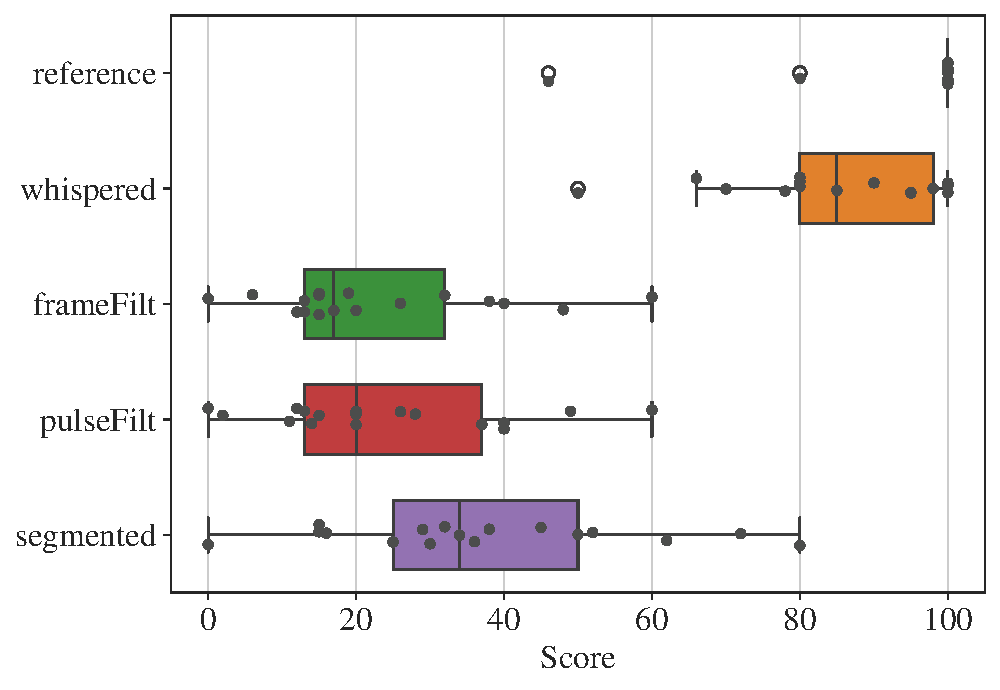
\includegraphics[width=\textwidth]{chapter7/SPM18_aviao.pdf}
        \subcaption{SPM18}
    \end{minipage}
    \caption{\centering Whispered-to-Speech conversion results - \\ \textit{"A asa do avião andava avariada"}}
    \label{fig:w2sAviao}
\end{figure}

The results show that the complete system is able to outperform the individual pulse filtering and frame filtering mechanisms, with higher mean scores than both. This does show that the proposed system is able to generate more natural sounding speech that these other two steps, which is in line with the expectations. Both the frame filtering and individual pulse filtering represent naturalness and intelligibility levels akin to that of a EL device, showing that the effect of both segmentation and $F_0$ contour has quite a significant impact in the conversion process.

By doing a paired t-test, as shown in Tables \ref{tab:pairwiseSPF05}, \ref{tab:pairwiseSPF12}, \ref{tab:pairwiseSPM14} and \ref{tab:pairwiseSPM18}, it was found that the differences were statistically significant for all samples, except for the comparison between the individual pulse filtering and the frame filtering where p > 0.05, indicating that the differences between these two are not statistically significant. Despite this, the means between these two are slightly different, with the pulse-wise filtering having a slightly higher mean than the frame-wise mechanism, which is in line with the expectations.

The main reason for this is that the hard filter changes that are done by computing a filter per frame, are not as smooth and introduce a spring reverb-like periodic artifact that is noticeable after long periods of listening. This is not present in the individual pulse filtering mechanism, which is able to generate a smoother and more natural sounding speech, as the filter is computed for each pulse and then interpolated between them.

\begin{table}[H]
    \centering
    \begin{tabular}{crcccc}
        \hline
         & & SPF05 & SPF12 & SPM14 & SPM18 \\ \hline

        \multicolumn{1}{l|}{\multirow{3}*{Reference}} & $\mu$ & 94.765 & 98.000 & 96.059 & 95.647 \\ %\cline{2-6}
        \multicolumn{1}{l|}{} & $\sigma^2$ & 12.657 & 8.246 & 12.106 & 13.679 \\ 
        \multicolumn{1}{l|}{} & $CI_{95\%}$ & $\pm$ 6.02 & $\pm$ 3.92 & $\pm$ 5.75 & $\pm$ 6.50\\ \hline

        \multicolumn{1}{l|}{\multirow{3}*{Whispered}} & $\mu$ & 83.059 & 85.353 & 81.588 & 85.118 \\ %\cline{2-6}
        \multicolumn{1}{l|}{} & $\sigma^2$ & 16.157 & 14.491 & 15.383 & 14.260 \\ 
        \multicolumn{1}{l|}{} & $CI_{95\%}$ & $\pm$ 7.68 & $\pm$ 6.89 & $\pm$ 7.31 & $\pm$ 6.78 \\ \hline

        \multicolumn{1}{l|}{\multirow{3}*{Complete System}} & $\mu$ & 39.824 & 38.294 & 34.823 & 37.118 \\ %\cline{2-6}
        \multicolumn{1}{l|}{} & $\sigma^2$ & 19.340 & 18.289 & 17.458 & 21.254 \\ 
        \multicolumn{1}{l|}{} & $CI_{95\%}$ & $\pm$ 9.19 & $\pm$ 8.69 & $\pm$ 8.30 & $\pm$ 10.10 \\ \hline

        \multicolumn{1}{l|}{\multirow{3}*{Pulse Filtering}} & $\mu$ & 22.824 & 25.765 & 25.882 & 23.941 \\ %\cline{2-6}
        \multicolumn{1}{l|}{} & $\sigma^2$ & 15.709 & 13.339 & 14.521 & 16.479 \\ 
        \multicolumn{1}{l|}{} & $CI_{95\%}$ & $\pm$ 7.45 & $\pm$ 6.34 & $\pm$ 6.63 & $\pm$ 7.51 \\ \hline

        \multicolumn{1}{l|}{\multirow{3}*{Frame Filtering}} & $\mu$ & 20.118 & 19.941 & 23.588 & 22.882 \\ %\cline{2-6}
        \multicolumn{1}{l|}{} & $\sigma^2$ & 13.946 & 13.539 & 13.938 & 15.791 \\ 
        \multicolumn{1}{l|}{} & $CI_{95\%}$ & $\pm$ 6.63 & $\pm$ 6.44 & $\pm$ 6.90 & $\pm$ 7.83 \\ \hline
    
    \end{tabular}
    \caption{Whispered-to-Speech conversion results}
    \label{tab:w2s}
\end{table}

Overall, the results show that the proposed system is able to generate more natural sounding speech than the individual pulse filtering and frame filtering mechanisms, with the complete system having a higher mean score than both. This is in line with the expectations, as the proposed system is able to generate a more natural sounding speech by interpolating the filters between pulses and by using the $F_0$ contour to generate a more natural prosody. Most users did although report that the whispered speech was still quite intelligible, which could be due to the gain of it being higher in the original dataset recording, which could have made it easier to understand. Perhaps, lowering the gain of the whispered speech to a more realistic level (such that idle noise levels were comparable to that of the voiced speech samples) could have made the whispered speech more difficult to understand, and thus the conversion more effective.

\mybreak

\subsection{Vowel Synthesis}

The results for the vowel synthesis test are presented in Figure \ref{fig:vowels} in the same style of box and whispers plot as the previous test. These are shown alongside with the mean, standard variance and the 95\% confidence interval in Table \ref{tab:vowelSynth}. 

%Next the results of the vowel synthesis test are presented in figure \ref{fig:vowels} and table \ref{tab:vowelSynth}. The results show that the complete system is able to generate more natural sounding vowels than the individual pulse filtering mechanism, with the mean score being higher for the complete system than the individual pulse filtering mechanism. This is in line with the expectations, as the proposed system is able to generate a more natural sounding speech by interpolating the filters between pulses and by using the $F_0$ contour to generate a more natural prosody. The differences between the two are statistically significant, with p < 0.05, indicating that the differences between the two are statistically significant.

\begin{figure}[H]
    \centering
    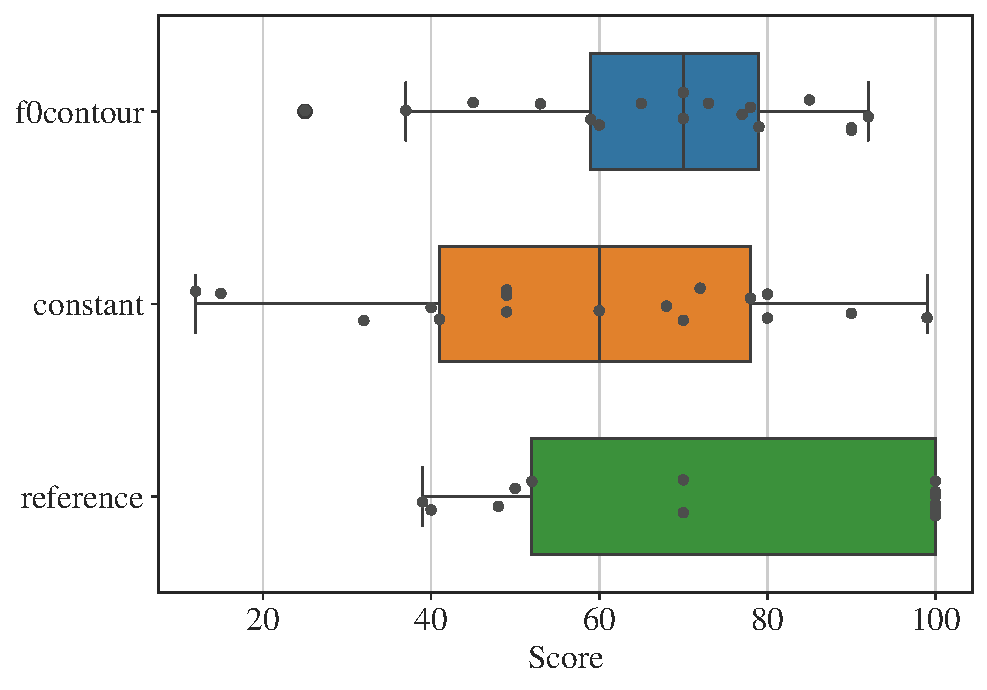
\includegraphics[width = 0.5\textwidth]{chapter7/vowels.pdf}
    \caption{Vowel synthesis results}
    \label{fig:vowels}
\end{figure}

\begin{table}[H]
    \centering
    \begin{tabular}{lccc}
        \hline
        & Reference & Constant $F_0$ & Contour $F_0$ \\
        \hline

        $\mu$ & 80.529 & 57.882 & 67.529 \\ %\cline{2-6}
        $\sigma^2$ & 25.229 & 25.017 & 19.174 \\
        $CI_{95\%}$ & $\pm$ 11.99 & $\pm$ 11.89 & $\pm$ 9.11 \\ \hline
    
    \end{tabular}
    \caption{Vowel synthesis results}
    \label{tab:vowelSynth}
\end{table}

From this, it is clear that the synthesized vowels generated with the $F_0$ contour generally performed with a higher mean score than the constant $F_0$ frequency, which is in line with the expectations. This is due to the fact that the $F_0$ contour being defined to simulate some sort of natural sounding prosody, which is able to generate a more natural sounding speech. From the pairwise t-test results shown in table \ref{tab:pairwiseVowel}, it is clear that the differences between the synthesized vowels are statistically significant, with p < 0.05. Despite this, all the stimuli have shown higher variance indicating that the quality of the synthesized vowels and the reference is not as consistent as the whispered-to-speech conversion tests.

\begin{table}[H]
    \centering
    \begin{tabular}{lcccc}
        \hline
        & Reference & Constant $F_0$ & Contour $F_0$ \\
        \hline
        Reference & - & 4.70e-02 & 4.95e-11 \\
        Constant $F_0$ & 4.70e-02 & - & 6.99e-11 \\
        Contour $F_0$ & 4.95e-11 & 6.99e-11 & - \\
        \hline
    \end{tabular}
    \caption{Pairwise P-Values for Vowel Synthesis}
    \label{tab:pairwiseVowel}
\end{table}


%\vspace*{12mm}

\chapter{Conclusion} \label{chap:conclusion}

This thesis has presented a novel approach to whispered-to-voiced speech conversion using synthetic voicing techniques. The conclusions drawn from this research can be attributed to the performance of the proposed platform and the perceptual data that has been collected. The following sections summarize the contributions, limitations, and future work, along with the final remarks and acknowledgements.

First of all, the proposed system has demonstrated the feasibility of the conversion in a realtime scenario, with the ability to generate voiced speech from whispered input on-the-fly without any significant delays. The system architecture, comprising the glottal pulse generation and vocal tract filter modelling modules, has been successfully implemented and integrated into the STM32 platform. Despite the limited computational resources of the development platform, especially regarding the pulse generation, promising results have been obtained in terms of speech quality and intelligibility.

Moreover, the whispered speech detection and segmentation algorithms have proven to be effective in identifying the voiced and unvoiced regions of the input signal, allowing for the selective application of synthetic voicing, using a lightweight and efficient criteria. Despite this, this criteria is applied on a frame-by-frame basis, which may lead to discontinuities in the generated speech, especially in the presence of noise or rapid changes in the input signal from phoneme to phoneme.

Future work should focus on improving the voiced speech generation by perhaps exploring other realtime processing platforms such as PortAudio, which could provide more computational resources and allow for more sophisticated algorithms to be implemented. The integration of a more robust whispered speech detection and segmentation algorithm, capable of identifying phoneme boundaries and transitions, could also improve the quality of the generated speech. Machine learning techniques could also be employed to enhance the system's performance by providing more accurate estimates of voicing decisions and the fundamental frequency that is to be applied to the synthetic pulses. Perhaps the existing segmentation models could be improved upon by pretraining and learning the parameters for centre of gravity mapping and the WAD algorithm. This could be achieved by using the existing labeled data, which includes markings for voiced and unvoiced regions, to train a machine learning model that can predict the optimal parameters for the segmentation algorithms. This could potentially improve the accuracy of the segmentation and reduce the discontinuities in the generated speech. 

%\vspace*{12mm}

%% comment next 2 commands if numbered appendices are not used
\appendix
\chapter{Code Snippets} \label{ap1:loren}
 
\section{Pulse Generation}

\begin{lstlisting}[language=C, caption={Buffer processing function.}, label={lst:processBuffer}]
    void process_buffer(float32_t *mainBuf) {
        int16_t *rx_buf, *tx_buf;
    
        if (rx_buffer_proc == PING)
            rx_buf = (int16_t *)PING_IN;
        else
            rx_buf = (int16_t *)PONG_IN;
    
        if (tx_buffer_proc == PING)
            tx_buf = (int16_t *)PING_OUT;
        else
            tx_buf = (int16_t *)PONG_OUT;
    
        int16_t sampleL, sampleR;
        for (int i = 0; i < (PING_PONG_BUFFER_SIZE); i++){
            // read both input samples
            sampleL = *(rx_buf++); sampleR = *(rx_buf++);
    
            // copy the input buffer to the output buffer
            *(tx_buf++) = (int16_t) floor((float32_t) 0.5 + mainBuf[i]);
            *(tx_buf++) = sampleR; // RIGHT channel remains untouched
        }
    
        RX_buffer_full = 0;
        TX_buffer_empty = 0;
    }
\end{lstlisting}

\begin{lstlisting}[language=C, caption={Pulse generation \texttt{main()} funciton.}, label={lst:mainPulseGen}]
int main(void) {
    uint16_t idxMainBuf = 0, vibrato = 0, contourIndex = 0; // reset main buffer index
    uint16_t gPulseLen, lastPulseLen, filteredLength;

    float32_t mainBuf[2 * PING_PONG_BUFFER_SIZE] = {0.0f};
    float32_t gPulseBuf[MAX_PULSE_BUFFER] = {0.0f}; // 220 ~ 22050/100

    stm32f7_wm8994_init(AUDIO_FREQUENCY_22K, // 22050 Hz
                        IO_METHOD_DMA,
                        INPUT_DEVICE_INPUT_LINE_1,
                        OUTPUT_DEVICE_HEADPHONE,
                        WM8994_HP_OUT_ANALOG_GAIN_0DB,
                        WM8994_LINE_IN_GAIN_0DB,
                        WM8994_DMIC_GAIN_9DB,
                        SOURCE_FILE_NAME,
                        NOGRAPH);

    // generate single prototype pulse 10% shorter than that of the fundamental period
    gPulseLen = genPulse(FS, F0 * 1.1, gPulseBuf, PULSE_GAIN);

    for(;;){
        while (!(RX_buffer_full && TX_buffer_empty)){}

        // 1. Copy first half to the output during the DMA processing
        process_buffer(mainBuf); 

        // 2. Copy second half to first half
        for (size_t i = 0; i < N; i++){
            mainBuf[i] = mainBuf[i + N];
            mainBuf[i + N] = 0.0f;
        }

        // Place pulses inside the buffer
        while (idxMainBuf < N){
            lastPulseLen = getPulseLen(FS, contour[contourIndex]);

            // add vibrato
            lastPulseLen += (uint16_t) floor((float32_t) 0.5f + (float32_t) 7.0f * sin((float32_t)2.0f * PI * vibrato / (float32_t)28.0f));

            // 3. Filter and accumulate the pulse into the mainbuffer
            filteredLength = lastPulseLen + 20; // dummy

            // 4. Copy *filtered* pulse to main buffer
            for (size_t i = 0; i < filteredLength; i++)
                mainBuf[idxMainBuf++] += gPulseBuf[i];

            idxMainBuf -= (filteredLength - lastPulseLen);
            
            vibrato = (vibrato+1) % 28;
            contourIndex = (contourIndex < contourLen) ? contourIndex + 1 : contourIndex;
        }

        idxMainBuf -= N;
    }
}
\end{lstlisting}
    

\section{Filtering}

\begin{lstlisting}[language=C, caption={Vowel Synthesis in C}, label={lst:vowelSynth}]
int main(void) {
    // initialize the board and the audio codec
    stm32f7_wm8994_init(AUDIO_FREQUENCY_22K, // 22050 Hz
                    IO_METHOD_DMA,
                    INPUT_DEVICE_INPUT_LINE_1,
                    OUTPUT_DEVICE_HEADPHONE,
                    WM8994_HP_OUT_ANALOG_GAIN_0DB,
                    WM8994_LINE_IN_GAIN_0DB,
                    WM8994_DMIC_GAIN_9DB,
                    SOURCE_FILE_NAME,
                    NOGRAPH);

    uint16_t idxMainBuf = 0, vibrato = 0, contourIndex = 0; // reset main buffer index
    uint16_t gPulseLen, lastPulseLen, filteredLength;

    float32_t mainBuf[2 * PING_PONG_BUFFER_SIZE] = {0.0f};
    float32_t gPulseBuf[MAX_PULSE_BUFFER] = {0.0f}; // 220 ~ 22050/100
    float32_t colorPulse[MAX_PULSE_BUFFER] = {0.0f};
        
    float32_t tilt[N] = {0.0f};

    // * generate single prototype pulse 10% shorter than that of the fundamental period
    //gPulseLen = genPulse(FS, F0 * 1.1f, gPulseBuf, PULSE_GAIN);
    gPulseLen = genPulse(FS, F0, gPulseBuf, PULSE_GAIN);
        
    // pre compute the pulse spectral tilt of the filter (1/lfgain)
    tiltGain(tilt, N, FS, F0);
    
        // * precompute sin window and odft exponentials
    for (uint32_t i = 0; i < N; i++) {
        sinW[i] = (float32_t) sin(PI / N * (i + 0.5f));
            
        dirExp[i].real = (float32_t) cos(-PI * i / N);
        dirExp[i].imag = (float32_t) sin(-PI * i / N);

        invExp[i].real = (float32_t) cos(PI * i / N);
        invExp[i].imag = (float32_t) sin(PI * i / N);
    }

    float32_t autocorrelation[LPCorder + 1] = {0.0f};
    float32_t aCoeff[LPCorder + 1] = {0.0f};
    float32_t error = 0.0f, b0 = 0.0f;

    float32_t psd[N] = {0.0f};
    
    for(;;){
        while (!(RX_buffer_full && TX_buffer_empty)){}

        // 1. Copy first half to the output during the DMA processing
        process_buffer(mainBuf);

        arm_mult_f32(psd, tilt, psd, N); // Multiply the PSD by the tilt gain factor	
                
        for (uint32_t i = 0; i < N; i++){ // create complex array from PSD
            tempBuff[i].real = psd[i];
            tempBuff[i].imag = 0.0f;
        }
                
        // Use weiner khinchine (apply IODFT) to compute the autocorrelation sequence from the PSD
        arm_cfft_f32(&arm_cfft_sR_f32_len1024, (float32_t *)(tempBuff), 1, 1); // ifft flag = 1, doBitReverse = 1
        arm_cmplx_mult_cmplx_f32((float32_t *)(tempBuff), (float32_t *)(invExp), (float32_t *)(currBuff), N); // iodft

        // only first (LPCorder + 1) values are needed for levinson recursion
        for (uint32_t i = 0; i <= LPCorder; i++)
            autocorrelation[i] = tempBuff[i].real;    // assuming here the complex part will be zero

        levinson(autocorrelation, LPCorder, aCoeff, &error); // LPC analysis

        arm_sqrt_f32(error, &b0); // compute b0 gain factor

        // 2. Copy second half to first half
        for (int32_t i = 0; i < N2; i++){
            mainBuf[i] = mainBuf[i + N2];
            mainBuf[i + N2] = 0.0f;
        }

        // Place pulses inside the buffer
        while (idxMainBuf < N2){
            // follow f0 contourIndex
            lastPulseLen = getPulseLen(FS, F0); // dummy pulse length just for placement

            // 3. Filter and accumulate the pulse into the mainbuffer
            filteredLength = MAX_PULSE_BUFFER;
            iirDirectTypeII(gPulseBuf, colorPulse, MAX_PULSE_BUFFER, b0, aCoeff, LPCorder + 1);

            // 4. Copy *filtered* pulse to main buffer
            for (int32_t i = 0; i < filteredLength; i++)
                mainBuf[idxMainBuf++] += 0.00002f * colorPulse[i];

            idxMainBuf -= (filteredLength - lastPulseLen);
        }

        idxMainBuf -= N2;
    }
}
\end{lstlisting}

\section{Overlap Add conversion}

\begin{lstlisting}[language=Python, caption={Complete System evaluation in python}, label={lst:pythonConversion}, style=mystyle]
    N = 1024; N2 = N // 2; INT16_MAX = 32767
    
    # hanning sine window for each frame
    sinW = np.sin(np.pi * (np.arange(0, N) + 0.5) / N)
    
    # input and output buffers
    old_inBuff  = np.zeros(N2)
    old_outBuff = np.zeros(N2)
    
    # pulse buffers
    pulseBuffer = np.zeros(N) # 1024 samples long
    # initialization for the first the pulse, such that the alpha coefficient for the PSD calculation is never 0
    lastPulsePos = 1 
    
    # power spectral density
    old_psd = np.zeros(N)
    pulse_psd = np.zeros(N)
    
    # output file
    outputFile = np.array([])
    # tilt compensation factor
    tilt = tiltGain(F0, FS, N)
    tilt = np.concatenate((tilt, tilt[::-1]))
    
    aaa = np.array([])
    
    currF0 = 0
    f0contour = np.concatenate((contour, np.full(10*FS, contour[-1])))
    
    # load new frames 512 samples at a time
    for start in range(0, len(datain) - N2, N2):
        in_frame = datain[start : start + N2]
    
        if(len(in_frame) != N2):
            in_frame = np.pad(in_frame, (0, N2 - len(in_frame)), 'constant')
    
        # Concatenate input sequence and apply window
        winFrame = np.concatenate((old_inBuff, in_frame)) * sinW
        old_inBuff = in_frame
    
        # DFT and compute PSD for current frame
        curr_spectrum = odft(winFrame, N)
        curr_psd = np.abs(curr_spectrum) ** 2
    
        # pulse generation
        pulseBuffer[:N2] = pulseBuffer[N2:] # shift the buffer
        pulseBuffer[N2:] = 0 # clear the second half of the buffer
    
        # compute centre of gravity and energy from PSD
        cog = np.sum(curr_psd[:N2] * (np.arange(0, N2)*FS)/N) / np.sum(curr_psd[:N2])
        energy = np.sum(curr_psd[:N2])
        
        unvoiced = m(cog, Fvuv, Fuv)
        activity = WAD(in_frame) # here we need the in_frame such that we can compute the zero crossing rate
        
        aaa = np.concatenate((aaa, np.array([unvoiced])))
    
        while lastPulsePos < N2:
            # generate both a pulse and noise
            f0 = f0contour[currF0]
            pLen = int(FS/f0)
            t = np.arange(0, 1/f0, 1/FS)
            idx = np.arange(currF0, currF0 + len(t))
            pulse = v_glotlf(1, t*f0contour[idx])
            noise = np.random.normal(0, 0.1, len(pulse)) * 0.2
    
            alpha = lastPulsePos / N2# psd mixing coefficient
            pulse_psd = (alpha)*curr_psd + (1-alpha)*old_psd # average the psds
            pulse_psd = pulse_psd / tilt # tilt compensation
            
            uvmix = unvoiced * 0.5 + 0.5
            pulse = (pulse * (1-uvmix) + noise*uvmix) * activity # add noise if unvoiced
            
            r = iodft(pulse_psd, N).real # weiner-khinchin
            [a, e, k] = levinson(r, 22)
            b0 = np.sqrt(e)
    
            lastPulseLen = len(pulse)
            pulse = np.concatenate((pulse, np.zeros(300)))
    
            # filter the pulse
            filteredPulse = signal.lfilter(b0, a, pulse)
            pulseBuffer[lastPulsePos : lastPulsePos + len(filteredPulse)] += filteredPulse
    
            # update pulse position
            lastPulsePos += lastPulseLen
            currF0 += pLen # update curr frequency
    
        if(unvoiced > 0.5 or activity < 0.5): # Reset frequency contour if unvoiced
            currF0 = 0
    
        lastPulsePos -= N2
        output = pulseBuffer[:N2] # first half of the buffer
        old_psd = curr_psd
    
        # Add the output through overlap add and save the previous output
        outputFile = np.concatenate((outputFile, output))
        old_outBuff = output
    
    outputFile = outputFile / max(abs(outputFile)) * INT16_MAX
\end{lstlisting}

\begin{lstlisting}[language=C, caption={Speech conversion with segmentation in C}, label={lst:segmentationC}]
    int main(void) {
        // initialize the board and the audio codec
        stm32f7_wm8994_init(AUDIO_FREQUENCY_22K, // 22050 Hz
                        IO_METHOD_DMA,
                        INPUT_DEVICE_INPUT_LINE_1,
                        OUTPUT_DEVICE_HEADPHONE,
                        WM8994_HP_OUT_ANALOG_GAIN_0DB,
                        WM8994_LINE_IN_GAIN_0DB,
                        WM8994_DMIC_GAIN_9DB,
                        SOURCE_FILE_NAME,
                        NOGRAPH);
    
        uint16_t idxMainBuf = 0, vibrato = 0, contourIndex = 0; // reset main buffer index
        uint16_t gPulseLen, lastPulseLen, filteredLength;
    
        float32_t mainBuf[2 * PING_PONG_BUFFER_SIZE] = {0.0f};
        float32_t gPulseBuf[MAX_PULSE_BUFFER] = {0.0f}; // 220 ~ 22050/100
        float32_t gNoiseBuf[MAX_PULSE_BUFFER] = {0.0f};
        float32_t colorPulse[MAX_PULSE_BUFFER] = {0.0f};
            
        float32_t tilt[N] = {0.0f};
    
        // * generate single prototype pulse 10% shorter than that of the fundamental period
        gPulseLen = genPulse(FS, F0, gPulseBuf, PULSE_GAIN);
            
        // pre compute the pulse spectral tilt of the filter (1/lfgain)
        tiltGain(tilt, N, FS, F0);
        
        // * precompute sin window and odft exponentials
        for (uint32_t i = 0; i < N; i++) {
            sinW[i] = (float32_t) sin(PI / N * (i + 0.5f));
                
            dirExp[i].real = (float32_t) cos(-PI * i / N);
            dirExp[i].imag = (float32_t) sin(-PI * i / N);
    
            invExp[i].real = (float32_t) cos(PI * i / N);
            invExp[i].imag = (float32_t) sin(PI * i / N);
        }
    
        float32_t autocorrelation[LPCorder + 1] = {0.0f};
        float32_t aCoeff[LPCorder + 1] = {0.0f};
        float32_t error = 0.0f, b0 = 0.0f;
    
        float32_t currPSD[N] = {0.0f};
        float32_t lastPSD[N] = {0.0f};
        float32_t pAlpha = 0.0f;
        
        for(;;){
            while (!(RX_buffer_full && TX_buffer_empty)){}
    
            //* 1. Copy first half to the output during the DMA processing
            process_buffer(mainBuf);
    
            //* 1.5. Compute filter from currBuff
            arm_cmplx_mult_cmplx_f32((float32_t *)(currBuff), (float32_t *)(dirExp), (float32_t *)(tempBuff), N); //odft exponential //working fine
            arm_cfft_f32(&arm_cfft_sR_f32_len1024, (float32_t *)(tempBuff), 0, 1); // ifft flag = 0, doBitReverse = 1
            
            arm_cmplx_mag_squared_f32((float32_t *)(tempBuff), (float32_t *)(currPSD), N); // Compute PSD 
    
            //* 2. Copy second half to first half
            for (int32_t i = 0; i < N2; i++){
                mainBuf[i] = mainBuf[i + N2];
                mainBuf[i + N2] = 0.0f;
            }
    
            // compute the PSD's centre of gravity
            float32_t cog = 0.0f, voiced = 0.0f;
            cog = centreOfGravity(currPSD, N, FS);
            voiced = mapping(cog, 2500, 4200, 0.99);
    
            // Place pulses inside the buffer
            while (idxMainBuf < N2){
                lastPulseLen = getPulseLen(FS, F0); // dummy pulse length just for placement
                pAlpha = (idxMainBuf != 0) ? idxMainBuf/N2 : 1/N2 ; // pulse filtering coefficient (check for zero)
    
                //* 2.5. Generate a new filter based on the current pulse position
                for (uint32_t i = 0; i < N; i++){
                    tempBuff[i].real = (pAlpha * currPSD[i] + (1 - pAlpha) * lastPSD[i]) * tilt[i]; // apply tilt gain
                    tempBuff[i].imag = 0.0f;
    
                    lastPSD[i] = currPSD[i]; // save last psd
                }
    
                // Use weiner khinchine (apply IODFT) to compute the autocorrelation sequence from the PSD
                arm_cfft_f32(&arm_cfft_sR_f32_len1024, (float32_t *)(tempBuff), 1, 1); // ifft flag = 1, doBitReverse = 1
                arm_cmplx_mult_cmplx_f32((float32_t *)(tempBuff), (float32_t *)(invExp), (float32_t *)(currBuff), N); // iodft
    
                // only first (LPCorder + 1) values are needed for levinson recursion
                for (uint32_t i = 0; i <= LPCorder; i++)
                    autocorrelation[i] = tempBuff[i].real;    // assuming here the complex part will be zero
    
                levinson(autocorrelation, LPCorder, aCoeff, &error); // LPC analysis
                b0 = sqrtf(error); // gain factor
    
                //* Add noise to the pulse before filtering
                float32_t uvMix = 0.5f + voiced * 0.5f;
    
                for (uint32_t i = 0; i < MAX_PULSE_BUFFER; i++)
                    gNoiseBuf[i] = uvMix * gPulseBuf[i] + (1.0f - uvMix) * randFloat(); // add noise to the pulse
     
                //* 3. Filter and accumulate the pulse into the mainbuffer
                filteredLength = MAX_PULSE_BUFFER;
                iirDirectTypeII(gPulseBuf, colorPulse, MAX_PULSE_BUFFER, b0, aCoeff, LPCorder + 1);
    
                //* 4. Copy filtered pulse to main buffer
                for (int32_t i = 0; i < filteredLength; i++)
                    mainBuf[idxMainBuf++] += 0.00002f * colorPulse[i];
    
                // update main buffer index
                idxMainBuf -= (filteredLength - lastPulseLen);
            }
    
            for (uint32_t i = 0; i < N; i++)
                lastPSD[i] = currPSD[i];
            
            idxMainBuf -= N2;
        }
    }
\end{lstlisting}

\begin{lstlisting}[language=C, caption={Whispered activity detection algorithm in C}, label={lst:wadC}]
/// @brief Computes the Weighted Average Decision (WAD) based on energy and zero-crossing rate.
/// @param frame Pointer to an array of 512 float32_t elements representing the signal frame.
/// @param z1 Energy threshold below which the function returns 0.0f.
/// @param z2 Energy threshold above which the function returns 1.0f.
/// @param zCross Zero-crossing rate threshold to decide the WAD when energy is between z1 and z2.
/// @return Returns 1.0f if the energy is above z2 or if the zero-crossing rate is above zCross when energy is between z1 and z2. Returns 0.0f otherwise.
float32_t WAD(float32_t* frame, float32_t z1, float32_t z2, float32_t zCross) {
    float energy = 0.0f;
    int zeroCrossings = 0;
    
    for (int i = 0; i < 512; i++)
        energy += frame[i] * frame[i];
    
    // Check energy against thresholds
    if (energy >= z2)
        return 1.0f;
    else if (energy < z1)
        return 0.0f;

    // Calculate the zero-crossing rate
    for (int i = 0; i < 511; i++)
        if (frame[i] * frame[i + 1] < 0)
            zeroCrossings++;
    
    float zeroCrossingRate = (float)zeroCrossings / 512.0f;
    
    // Return WAD based on zero-crossing rate
    return (zeroCrossingRate > zCross) ? 1.0f : 0.0f;
}
\end{lstlisting}
\chapter{Testing Environment \& Results} \label{ap2:testing}

\section{webMUSHRA Testing}

\begin{figure}[H]
    \centering
    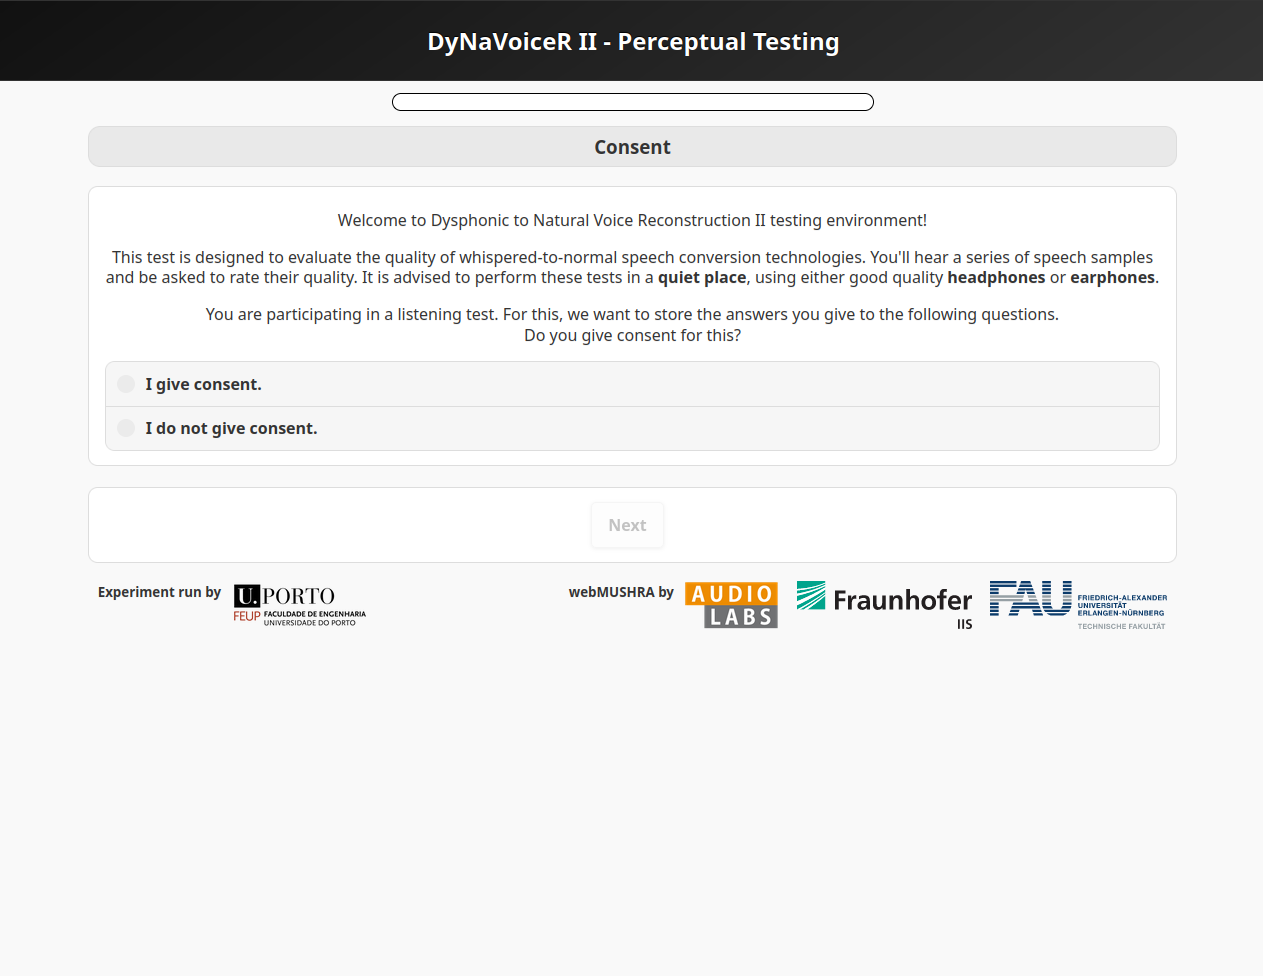
\includegraphics[width=\textwidth]{chapter7/consent.png}
    \caption{Test introduction, contextualization and consent form}
    \label{fig:consent}
\end{figure}

\begin{figure}[H]
    \centering
    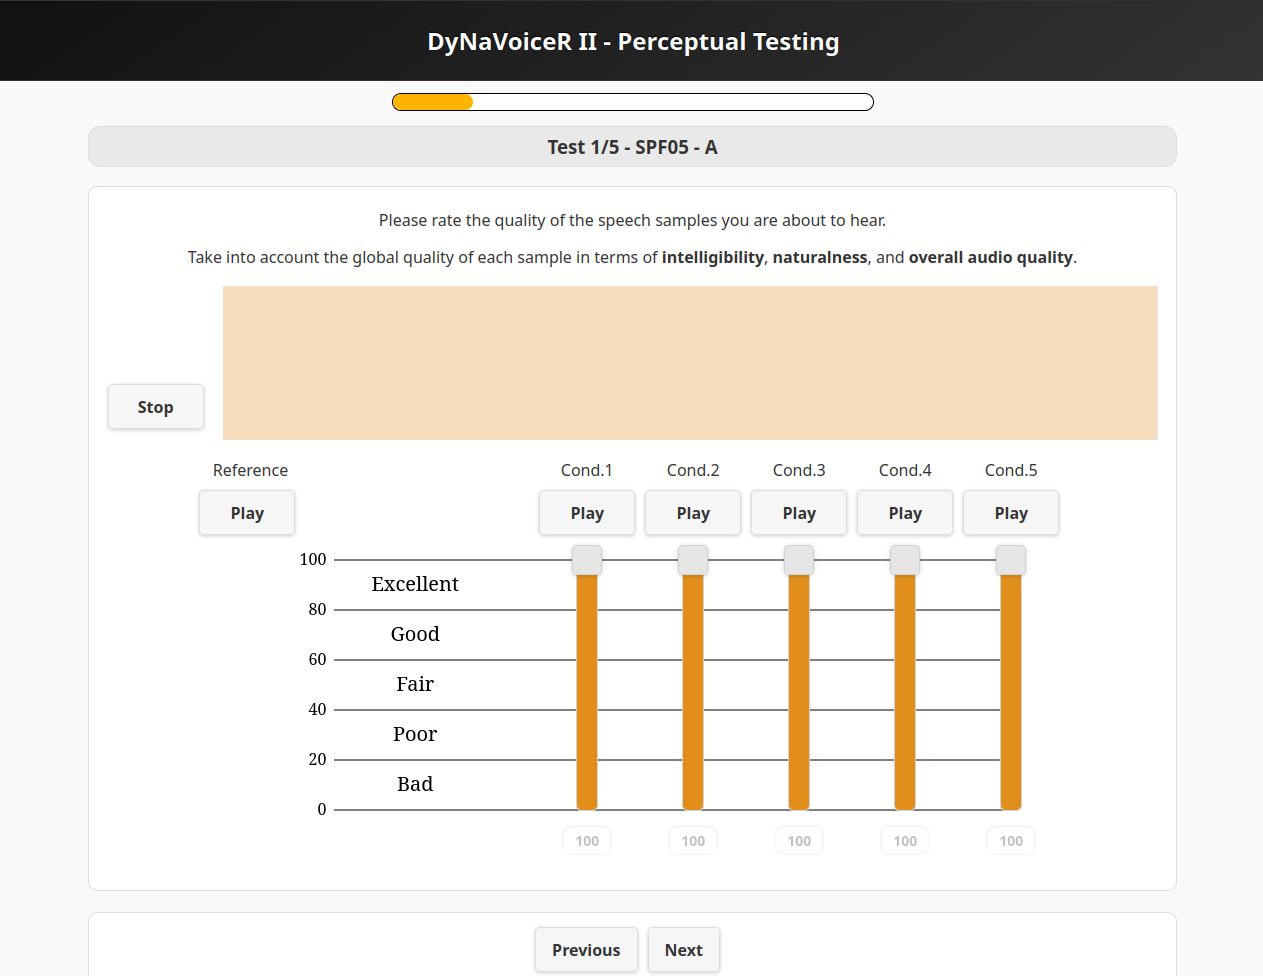
\includegraphics[width=\textwidth]{chapter7/w2s.png}
    \caption{Whispered to Speech test page}
    \label{fig:mushraW2C}
\end{figure}

\begin{figure}[H]
    \centering
    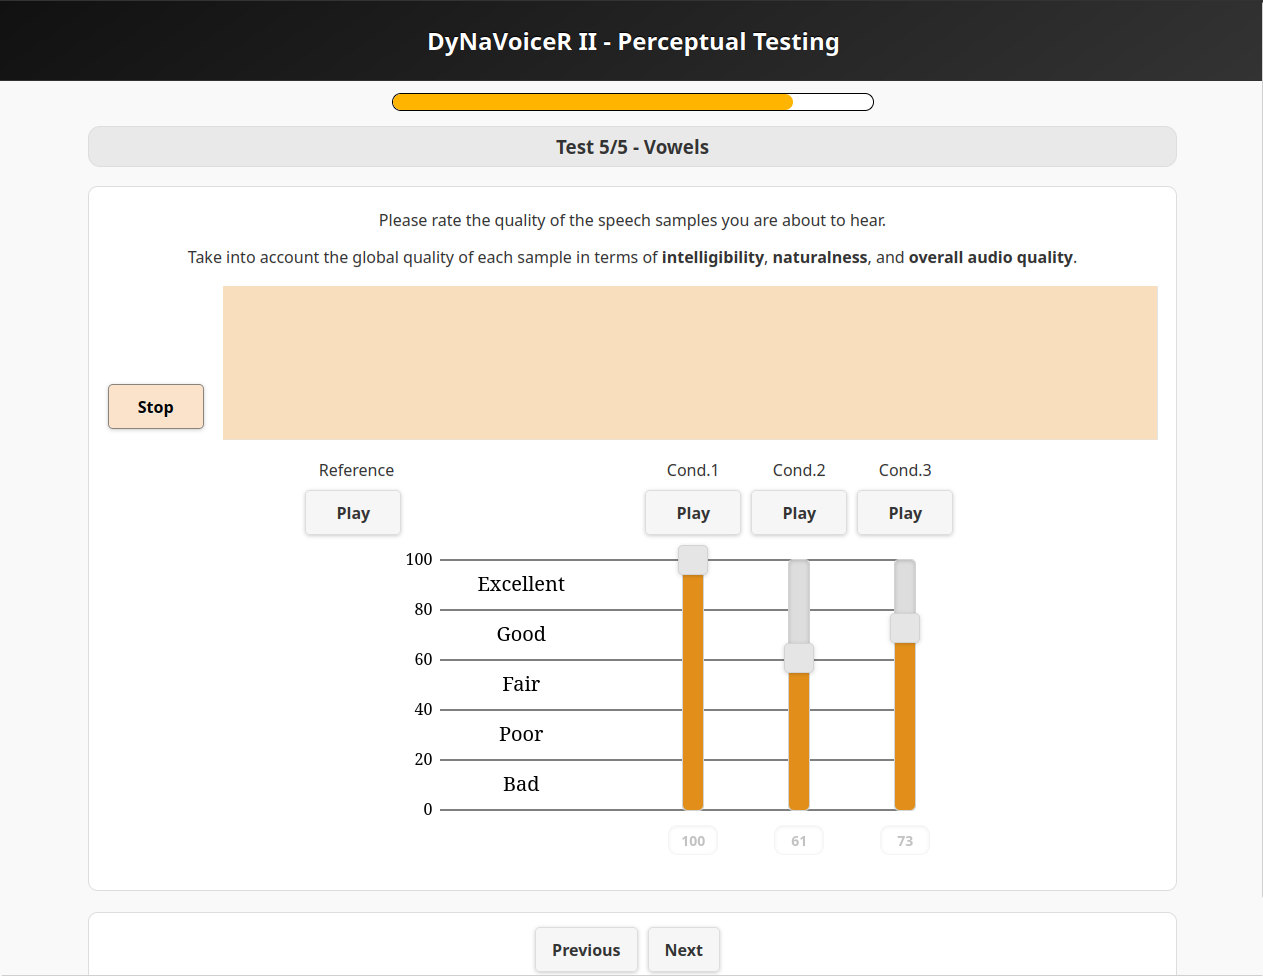
\includegraphics[width=\textwidth]{chapter7/vowel.png}
    \caption{Synthetic vowel test page}
    \label{fig:mushraVowel}
\end{figure}

\begin{figure}[H]
    \centering
    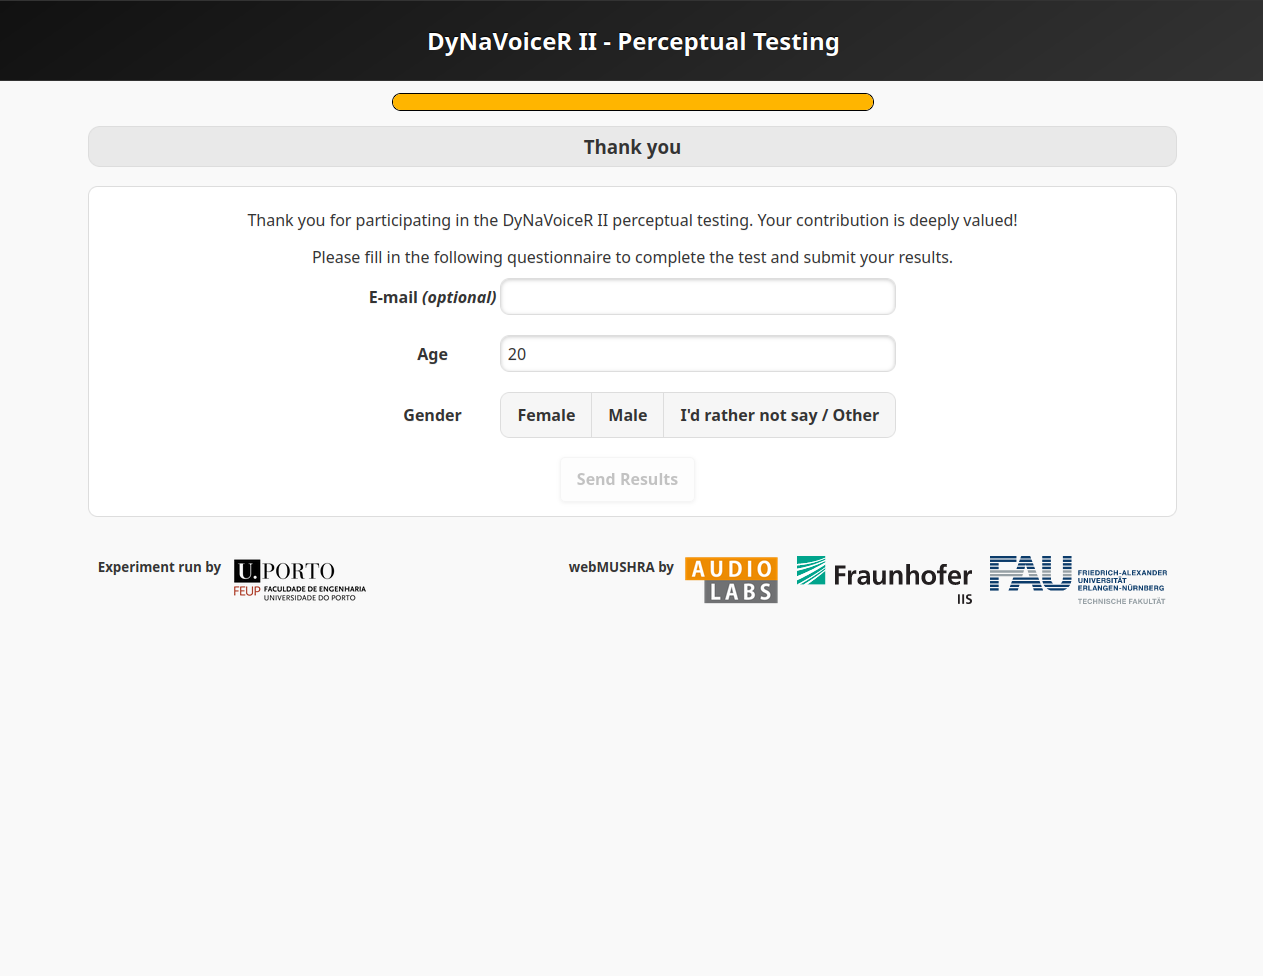
\includegraphics[width=\textwidth]{chapter7/final.png}
    \caption{Final page with feedback form}
    \label{fig:final}
\end{figure}

\section{t-Testing results}

\begin{table}[H]
    \centering
    \begin{tabular}{lccccc}
        \hline
        & Reference & Whispered & FrameFilt & PulseFilt & Segmented \\
        \hline
        Reference & - & 4.46e-02 & 1.77e-12 & 6.83e-13 & 1.34e-09 \\
        Whispered & 4.46e-02 & - & 3.94e-11 & 5.23e-09 & 2.45e-07 \\
        FrameFilt & 1.77e-12 & 3.94e-11 & - & 2.07e-01 & 9.81e-07 \\
        PulseFilt & 6.83e-13 & 5.23e-09 & 2.07e-01 & - & 5.22e-06 \\
        Segmented & 1.34e-09 & 2.45e-07 & 9.81e-07 & 5.22e-06 & - \\
        \hline
    \end{tabular}
    \caption{Pairwise P-Values for subject SPF05}
    \label{tab:pairwiseSPF05}
\end{table}

\begin{table}[H]
    \centering
    \begin{tabular}{lccccc}
        \hline
        & Reference & Whispered & FrameFilt & PulseFilt & Segmented \\
        \hline
        Reference & - & 7.04e-03 & 5.12e-13 & 3.68e-13 & 7.62e-10 \\
        Whispered & 7.04e-03 & - & 1.88e-11 & 1.68e-08 & 2.00e-06 \\
        FrameFilt & 5.12e-13 & 1.88e-11 & - & 1.00e-01 & 4.45e-04 \\
        PulseFilt & 3.68e-13 & 1.68e-08 & 1.00e-01 & - & 1.41e-03 \\
        Segmented & 7.62e-10 & 2.00e-06 & 4.45e-04 & 1.41e-03 & - \\
        \hline
    \end{tabular}
    \caption{Pairwise P-Values for subject SPF12}
    \label{tab:pairwiseSPF12}
\end{table}

\begin{table}[H]
    \centering
    \begin{tabular}{lccccc}
        \hline
        & Reference & Whispered & FrameFilt & PulseFilt & Segmented \\
        \hline
        Reference & - & 1.34e-02 & 2.70e-12 & 5.35e-12 & 1.82e-09 \\
        Whispered & 1.34e-02 & - & 1.05e-09 & 9.62e-09 & 4.17e-07 \\
        FrameFilt & 2.70e-12 & 1.05e-09 & - & 1.49e-01 & 7.39e-05 \\
        PulseFilt & 5.35e-12 & 9.62e-09 & 1.49e-01 & - & 3.95e-04 \\
        Segmented & 1.82e-09 & 4.17e-07 & 7.39e-05 & 3.95e-04 & - \\
        \hline
    \end{tabular}
    \caption{Pairwise P-Values for subject SPM14}
    \label{tab:pairwiseSPM14}
\end{table}

\begin{table}[H]
    \centering
    \begin{tabular}{lccccc}
        \hline
        & Reference & Whispered & FrameFilt & PulseFilt & Segmented \\
        \hline
        Reference & - & 5.70e-02 & 4.95e-11 & 4.71e-11 & 2.55e-08 \\
        Whispered & 5.70e-02 & - & 6.99e-11 & 1.06e-09 & 1.03e-06 \\
        FrameFilt & 4.95e-11 & 6.99e-11 & - & 5.82e-01 & 8.17e-04 \\
        PulseFilt & 4.71e-11 & 1.06e-09 & 5.82e-01 & - & 5.95e-05 \\
        Segmented & 2.55e-08 & 1.03e-06 & 8.17e-04 & 5.95e-05 & - \\
        \hline
    \end{tabular}
    \caption{Pairwise P-Values for subject SPM18}
    \label{tab:pairwiseSPM18}
\end{table}

%%----------------------------------------
%% Final materials
%%----------------------------------------

%% Bibliography
%% Comment the next command if BibTeX file not used
%% bibliography is in ``myrefs.bib''
\PrintBib{myrefs}

%% Index
%% Uncomment next command if index is required
%% don't forget to run ``makeindex thesis'' command
%\PrintIndex

\end{document}
